% !TeX encoding = UTF-8
% !TeX program = pdflatex
% !TeX spellcheck = en_US

\documentclass[binding=0.6cm]{sapthesis}

\usepackage{microtype}
\usepackage[english]{babel}
\usepackage[utf8]{inputenc}
\usepackage{subcaption}
\usepackage{placeins}
\usepackage{hyperref}
%\hypersetup{pdftitle={Lightweight Scene Understanding and Synthetic Data-Driven Damage Inspection for Martian Rovers},pdfauthor={Daniele Venturini}}

\hypersetup{
%			hyperfootnotes=true,			
%			bookmarks=true,			
			colorlinks=true,
			linkcolor=red,
            linktoc=page,
			anchorcolor=black,
			citecolor=red,
			urlcolor=blue,
			pdftitle={Lightweight Scene Understanding and Synthetic Data-Driven Damage Inspection for Martian Rovers},
            pdfauthor={Daniele Venturini},
			pdfkeywords={thesis, sapienza, roma, university}
 }

\title{Lightweight Scene Understanding and Synthetic Data-Driven Damage Inspection for Martian Rovers}
\author{Daniele Venturini}
\IDnumber{1991255}
\course{Master's Degree in Computer Science}
\courseorganizer{Faculty of Information Engineering, Informatics, and Statistics}
\AcademicYear{2025/2026}
\advisor{Prof. Marco Raoul Marini}
%\coadvisor{}
\authoremail{venturini.1991255@studenti.uniroma1.it}
\copyyear{2026}
\thesistype{Master's Degree Thesis}
\examdate{27 October 2026}
\examiner[]{Prof. Galasso}
\examiner[Thesis Advisor]{Prof. Marini}
\examiner[]{Prof. Carlucci}
\examiner[]{Prof. Perelli}
\examiner[]{Prof. Pontarelli}
\examiner[]{Prof. Spinelli}
\examiner[]{Prof. Sterbini}
\versiondate{1.048596}

\begin{document}

\frontmatter
\maketitle
\dedication{"Even if it's over now, \\ I'm glad we stopped to hear the music"}

\begin{acknowledgments}
	Certo! Ecco una versione generica di ringraziamenti da scrivere in una tesi magistrale:
	Purtroppo questa volta devo fare le cose per bene e ciò include fare i ringraziamenti. Per renderli speciali, sarà anche l'unica parte di tesi scritta senza aiuti artificiali coff coff.
	Il che sarà molto difficile dato che non so come si scrivano bene.

	Per iniziare vorrei ringraziare la mia famiglia, così possono leggere la loro parte tenendo nascosta la seconda parte.
	Ringrazio mia sorella, principalmente perché mi ha sopportato con non tanta pazienza durante tutti questi anni. Quando rientri a casa sappiamo che avrai mille cose da raccontare e di cui lamentarti, ma parliamo anche di cose buone dai, sei la spalla perfetta per vedere film e serie tv, soprattutto horror.
	Un grazie a mio padre, il tuttofare, che so mi avresti voluto mandare a lavorare molto prima, ma mi hai sempre supportato in questo lungo percorso, anche quando ho scelto di continuare e fare anche la magistrale. Sei il mio punto di riferimento su cui posso fare affidamento per tutto, ed è anche grazie a te che ho preso questa passione per l'informatica (ed ora sei te a chiedere consigli a me su questo).
	Un grazie anche a te mamma, per avermi permesso di fare questo percorso, per essere sempre disponibile, per prenderti sempre cura di noi, per avermi insegnato a cucinare e fare buonissimi dolci, per avermi sempre incoraggiato a fare quel che mi piaceva. Sei una forza della natura e mi dai sempre la forza di andare avanti.
	Ospite speciale dei ringraziamenti Nina, il piccolo demone a casa, che in questi quasi 3 anni ha continuamente provato a mangiarci le mani o le braccia, ma a me fa le fusa.

	Ora per la seconda parte, mi raccomando leggetevi solo la vostra parte.
	Inizierei ringraziando i colleghi universitari\texttrademark~che mi hanno accompagnato in questi anni di magistrale. Una presenza constante e ineluttabile è stato Federico, iniziando questo percorso insieme e scegliendo i corsi in modo da poterli seguire insieme (chiaramente i peggiori). Ma sappiamo entrambi che l'università era solo la side quest e il tuo obiettivo era solo farmi spendere soldi in vari giochi. Tra poco con uno stipendio sarà più difficile dirti di no. Colgo l'occasione anche per farti gli auguri per la tua futura laurea (domani) e per la sfida del dottorato, i fusi orari non ci fermeranno.
	Cambiamo una lettera e troviamo Federica, compagna di non so quanti progetti di gruppo e poi anche del percorso di eccellenza\textsuperscript{\copyright}. Felice di averli fatti con te perchè so che sei una persona affidabile, e credo pensai lo stesso di me, sei sempre un po' criptica.
	E poi Diana, amica sempre presente nel bene e nel male dai primi giorni di università. Tra ritiri in aula studio, PAUSE CAFFE' (infinite), lezioni, qualche spritzino, scleri contro i professori, non c'era giornata che non ravvivavi.
	Menzione d'onore a quello che io ho sempre chiamato il "Gruppo di Roma", colleghi di innumerevoli serate sobrie e tranquille. Dopo una breve pausa e con qualche new entry, abbiamo avuto la geniale idea di riunirci per riportare caos e imprevedibilità (non sai mai quando ti arriva il messaggio "STASERA SI ESCE").
	Particolare attenzione anche al "Gruppo del DND" o giochi da tavolo o vacanze a case di Federico. Insomma un sacco di roba.  Mi dispiace per i due master che devono gestire 4 bambini che non sanno ragionare, ma tra i meme e scene iconice, anche oltre alla campagna, rendono le sessioni e le scampagnate infinitamente divertenti ed esotiche.

	Infine e per meno importanza, chiaramente, gli Apriliani\texttrademark.
	Federico, quando non è mese di esami, so che posso sempre contare su di te per le idee più strampalate e all'ultimo secondo, e tu sai lo stesso di me. Ciò non toglie anche i vari discorsi filosofici, politici, utopici, in cui ogni volta facciamo finta di essere dei sapientoni e poi arriviamo sempre alla stessa conclusione: [Redacted for legal reasons].
	E poi c'è Tommaso, la spalla di affidamento, "collega di lavoro", il troppo occupato con i lavori, il principale detentore del contratto di mantenimento, l'avventuriero, l'anfora d'oro. Insomma, un sacco di cose. Ne abbiamo passate mooolte insieme, ma sei stato sempre presente, anche nei momenti più difficili, dimostrando la persona che sei e per questo te ne sono molto grato. Mi raccomando che anche te dovrai far parte dei numerosi piani che prepariamo nei discorsi apriliani filosofici.

	Per concludere mi permetto anche un breve spazio egocentrico, perchè sì sono i miei ringraziamenti in fondo. Impossibile negarlo, sono stati due anni difficili, in cui ho quasi perso l'interesse e l'ambizione con cui avevo iniziato questo percorso, per poi ritrovarli e motivarmi ancora più di prima. Questo lo devo alle persone che ho incontrato, anche per brevi periodi, e a chi mi ha accompagnato dall'inizio o anche prima. Ringrazio me stesso per credere sempre in me e per continuare a lottare per raggiungere i miei obiettivi, nonostante tutto.
\end{acknowledgments}

\raggedbottom

\begin{abstract}
	This thesis investigates two applications for Martian rover autonomy: lightweight semantic scene understanding for navigation support and automated inspection of visible wheel damage. Segmentation architectures are evaluated on S5Mars, together with quantization strategies to reduce inference cost. SegFormer-B0 reaches 76.93\% test mean Intersection over Union after Quantization-Aware Training, while DeepLabV3+ with MobileNetV2 requires the least measured GPU energy per image. Separate MarsSeg experiments show better cross-mission transfer for SegFormer-B0 than for the tested convolutional models.

	For damage inspection, no suitable real-image benchmark with perforation masks was identified. An automated Blender pipeline therefore generates 10,000 annotated images of a Curiosity model, including matched normal and perforated wheel observations. Synthetic generation avoids extensive manual labeling while providing automatic ground truth and controlled variation of damage and imaging conditions. Four anomaly detection families are evaluated using only normal renders for training. On the overhead-view test subset, PatchCore Large achieves an image-level area under the receiver operating characteristic curve of 86.43\%, whereas a compact TinyGLASS configuration has the lowest measured inference cost. Detection and localization results show that better image discrimination does not necessarily imply more precise damage maps. The findings provide an experimental basis for terrain interpretation and targeted wheel inspection, adaptation across the synthetic-to-real gap and measurements on representative hardware. Future integration could use the predicted \emph{Rover} region to guide a dedicated wheel localizer before applying the damage detector, combining navigation support and targeted inspection within a common onboard perception pipeline.
\end{abstract}

\tableofcontents

\mainmatter
\chapter{Introduction}

\section{Problem Statement}

Mars rover operations require interpreting the surrounding terrain while preserving the vehicle's ability to move through it. Ground teams can examine images and plan subsequent activities, but communication with Earth does not permit immediate intervention during a drive, because the one-way light time varies from approximately 4 to 22 minutes \cite{nasaJPL2022Driving}. Visual processing performed locally could therefore support decisions about terrain and provide information about the condition of exposed rover components. This thesis investigates two complementary aspects of that problem: lightweight semantic scene understanding and visual inspection of wheel damage.

Semantic segmentation assigns a category to each image pixel, producing a spatial description of the observed scene. For rover navigation, this representation can distinguish materials and features whose relevance is not fully captured by geometry alone. Sand and bedrock, for example, have different implications for traversability, motivating terrain-aware perception rather than obstacle detection based exclusively on shape \cite{swan2021ai4mars}. However, potential onboard use also requires attention to inference cost. A model with accurate predictions may still require excessive computation or memory for the intended platform, which motivates studying segmentation quality together with latency, energy consumption, and memory requirements \cite{xiong2024light4mars}.

Wheel inspection addresses a different visual question. Curiosity has experienced cracks, tears, and perforations in its aluminum wheel skin, as well as broken traction features, and these changes are monitored through periodic imaging \cite{rankin2022wheelassessment}. Figure~\ref{fig:curiosity-wheel-damage} shows a real example of visible wheel damage that motivates this work. Detecting a damaged observation and locating the affected region could support the review of inspection images. The task considered here is restricted to visible wheel perforations, whose appearance must be distinguished from shadows, dust, and surface wear that do not belong to the modeled damage class. By highlighting regions that may require closer inspection, this approach can support the review of wheel images and help track visible damage across successive observations.

\begin{figure}[htbp]
    \centering
    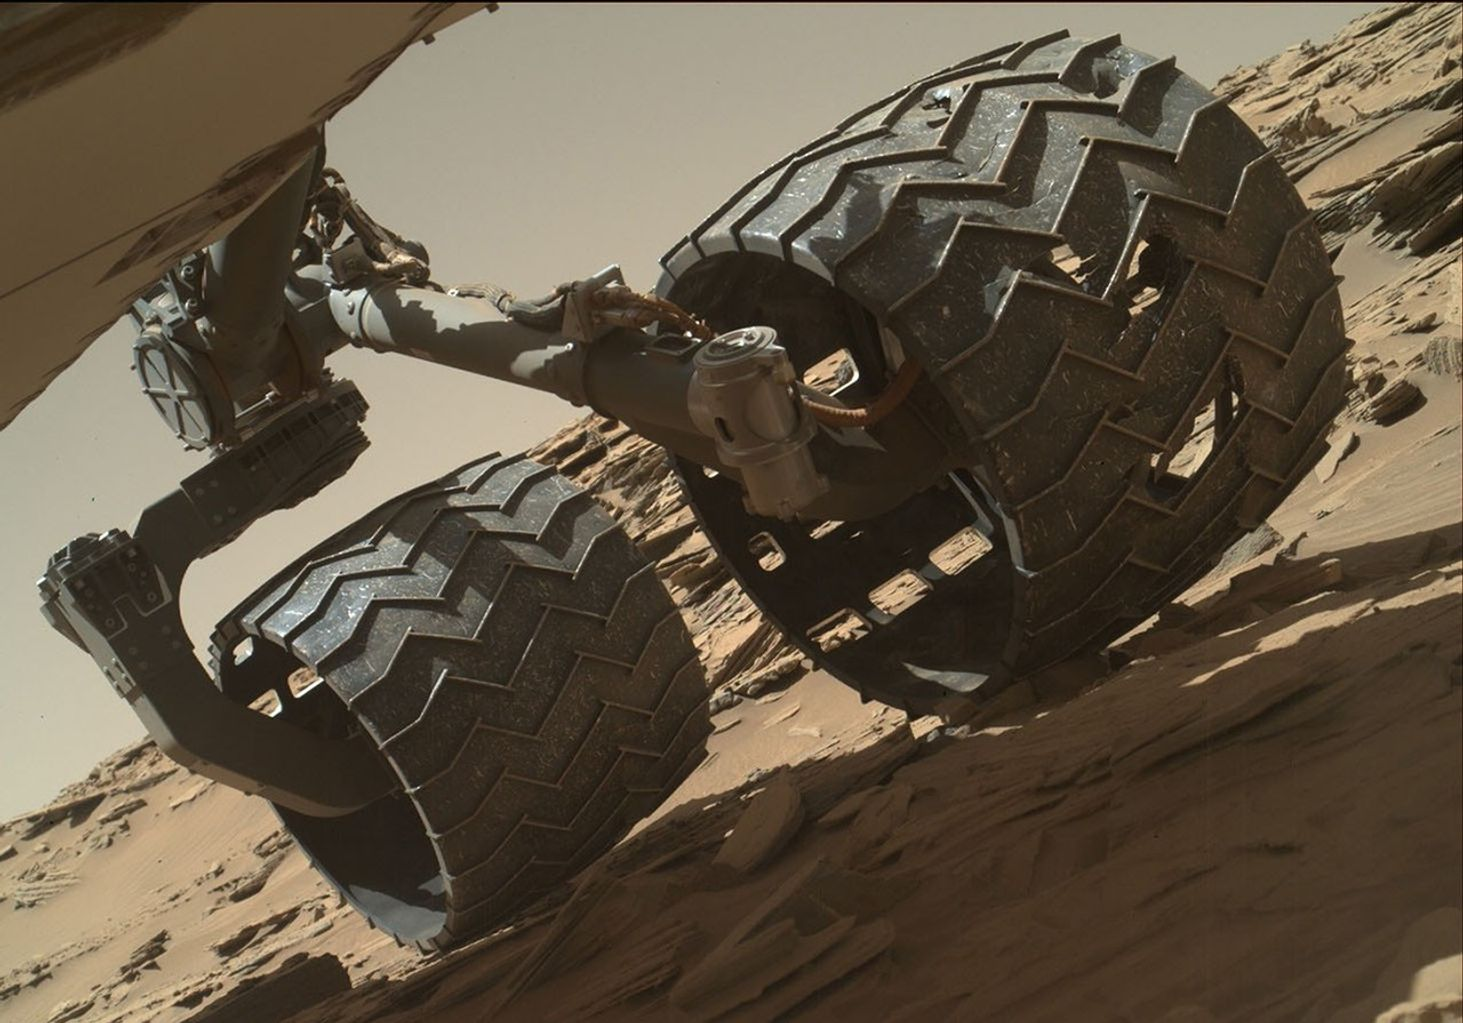
\includegraphics[width=0.85\textwidth]{Images/curiosity_wheel_damage_PIA20334.jpg}
    \caption{Curiosity's left-middle and left-rear wheels imaged by the Mars Hand Lens Imager on sol 1315 (18 April 2016). An irregular tear in the aluminum wheel skin is visible in the upper portion of the wheel on the right \cite{nasa2016wheelinspection}.}
    \label{fig:curiosity-wheel-damage}
\end{figure}

The main constraint in this second branch is the availability of suitable labeled data. Public rover imagery provides relevant observations, but the resources examined for this work did not supply a ready-to-use benchmark with the perforation annotations required for detection and pixel-level localization. A dedicated synthetic dataset was therefore constructed to provide controlled wheel observations and automatically derived damage masks. The inspection models are trained on normal images, reducing their dependence on annotated damage examples during training, while normal and damaged observations are used for evaluation.

The shared objective is to establish which visual methods provide useful information at an acceptable computational cost under these two experimental settings. Scene understanding is evaluated on real rover images, whereas the main damage inspection experiments use generated images of a Curiosity asset. The two branches contribute to the same long term goal of rover autonomy, while using separate datasets, methods, and evaluations.

\section{State of the Art}

The relevant literature concerns both the interpretation of Martian environments and the inspection of localized defects. Dataset design is central to both problems, because the available annotations determine which visual questions can be studied. The following review first considers rover-scene segmentation, places related work on atmospheric imagery within the broader use of artificial intelligence on Mars, and then examines wheel inspection and synthetic-data-based anomaly detection.

\subsection{Datasets}
AI4Mars, introduced by Swan et al., is a large-scale resource for Martian terrain segmentation. Its authors report approximately 35,000 rover images and 326,000 full-image annotations, with multiple crowdsourced annotations collected for each image and approximately 1,500 expert-produced labels \cite{swan2021ai4mars}. Its semantic scope, however, is limited to four terrain categories: \emph{Soil}, \emph{Bedrock}, \emph{Sand}, and \emph{Big Rock}. Pixels overlapping the rover are removed from the terrain annotations through auxiliary masks rather than being represented by a trainable \emph{Rover} category \cite{swan2021ai4mars}. AI4Mars therefore provides neither the range of environmental categories available in the selected S\textsuperscript{5}Mars release nor the rover-level semantic information relevant to the broader aims of this thesis.

Annotation quality was another reason to choose a different primary benchmark. The Mars-Bench authors identified errors in AI4Mars annotations during an expert review and excluded the dataset from their benchmark \cite{purohit2025marsbench}. AI4Mars did include quality checks, multiple annotations per image, and an expert-labeled validation subset \cite{swan2021ai4mars}. However, the concerns raised by the Mars-Bench review, together with the limited set of terrain categories and the lack of a semantic \emph{Rover} category, motivated the choice of another dataset for this work.

S\textsuperscript{5}Mars takes a different approach to the shortage of labeled data. Zhang et al. introduce 6,000 high-resolution Curiosity images, labeling only regions that can be interpreted with confidence. Their semi-supervised method combines image augmentations suited to Martian scenes with consistency learning that considers how confident the model is in its predictions \cite{zhang2024s5mars}. This approach allows training with incomplete annotations while accounting for uncertainty in both the labels and the model predictions.

Mars-Bench subsequently provides standardized dataset formats and predefined splits for several Martian vision tasks. Its S\textsuperscript{5}Mars adaptation merges visually ambiguous granular material categories into \emph{Sand/Soil} following expert review, while keeping environmental categories and a \emph{Rover} category \cite{purohit2025marsbench}. This release is adopted here to support reproducible segmentation experiments. Its rover label also provides a possible future interface with inspection, although identifying rover pixels alone does not identify individual wheels or their defects.

\subsection{Semantic Segmentation and Efficient Rover Perception}

Mars specific segmentation research has examined how to preserve local detail while incorporating the context needed to distinguish similar surface materials. Li et al. propose MarsSeg, an encoder--decoder network that enhances and combines features at multiple levels, with attention mechanisms directed toward semantic information and spatial detail \cite{li2025marsseg}. The method illustrates the relevance of both scales: small terrain elements require fine image information, whereas their interpretation can depend on the surrounding scene. These observations motivate comparing architectures with different approaches to context extraction and reconstruction.

Computational efficiency introduces an additional design criterion. Light4Mars, proposed by Xiong et al., targets semantic segmentation in unstructured Martian environments using a lightweight Transformer architecture. Its experimental resources include the synthetic SynMars-TW dataset and real Curiosity imagery in MarsScapes \cite{xiong2024light4mars}.

General segmentation architectures offer complementary reference points. U-Net combines a contracting path with an expanding path for localization, DeepLab uses atrous convolutions to incorporate context, and SegFormer combines hierarchical Transformer features with a compact decoding head \cite{ronneberger2015unet,chen2017deeplabv3,xie2021segformer}. The present study uses these established families alongside lightweight alternatives to investigate the accuracy-efficiency trade-off on a common rover-image task. It also examines reduced-precision execution, because architecture selection and deployment configuration both affect the resources required for inference.

The application of segmentation to Mars extends beyond rover-acquired surface images. For example, Barrett et al. use semantic segmentation of orbital images to produce terrain maps for the ExoMars candidate landing sites at Oxia Planum and Mawrth Vallis \cite{barrett2022noahh}. In \cite{venturini2025duststorms} the authors study dust storm segmentation in global maps derived from orbital observations. Their approach enhances U-Net with channel and spatial attention and addresses class imbalance and missing-data artifacts in the maps.

% This work is relevant as a related application of artificial intelligence to Martian imagery, where the learning procedure must account for the characteristics of the observations and the target phenomenon. Its attention-based feature refinement and consideration of model size connect with the broader interest in useful segmentation at manageable computational cost. The atmospheric task nevertheless differs from rover terrain segmentation in acquisition geometry, target labels, and data preparation. It therefore informs the research context without serving as an onboard rover model or a baseline for the experiments in this thesis.

\subsection{Wheel Damage Inspection and Available Imagery}

Wheel perforations are a documented form of damage experienced by NASA's Curiosity rover. Official images acquired by the Mars Hand Lens Imager (MAHLI) show holes and tears in the aluminum wheel skin, which have been monitored through periodic wheel inspections \cite{nasa2016wheelinspection}. In the ground-based procedure described by Rankin et al., the Wheel Wear team examines downlinked images, compares them with previous observations, and manually measures damage features to track their progression \cite{rankin2022wheelassessment}. This operational context motivates investigating automated visual inspection as a means of supporting damage detection and localization.

The availability of wheel images does not, however, imply the availability of annotations suited to that task. The public Curiosity image classification dataset released by Lu and Wagstaff includes a generic wheel category, but provides image-level content labels rather than annotations of individual perforations or pixel-level damage masks \cite{lu2020mslimages}. A model trained to recognize an image as containing a wheel would therefore answer a different question from whether that wheel contains a visible hole.

Among the public resources examined for this work, no ready-to-use benchmark was identified that combined perforation-specific annotations with the experimental task required by the damage-inspection study. A dedicated dataset was needed, and synthetic generation was selected instead of manually curating and densely annotating a real-image corpus within the time available. This choice also enabled controlled variation of the damage and imaging conditions, with annotations derived directly from the generated scenes. The resulting dataset supports an experimental study of visible perforations, while broader wheel failure modes remain outside its scope.

\subsection{Visual Anomaly Detection and Synthetic Data}

Industrial visual anomaly detection provides a relevant methodological setting when annotated defects are scarce. The MVTec Anomaly Detection (MVTec AD) dataset uses defect-free images for training and includes normal and defective test images with spatial annotations, allowing detection and localization to be evaluated separately \cite{bergmann2019mvtec}. The same distinction is useful for wheel inspection, because ranking a damaged image above a normal one does not establish that the defect has been precisely delineated.

Different anomaly-detection families represent normal appearance in different ways. PatchCore stores representative features from normal image patches in a memory bank \cite{roth2022patchcore}, whereas EfficientAD trains a compact student network to reproduce features extracted from normal images by a teacher \cite{batzner2024efficientad}. SuperSimpleNet supports both normal-only and supervised training settings \cite{rolih2025supersimplenet}. TinyGLASS further investigates compact anomaly detection for resource-constrained edge and in-sensor processing \cite{bonazzi2026tinyglass}. These methods motivate comparing damage discrimination and spatial localization together with inference requirements. Their performance on industrial benchmarks does not establish their effectiveness on rover wheels, which must be assessed under the inspection conditions considered here.

Synthetic data provides control over those conditions and a way to obtain spatial annotations without labeling each generated image manually. Tobin et al. investigate domain randomization by varying rendered appearance during training, demonstrating transfer for a robotic object-localization task \cite{tobin2017domain}. This supplies a rationale for introducing visual variation, while transfer to a different application remains an empirical question. In this thesis, rendering is used to construct matched normal and damaged wheel observations under controlled changes in viewpoint, illumination, and surface appearance. These controlled comparisons provide a foundation for adapting and evaluating inspection methods on real rover images, with the longer-term aim of supporting automated wheel monitoring during rover operations.

\section{Proposed Research Framework}

The research framework contains two experimental branches linked by the objective of providing visual information for rover autonomy. The scene-understanding branch studies semantic labels for the surrounding environment, while the inspection branch studies evidence of visible wheel perforations. Each branch uses its own dataset and evaluation procedure to address its specific challenges.

For scene understanding, the Mars-Bench release of S\textsuperscript{5}Mars provides the primary task. Seven segmentation configurations are compared across U-Net, DeepLabV3, DeepLabV3+, SegFormer-B0, and two LCNet variants, using different convolutional backbones where possible. The study examines segmentation quality and resource requirements, then evaluates reduced-precision deployments through a comparison between Post-Training Quantization and Quantization-Aware Training. A separate experiment uses the taxonomy compatible MarsSeg datasets to examine transfer between Curiosity imagery and images from Spirit and Opportunity without fine-tuning. This extends the analysis beyond performance on a single acquisition domain and helps study the generalization of the proposed models.

For wheel inspection, an automated Blender pipeline generates observations of the six wheels of a Curiosity model. Camera viewpoint, wheel rotation, lighting, and benign surface wear are varied, while localized through-holes define the anomaly class. Normal and damaged counterparts share the same acquisition and appearance parameters so that the introduced perforation is the intended difference within each pair. Target-wheel masks and damage masks are derived from the scenes, and paired observations remain within the same split to prevent leakage between partitions.

PatchCore, EfficientAD-S, SuperSimpleNet, and TinyGLASS are then adapted and evaluated using normal-only training data. The principal comparison uses a controlled camera viewpoint and wheel-focused inputs, while additional experiments examine selected acquisition and model settings. Image-level scores assess damage discrimination, and spatial maps assess localization. Validation data informs configuration selection and calibration, with the test split providing a separate assessment of the retained configurations. Latency, GPU energy, and memory measurements complement the accuracy metrics in both branches.

% The framework addresses three objectives:
% \begin{enumerate}
%     \item Determine how the tested segmentation architectures and deployment configurations balance semantic accuracy with inference resource requirements on Martian rover imagery.
%     \item Construct a synthetic dataset that permits controlled evaluation of visible wheel perforations, with spatial annotations and matched normal/damaged observations.
%     \item Assess how established normal only anomaly detection methods balance image-level damage discrimination, pixel-level localization, and inference cost in that synthetic setting.
% \end{enumerate}

The framework is evaluated as a set of complementary studies, but the semantic \emph{Rover} category is a possible starting point for future automatic region selection, even though connecting it to wheel localization and damage detection requires additional implementation and evaluation. Likewise, the measured inference costs concern the experimental hardware and do not establish equivalent behavior on rover flight computers.

\section{Main Contributions}

The contributions concern dataset construction, adaptation of established methods, and empirical evaluation. They provide a basis for selecting visual processing configurations that balance prediction quality and computational cost, supporting future integration of scene understanding and wheel inspection into rover perception systems.

\begin{itemize}
    \item \textbf{A comparative study of Martian scene understanding.} Seven segmentation configurations are evaluated on the selected S\textsuperscript{5}Mars release, with analyses of per-class behavior and training choices. Separate MarsSeg experiments examine cross-mission generalization under a shared taxonomy.
    \item \textbf{An assessment of segmentation deployment trade-offs.} Floating-point and quantized configurations are compared using segmentation accuracy, latency, GPU energy per image, and peak GPU memory, examining how reduced precision changes the practical cost of inference.
    \item \textbf{An automated synthetic wheel-damage dataset.} A Blender generation pipeline produces 10,000 annotated images of a Curiosity asset, including 7,000 normal training images. The dataset covers six target-wheel positions and provides target-wheel masks, perforation masks, and matched normal/damaged evaluation pairs, with controlled sampling and quality checks.
    \item \textbf{An evaluation of synthetic-data-driven damage inspection.} Four established anomaly-detection families are adapted to normal-only wheel inspection. The experiments distinguish damage detection from localization and examine selected model settings together with their measured inference requirements.
\end{itemize}

\section{Thesis Organization}

The next three chapters describe the methods. Chapter 2  introduces the semantic-segmentation task, datasets, architectures, training procedure, and deployment optimizations. Chapter 3 presents the Curiosity asset preparation, scene construction, damage generation, annotations, and dataset quality controls. Chapter 4 defines the normal-only inspection setting and describes preprocessing, anomaly-detection methods, and evaluation metrics.

Chapters 5 and 6 present the experimental evidence. Chapter 5 reports segmentation accuracy, quantization results, training ablations, and cross-mission generalization. Chapter 6 compares damage detection, localization, and inference cost, followed by model-specific ablations. Chapter 7 interprets the findings and examines their practical limits, including the gap between generated and real wheel imagery. Chapter 8 summarizes the contributions and identifies further work on real-image validation, broader damage coverage, and eventual system integration.

\chapter{Lightweight Scene Understanding}

\section{Task Definition}
%The first part of the proposed framework deals with obtaining accurate semantic labeling from images captured by the navigation camera on Mars Rover. This is an essential step to aid the rover in achieving autonomous navigation, considering the delay in communications between Mars and Earth and real-time ground control is not practicable.
%In this section a deep-learning approach was implemented to tackle this task, given the vast progress made in semantic segmentation techniques in the field. The main objective was to test several Deep Learning architectures on a novel benchmark dataset [Mars Bench with S5Mars] that provided accurate labels for both terrain segmentation but that could also be useful for the second part in identifying rover parts in the image. Importance was also given to the efficiency of techniques used, looking for a possible on-board deployment that requires a lot of constraint to be effectively operatable, such as ...
%so accuracy-efficiency tradeoff was an important factor used when choosing and optmizing the architectures.

The one-way light time between Earth and Mars varies from approximately 4 to 22 minutes, making continuous remote operations impracticable \cite{nasaJPL2022Driving}. Decisions that must be taken while a rover traverses terrain not yet examined by ground operators therefore benefit from onboard perception and autonomous reasoning. The first branch of the proposed framework addresses this perception problem through semantic segmentation of rover-acquired color images with red, green, and blue channels. More specifically, the experiments presented in this thesis use images captured by the Mast Camera (Mastcam) aboard the Curiosity rover, as provided by the Mars-Bench release of S5Mars \cite{zhang2024s5mars,purohit2025marsbench}. The objective is to convert each observation into a pixel-level representation of the surrounding scene that may support downstream functions such as terrain interpretation, traversability assessment, and route planning.
The dataset was selected because its label space covers terrain elements relevant to environmental understanding while also including a \emph{Rover} category, establishing a possible future interface with the damage-inspection branch.

A deep learning approach is adopted to compare architectures with different representational capacities and computational requirements. The objective is not to maximize segmentation accuracy in isolation, because potential onboard use makes computational efficiency a central design criterion, as also emphasized by previous research on lightweight semantic segmentation for Martian environments \cite{xiong2024light4mars}. The experimental study therefore considers the accuracy-efficiency trade-off and subsequently investigates quantization as a means of reducing inference cost without introducing an unacceptable degradation in segmentation quality.

\section{Dataset}
The primary dataset adopted for the scene-understanding experiments is the Mars-Bench adaptation of S\textsuperscript{5}Mars. The original S\textsuperscript{5}Mars dataset was introduced by Zhang et al. for semi-supervised semantic segmentation of Martian scenes \cite{zhang2024s5mars}. It comprises 6,000 RGB images acquired by Mastcam aboard the Curiosity rover, each with a spatial resolution of 1200 \(\times\) 1200 pixels. Its annotations follow a sparse, confidence-based annotation procedure, where instead of assigning a category to every pixel, labels are retained only in regions for which the annotators considered the semantic interpretation sufficiently reliable. This design limits uncertain assignments at visually ambiguous boundaries, but also leaves part of each mask without a terrain label.

The Mars-Bench release was selected in preference to the original distribution to obtain a more reproducible and internally consistent evaluation setup. Mars-Bench converts previously published Martian vision datasets into standardized formats and supplies predefined training, validation, and test partitions \cite{purohit2025marsbench}. More importantly, its authors subjected the terrain-segmentation datasets to an additional expert review. They reported ambiguities among visually similar granular-material categories and consolidated the corresponding S\textsuperscript{5}Mars labels into a single \emph{Sand/Soil} category. This refinement was intended to reduce label noise and make comparisons between models less dependent on uncertain distinctions. This Mars-Bench release used in this work contains 4,997 training images, 200 validation images, and 800 test images. Mars-Bench describes eight target categories, while the released masks expose an additional \emph{Background} identifier, even though no ground truth mask includes this class. Nonetheless, the implementation uses nine mask identifiers: \emph{Background}, \emph{Bedrock}, \emph{Hole}, \emph{Ridge}, \emph{Rock}, \emph{Rover}, \emph{Sand/Soil}, \emph{Sky}, and \emph{Track}

Two additional datasets included in Mars-Bench were used for a separate cross-dataset evaluation: MarsSeg MSL and MarsSeg MER \cite{purohit2025marsbench}. Both originate from the MarsSeg dataset family introduced by Li et al. \cite{li2022covda} and were subsequently adapted to the standardized taxonomy and evaluation setup defined by Mars-Bench. MarsSeg MSL comprises RGB Mastcam images acquired by the Curiosity rover during the Mars Science Laboratory (MSL) mission, whereas MarsSeg MER contains grayscale images captured by the Navigation Cameras (Navcams) and Panoramic Cameras (Pancams) aboard the Spirit and Opportunity rovers during the Mars Exploration Rover (MER) missions \cite{li2022covda}. Their identical label mapping permits direct cross-mission evaluation without modifying the output layer or introducing an uncertain correspondence between categories. A model can be trained and selected using one mission and subsequently evaluated, without target-domain fine-tuning, on the test split of the other.

\begin{table}[ht]
    \centering
    \resizebox{\linewidth}{!}{%
        \begin{tabular}{@{}l l c r r r@{}}
            \toprule
            \textbf{Dataset}              &
            \textbf{Rover(s) / Sensor(s)} &
            \textbf{Mask IDs}             &
            \textbf{Training}             &
            \textbf{Validation}           &
            \textbf{Test}                                                                            \\
            \midrule
            \midrule
            S\textsuperscript{5}Mars
                                          & Curiosity / Mastcam
                                          & 9                                    & 4,997 & 200 & 800 \\
            MarsSeg MSL
                                          & Curiosity / Mastcam
                                          & 7                                    & 2,893 & 413 & 828 \\
            MarsSeg MER
                                          & Spirit, Opportunity / Navcam, Pancam
                                          & 7                                    & 744   & 106 & 214 \\
            \bottomrule
        \end{tabular}%
    }
    \vspace{5mm}
    \caption{Mars-Bench semantic segmentation datasets used in this work.}
    \label{tab:mars-bench-datasets}
\end{table}

\section{Preprocessing}

A consistent input representation was enforced across all dataset splits. Each image was converted to RGB, ensuring a three-channel input irrespective of its original encoding, while the corresponding segmentation mask was retained as a single-channel categorical map. Image-mask pairs were subsequently resized to \(512 \times 512\) pixels, a resolution selected to retain sufficient spatial detail for semantic segmentation. Bilinear interpolation was used for the RGB images, as it provides smooth resampling of continuous intensity values, while nearest-neighbor interpolation was applied to the segmentation masks to prevent the introduction of intermediate values that would not correspond to valid semantic categories.

Data augmentation was implemented as an optional training-only stage after resizing. The available transformations comprised horizontal flipping, vertical flipping and random \(90^{\circ}\) rotations with probability \(0.5\). When the rotation operation was triggered, the number of \(90^{\circ}\) rotations was sampled uniformly from \(k \in \{0,1,2,3\}\). The default configuration disabled augmentation, whereas the augmented configurations activated these transformations explicitly for comparative experiments. Following the optional augmentation stage, images were scaled to the \([0,1]\) range and then channel-wise normalization was performed using the ImageNet mean values and standard deviations. This convention maintains compatibility with the ImageNet-pretrained encoders employed by several of the evaluated architectures. Segmentation masks were instead converted to integer tensors without normalization, thereby preserving their original class identifiers.
No stochastic transformation was applied to the validation or test splits, as their samples underwent only the deterministic operations of RGB conversion, resizing, tensor conversion, and normalization, ensuring that the reported evaluation results were not affected by random data transformations.

\section{Segmentation Architectures}
\label{sec:segmentation-architectures}

The architecture set was selected with two complementary objectives: preserving continuity with the segmentation models considered in Mars-Bench and investigating a sufficiently broad accuracy-efficiency spectrum for potential onboard deployment. Mars-Bench includes U-Net, DeepLabV3+, SegFormer, and DPT among its semantic segmentation baselines \cite{purohit2025marsbench}. Three of these, U-Net, DeepLabV3+, and SegFormer, were retained in this work. DeepLabV3 was added to examine an atrous-convolution architecture without the low-level feature decoder introduced in DeepLabV3+, whereas LCNet\(_{3,7}\) and LCNet\(_{3,11}\) were included as additional lightweight alternatives.

The resulting model pool comprises seven configurations and covers four substantially different design principles: skip-connected convolutional encoder-decoders, atrous spatial pyramid pooling, hierarchical Transformer representations, and partial-channel transformations. This diversity makes it possible to investigate whether the gains associated with increasingly expressive context modeling justify their computational cost. % At the same time, the experiments presented in this thesis should not be interpreted as a strict reproduction of the Mars-Bench baseline study. The selected backbones, initialization schemes, optimization procedure, and evaluation protocol are specific to the present work; the relationship with Mars-Bench is therefore one of architectural continuity rather than direct leaderboard comparability.

For the S5Mars experiments, every architecture received a three-channel image resized to \(512 \times 512\) pixels and produced nine channels of class scores at the same spatial resolution, one for each class in the taxonomy. The U-Net, DeepLab, and SegFormer configurations returned logits without a final activation, whereas the project LCNet classifiers applied batch normalization and SELU after the final pointwise convolution. The training objective operated on these scores without an additional output softmax. All network components were left trainable.

The U-Net and DeepLab configurations were instantiated through the Segmentation Models PyTorch library \cite{iakubovskii2019smp}. Their encoders were initialized using weights learned on ImageNet, while their decoders and segmentation heads were initialized for the target task. SegFormer-B0 was instead initialized from a checkpoint fine-tuned for semantic segmentation on ADE20K \cite{nvidiaSegformerB0}, with its incompatible 150-class classifier replaced by a nine-channel layer, while the compatible encoder and decoding weights were retained. The two LCNet configurations were trained from random initialization, given the absence of pretrained weights. Consequently, comparisons among different model families capture the behavior of complete deployment candidates, including their initialization strategy, and should not be interpreted as controlled ablations of architecture alone.

\subsection{U-Net Variants}

% U-Net is a Convolutional Neural Network (CNN) Architecture, that follows a symmetric encoder-decoder organization originally introduced for biomedical image segmentation \cite{ronneberger2015unet}. Its contracting path progressively reduces the spatial resolution of the input while extracting increasingly abstract representations, allowing the network to incorporate a broader image context. The expanding path reverses this process and reconstructs a dense prediction at progressively finer resolutions. The defining feature of the architecture is the set of skip connections between corresponding encoder and decoder stages. These connections transfer higher-resolution features directly to the decoding path, where they are combined with more contextual but spatially coarser representations. The decoder can therefore recover local information that would otherwise be weakened by repeated downsampling. This property makes U-Net a suitable conventional and efficient baseline for terrain segmentation, where the accurate localization of class boundaries is important.

U-Net is a convolutional neural network (CNN) with an encoder-decoder architecture originally proposed for biomedical image segmentation \cite{ronneberger2015unet}. The contracting path reduces the spatial resolution of the input and extracts increasingly abstract representations, enabling the network to encode a wider image context. The expanding path restores a dense output at progressively higher resolutions. The defining characteristic of this architecture is the set of skip connections between corresponding encoder and decoder stages. These connections pass higher-resolution features directly to the decoder, where they can be combined with features that contain more context but less spatial detail. The decoder can therefore recover local information that may be weakened by repeated downsampling. This makes U-Net an appropriate baseline for terrain segmentation, where accurate class-boundary localization is important.

\begin{figure}[ht!]
    \centering
    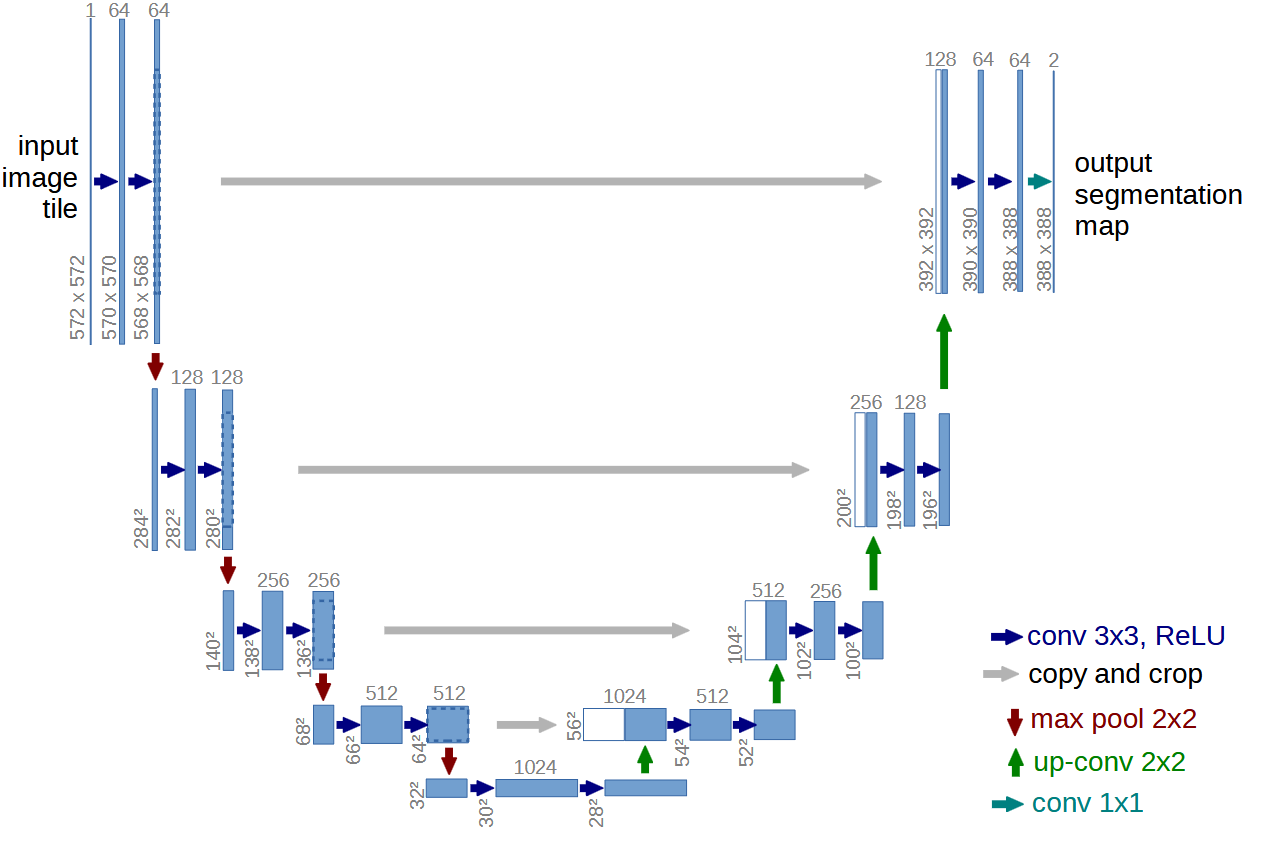
\includegraphics[width=0.95\textwidth]{Images/original-unet.png}
    \vspace{3mm}
    \caption{The original U-Net architecture proposed by Ronneberger et al., comprising a contracting path, an expanding path, and skip connections between corresponding resolution levels \cite{ronneberger2015unet}. The implementations evaluated in this work replace the original contracting path with ResNet34 or MobileNetV2.}
    \label{fig:unet}
\end{figure}

% Both U-Net configurations employed a five-stage decoder, where at each stage the decoder representation was upsampled using nearest-neighbor interpolation, concatenated with the corresponding encoder feature map, and processed by two convolutional blocks with batch normalization and ReLU activation.
Both U-Net variants had a five-stage decoder where, at each stage, the decoder representation was upscaled using nearest-neighbor interpolation and concatenated with the corresponding encoder representation followed by two \(3 \times 3\) convolutional blocks with batch normalization and ReLU activation. A final \(3 \times 3\) segmentation head mapped the resulting 16-channel representation to the nine output classes.

\paragraph{U-Net with ResNet34.}

The first variant makes use of ResNet34 as the encoder. ResNets are a type of architecture that stacks the convolutional layers in blocks where the learned transformation of the block is added to the original block input via a shortcut connection \cite{he2016resnet}. Therefore, every block learns to correct the original representation rather than learning a completely new transformation. ResNet was proposed by He et al. as a way of solving the optimization degradation problem that is experienced when increasing the depth of the conventional convolutional networks. When the input and output dimensions agree, the identity shortcut introduces neither additional parameters nor a separate learned transformation.

In the case of U-Net, ResNet34 provides a conventional hierarchical encoder whose intermediate representations can be transferred to the decoder at different spatial scales. The choice of this architecture was motivated by the fact that it was a higher-capacity convolutional variation in the U-Net family. It combines the established residual feature extractor with an explicit reconstruction path for dense prediction, while preserving architectural continuity with the U-Net baseline considered in Mars-Bench.

The same ResNet34 encoder is also employed in the DeepLabV3 configuration described later in this section. Although the resulting networks are not identical outside the encoder, this shared component makes the comparison between skip-based reconstruction and atrous spatial pyramid pooling (ASPP) easier to interpret.

\paragraph{U-Net with MobileNetV2.}

The second variant replaces ResNet34 with MobileNetV2, an architecture developed specifically for mobile and resource-constrained computer vision \cite{sandler2018mobilenetv2}. MobileNetV2 is an improved version of MobileNetV1, with the aim of optimizing accuracy while ensuring efficiency \cite{lightweight-survey}. Its central component is the inverted residual block.  Whereas the traditional residual block transforms the input representation in the middle of relatively wider representations, MobileNetV2 does this task in between narrower representations, known as bottlenecks. Each block first expands the input representation, performs spatial filtering through an inexpensive depthwise convolution, and then projects the result back to a lower-dimensional space. The final projection is linear, since Sandler et al. observed that applying a non-linearity within a narrow bottleneck can lose useful representational information.

Inside each inverted residual block, depthwise convolution applies a spatial filter independently to every expanded feature channel, whereas the preceding and subsequent pointwise convolutions expand, combine, and project the channel representations. By using spatial filtering and channel mixing in this manner, MobileNetV2 reduces the computational cost associated with typical dense convolutions, while residual connections preserve information between bottleneck representations whenever their spatial resolution and channel dimensionality remain unchanged \cite{sandler2018mobilenetv2}.

The variant was therefore included to determine whether the U-Net topology could provide an effective segmentation model with a substantially lighter encoder. Its comparison with the ResNet34 variant examines two deployment alternatives using the same architectural family: one centered on a conventional residual hierarchy and the other on mobile-oriented inverted residual blocks.

\begin{figure}[ht!]
    \centering
    \begin{subfigure}[t]{0.38\textwidth}
        \centering
        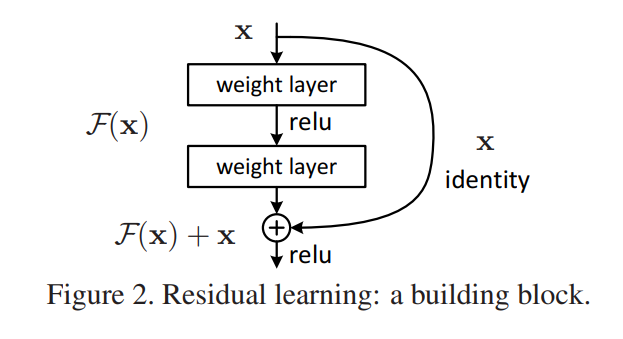
\includegraphics[width=\linewidth]{Images/Residual Connection.png}
        \caption{Residual learning block.}
    \end{subfigure}
    \hfill
    \begin{subfigure}[t]{0.56\textwidth}
        \centering
        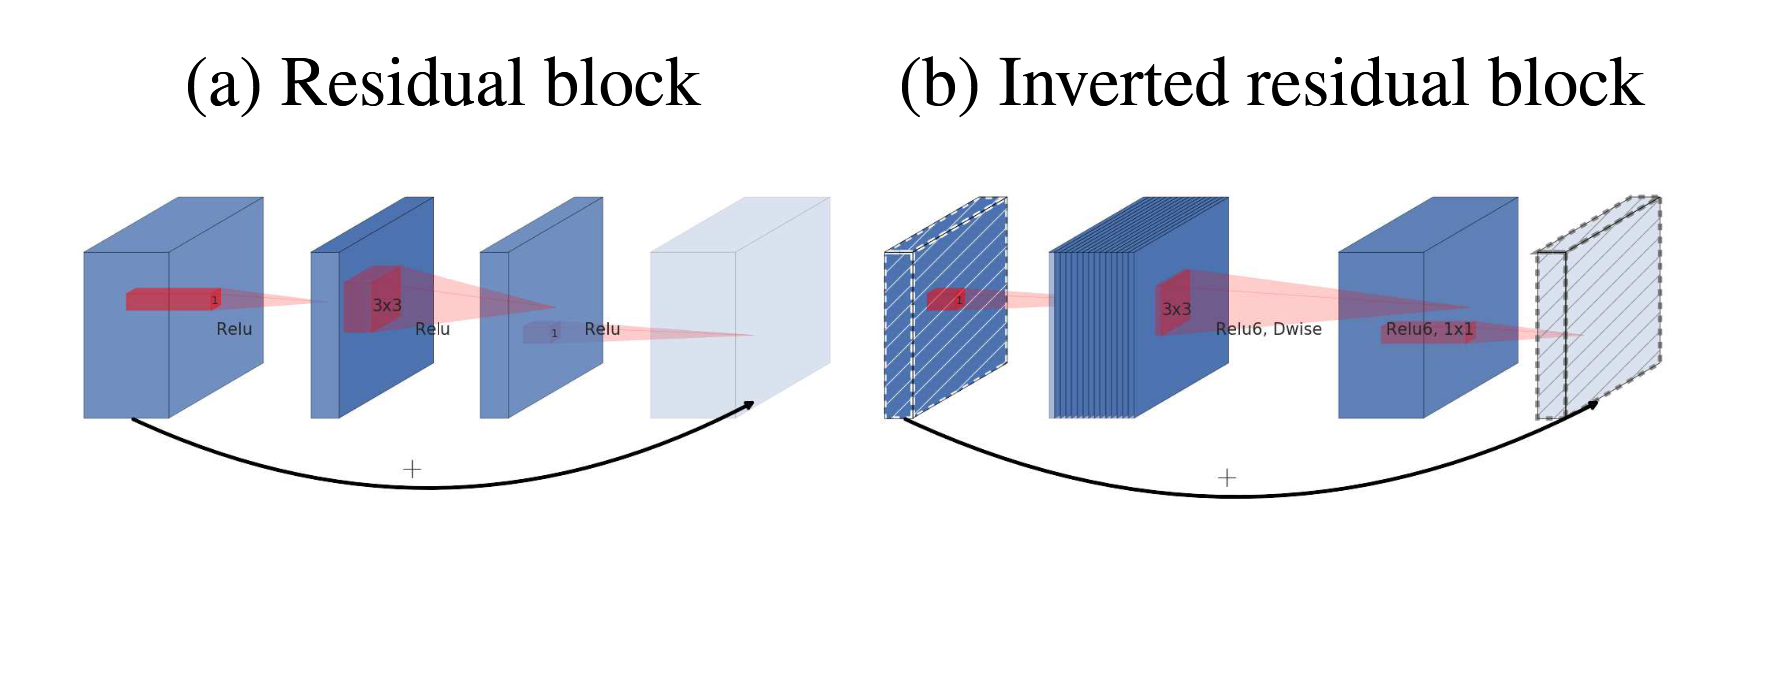
\includegraphics[width=\linewidth]{Images/Mobilenetv2.png}
        \caption{Conventional and inverted residual blocks.}
    \end{subfigure}
    \vspace{3mm}
    \caption{Original diagrams illustrating the principles underlying the two U-Net encoders. The residual learning block in (a) is reproduced from He et al. \cite{he2016resnet}; the comparison between conventional and inverted residual blocks in (b) is reproduced from Sandler et al. \cite{sandler2018mobilenetv2}. Block width in the MobileNetV2 diagram represents the relative number of channels.}
    \label{fig:resnet-mobilenet}
\end{figure}

\subsection{DeepLab Variants}

Semantic segmentation requires a model to preserve sufficiently detailed spatial information while also capturing the larger context needed to classify each image region. Conventional classification backbones gradually reduce feature-map resolution through strided convolutions and pooling, in a way that can discard spatial information that remains relevant to dense prediction. The DeepLab family addresses this aspect primarily through atrous convolution, also known as dilated convolution \cite{chen2017deeplabv3}.

Atrous convolution introduces spacing between the positions sampled by a convolutional filter. Increasing this spacing enlarges the effective field of view without increasing the number of learned kernel parameters and it can produce denser final feature maps while retaining a broad receptive field \cite{chen2017deeplabv3}. The atrous rate determines the spacing, with a rate of one corresponding to conventional convolution. DeepLabV3 applies this operation within an ASPP module. ASPP sends the encoder output through several parallel branches whose different atrous rates capture context over different spatial extents. A separate image-pooling branch summarizes the complete feature map and supplies global contextual information. The outputs are then merged to form the representation used for pixel classification \cite{chen2017deeplabv3}.

This multi-scale mechanism is relevant to Martian scene understanding,
where terrain features exhibit substantial variations in spatial scale.
Previous work has addressed this challenge by combining multi-scale
feature extraction with the preservation of local details and small
objects \cite{li2025marsseg}. These considerations motivate the use of
both broad contextual information and localized evidence in the present
work.

\begin{figure}[ht!]
    \centering
    \begin{subfigure}[t]{0.43\textwidth}
        \centering
        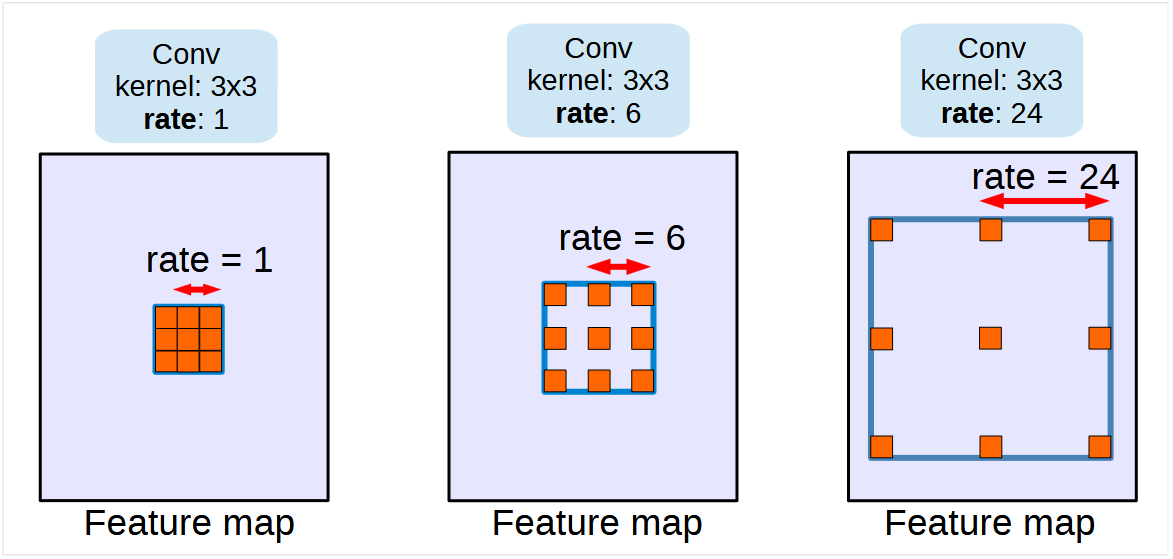
\includegraphics[width=\linewidth]{Images/deeplabv3_original_figure1.png}
        \caption{Atrous convolution at different sampling rates.}
    \end{subfigure}
    \hfill
    \begin{subfigure}[t]{0.53\textwidth}
        \centering
        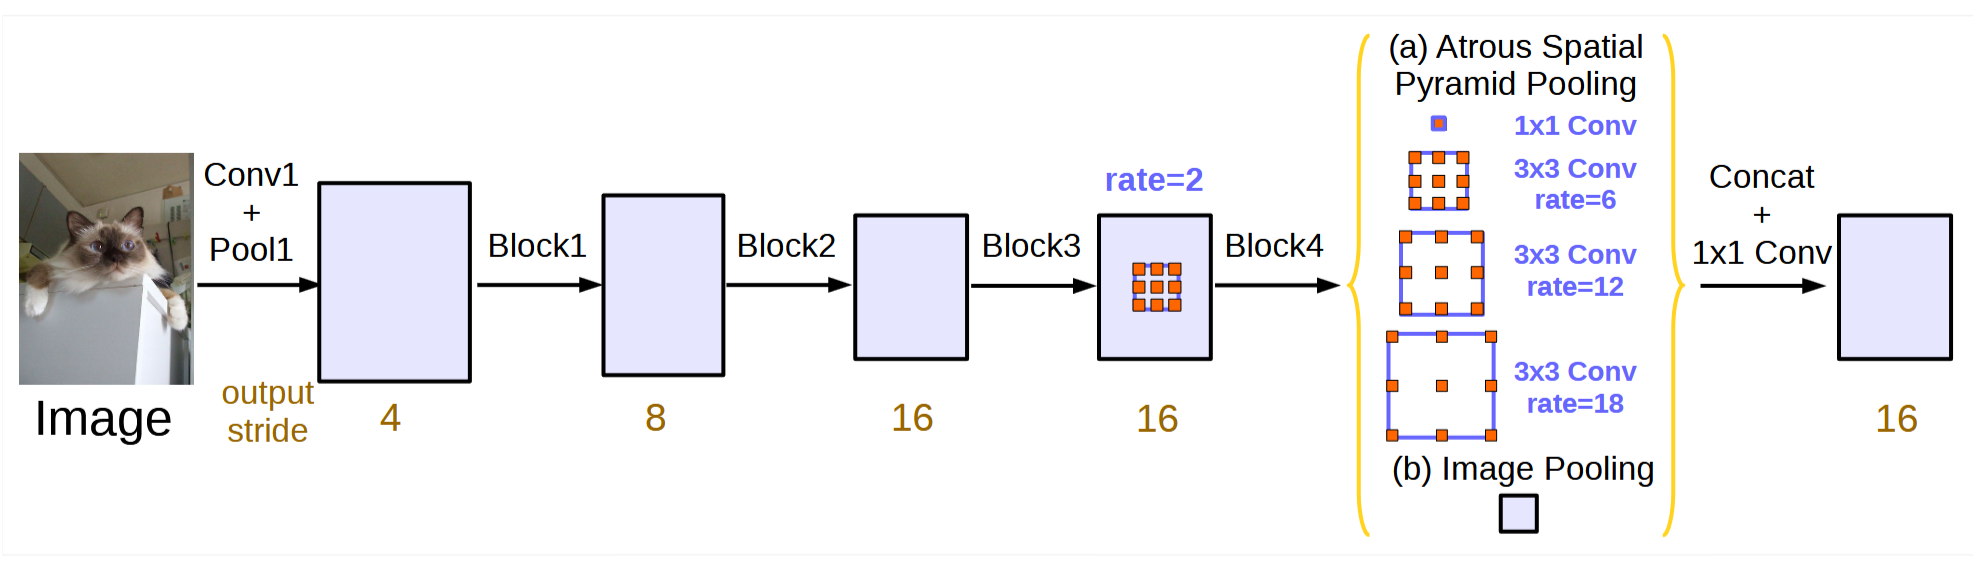
\includegraphics[width=\linewidth]{Images/deeplabv3_original_figure5.png}
        \caption{ASPP augmented with image-level features.}
    \end{subfigure}
    \vspace{3mm}
    \caption{Original diagrams illustrating the principal operations of DeepLabV3. Atrous convolution enlarges the effective field of view by changing the sampling rate, while ASPP combines parallel context branches and image-level pooling. Both diagrams are taken from Chen et al. \cite{chen2017deeplabv3}.}
\end{figure}

\paragraph{DeepLabV3 with ResNet34.}

The first variant uses ResNet34 as its encoder. Unlike U-Net, DeepLabV3 does not use a multi-stage decoder with skip connections. Instead, the ASPP features are converted into class logits and resized to the input resolution using bilinear interpolation \cite{chen2017deeplabv3}.
This variant was selected to compare two segmentation approaches built around the same backbone. U-Net--ResNet34 progressively combines encoder and decoder features to recover spatial detail, whereas DeepLabV3 gathers multi-scale context at the final encoder stage. Other architectural differences mean that this comparison does not isolate the decoder alone, but it helps examine the strengths of each approach. DeepLabV3 also provides a reference for discussing DeepLabV3+, whose additional decoder uses low-level features to refine the segmentation boundaries.

\paragraph{DeepLabV3+ with MobileNetV2.}

DeepLabV3+ extends the predecessor by combining its multi-scale contextual encoder with a lightweight decoder \cite{chen2018deeplabv3plus}. The ASPP representation is first upsampled and then merged with an earlier feature map from the backbone, providing information that can support the refinement of object and region boundaries. The fused features are processed by the decoder before a final upsampling operation restores the prediction to the input resolution.

The resulting architecture combines two complementary mechanisms. Atrous convolution and ASPP encode contextual information over several spatial ranges, while the decoder reintroduces higher-resolution information that is less accessible from the deepest feature map alone. The original DeepLabV3+ study further employed depthwise-separable convolutions within the ASPP and decoder modules to reduce their computational cost \cite{chen2018deeplabv3plus}.

\begin{figure}[ht!]
    \centering
    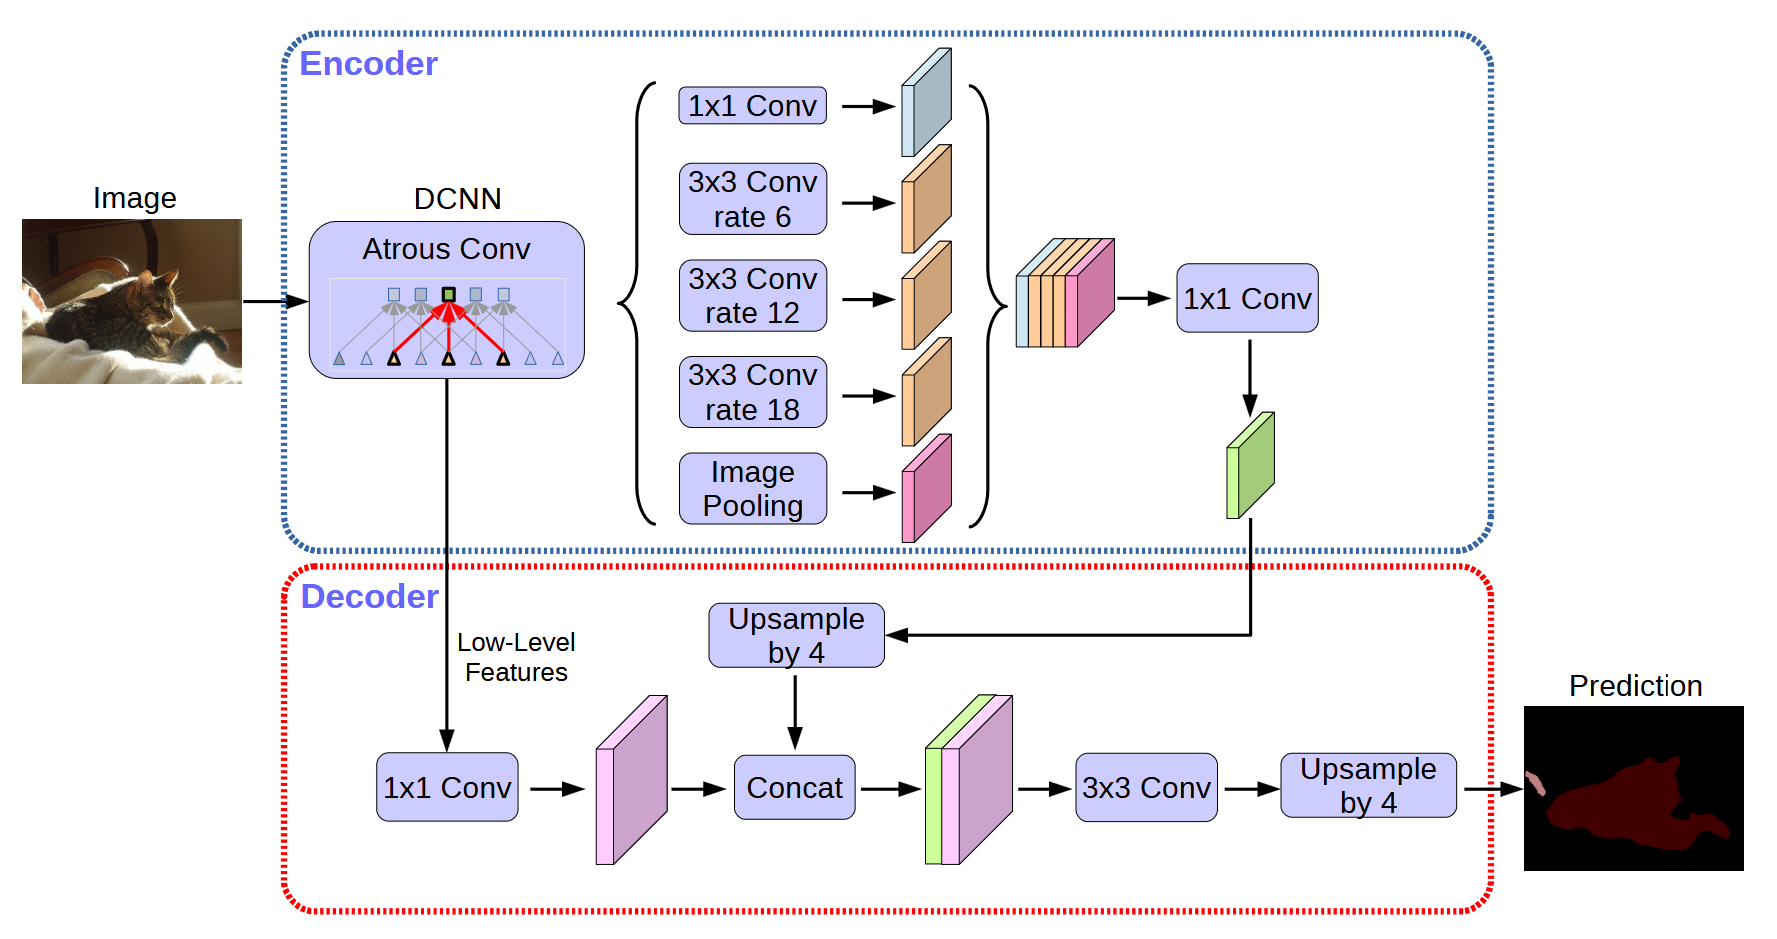
\includegraphics[width=0.9\textwidth]{Images/deeplabv3plus_original_figure2.png}
    \vspace{3mm}
    \caption{Original DeepLabV3+ architecture, Reproduced from Chen et al. \cite{chen2018deeplabv3plus}.}
\end{figure}

The second variant makes use of the same MobileNetV2 backbone utilized by the previous U-Net configuration, providing a second cross-family point of comparison. This choice produces a deployment-oriented configuration of DeepLabV3+ rather than reproducing the modified Xception backbone emphasized in the original paper.

\subsection{SegFormer-B0}

SegFormer combines a hierarchical Transformer encoder, called Mix Transformer (MiT), with a lightweight multilayer perceptron (MLP) decoder \cite{xie2021segformer}. The architecture was included to examine an attention-based alternative to the convolutional models described above.

Self-attention allows each position to gather information from distant parts of the image within a single layer, whereas local convolutions build larger context through successive layers \cite{vaswani2017attention}. For Martian semantic segmentation, this provides a reason to investigate whether relationships across an image can help discriminate terrain regions whose local appearance may be ambiguous.
MiT extracts features in four stages, producing progressively larger representations. Overlapping patch embeddings preserve local continuity, while attention uses spatially reduced features to lower its computational cost. Each block also includes a Mix-FFN module, which adds local spatial information through a depthwise convolution. This removes the need for explicit positional embeddings and their interpolation when the input resolution changes \cite{xie2021segformer}.

The decoder projects the four encoder outputs into a common feature dimension, resizes them to the same spatial resolution, and fuses them before classification \cite{xie2021segformer}. This brings all encoder stages together in a single fusion step, and its evaluation therefore examines whether this compact decoder can preserve the spatial detail needed for terrain segmentation.

\begin{figure}[ht!]
    \centering
    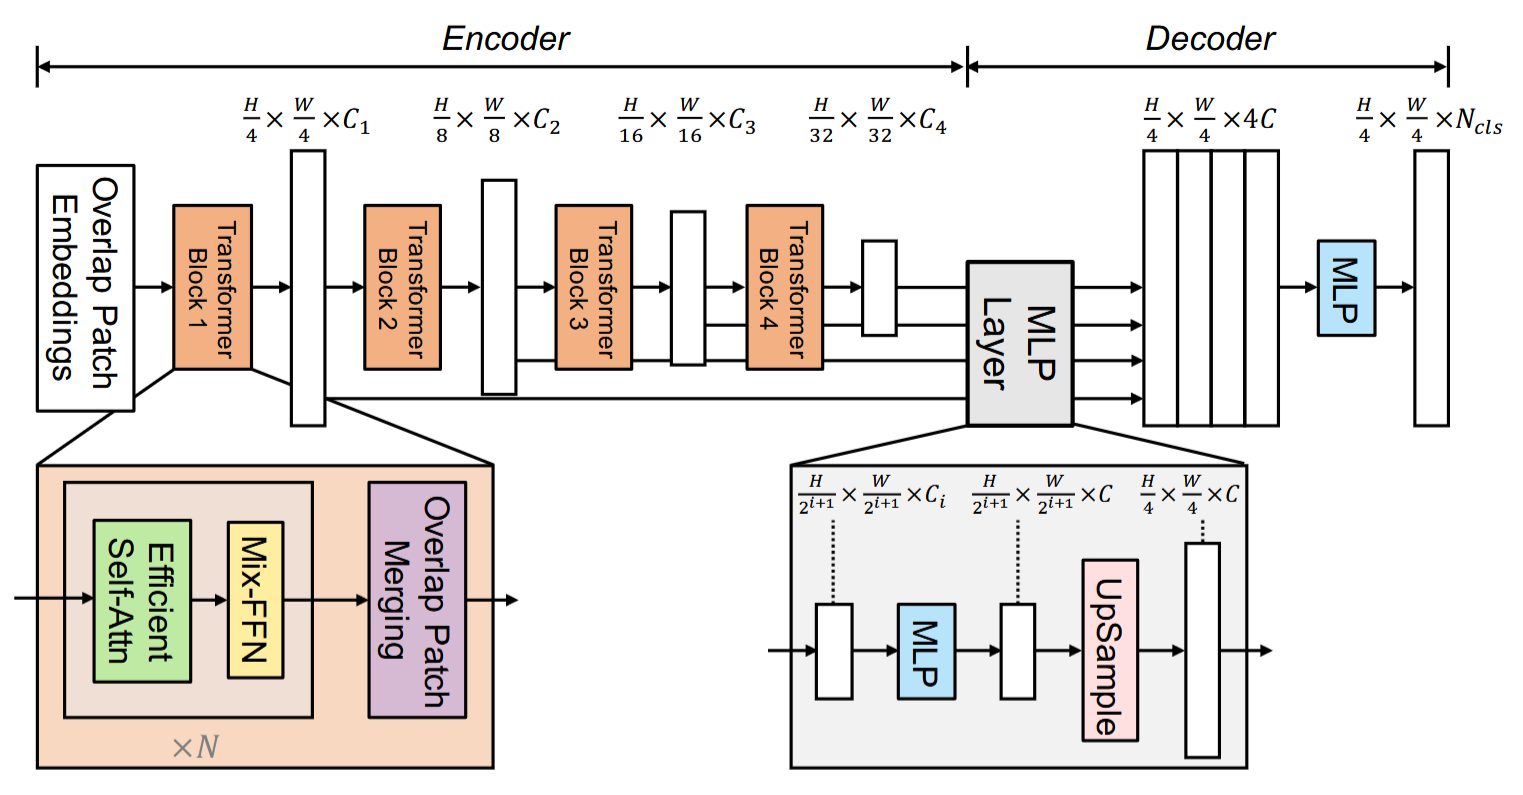
\includegraphics[width=\textwidth]{Images/segformer_original_figure2.png}
    \vspace{3mm}
    \caption{Original SegFormer architecture, showing the hierarchical Transformer encoder and the decoder that fuses its outputs. Reproduced from Xie et al. \cite{xie2021segformer}.}
\end{figure}

SegFormer was included because it is one of the model families evaluated in Mars-Bench \cite{purohit2025marsbench}. B0, its smallest variant, was selected to limit model size \cite{xie2021segformer}, while testing its accuracy-efficiency trade-off, with results presented in the evaluation chapter.

\subsection{LCNet Variants}

The Lightweight Context-Aware Network (LCNet) was introduced by Shi et al. to address the computational costs of semantic segmentation through partial-channel processing and a compact encoder-decoder design \cite{shi2024lcnet}. LCNet was included in this study to extend the architectural comparison toward models explicitly designed to limit computational cost, in addition to the architecture families considered in Mars-Bench. Its inclusion allows the study to investigate whether a smaller network could provide sufficient accuracy for Martian scene understanding.

\begin{figure}[htbp]
    \centering
    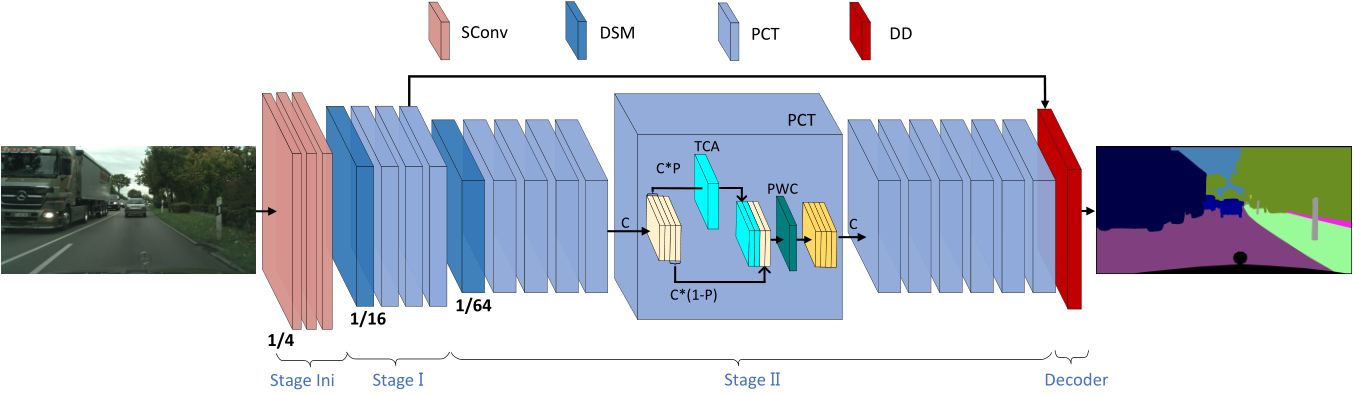
\includegraphics[width=\textwidth]{Images/LCNet.png}
    \caption{Overview of the LCNet architecture.
        Original diagram provided by the authors of \cite{shi2024lcnet}.}
    \label{fig:lcnet-architecture}
\end{figure}

Its main processing unit is the Partial-Channel Transformation (PCT) block, which splits the input features into two groups. One group passes directly to the output fusion, while the other undergoes context processing. The two groups are then concatenated and combined through a pointwise convolution \cite{shi2024lcnet}. In the project implementation, each path receives half of the channels, limiting the amount of spatial processing while retaining information from both groups. The transformed group is processed by a Three-Branch Context Aggregation (TCA) module, where a standard convolution first produces intermediate features, which are then processed by local and dilated depthwise convolutions. Their outputs are added to the intermediate features, combining information from nearby positions and wider regions without further downsampling.

\begin{figure}[htbp]
    \centering
    \begin{minipage}[c]{0.48\textwidth}
        \centering
        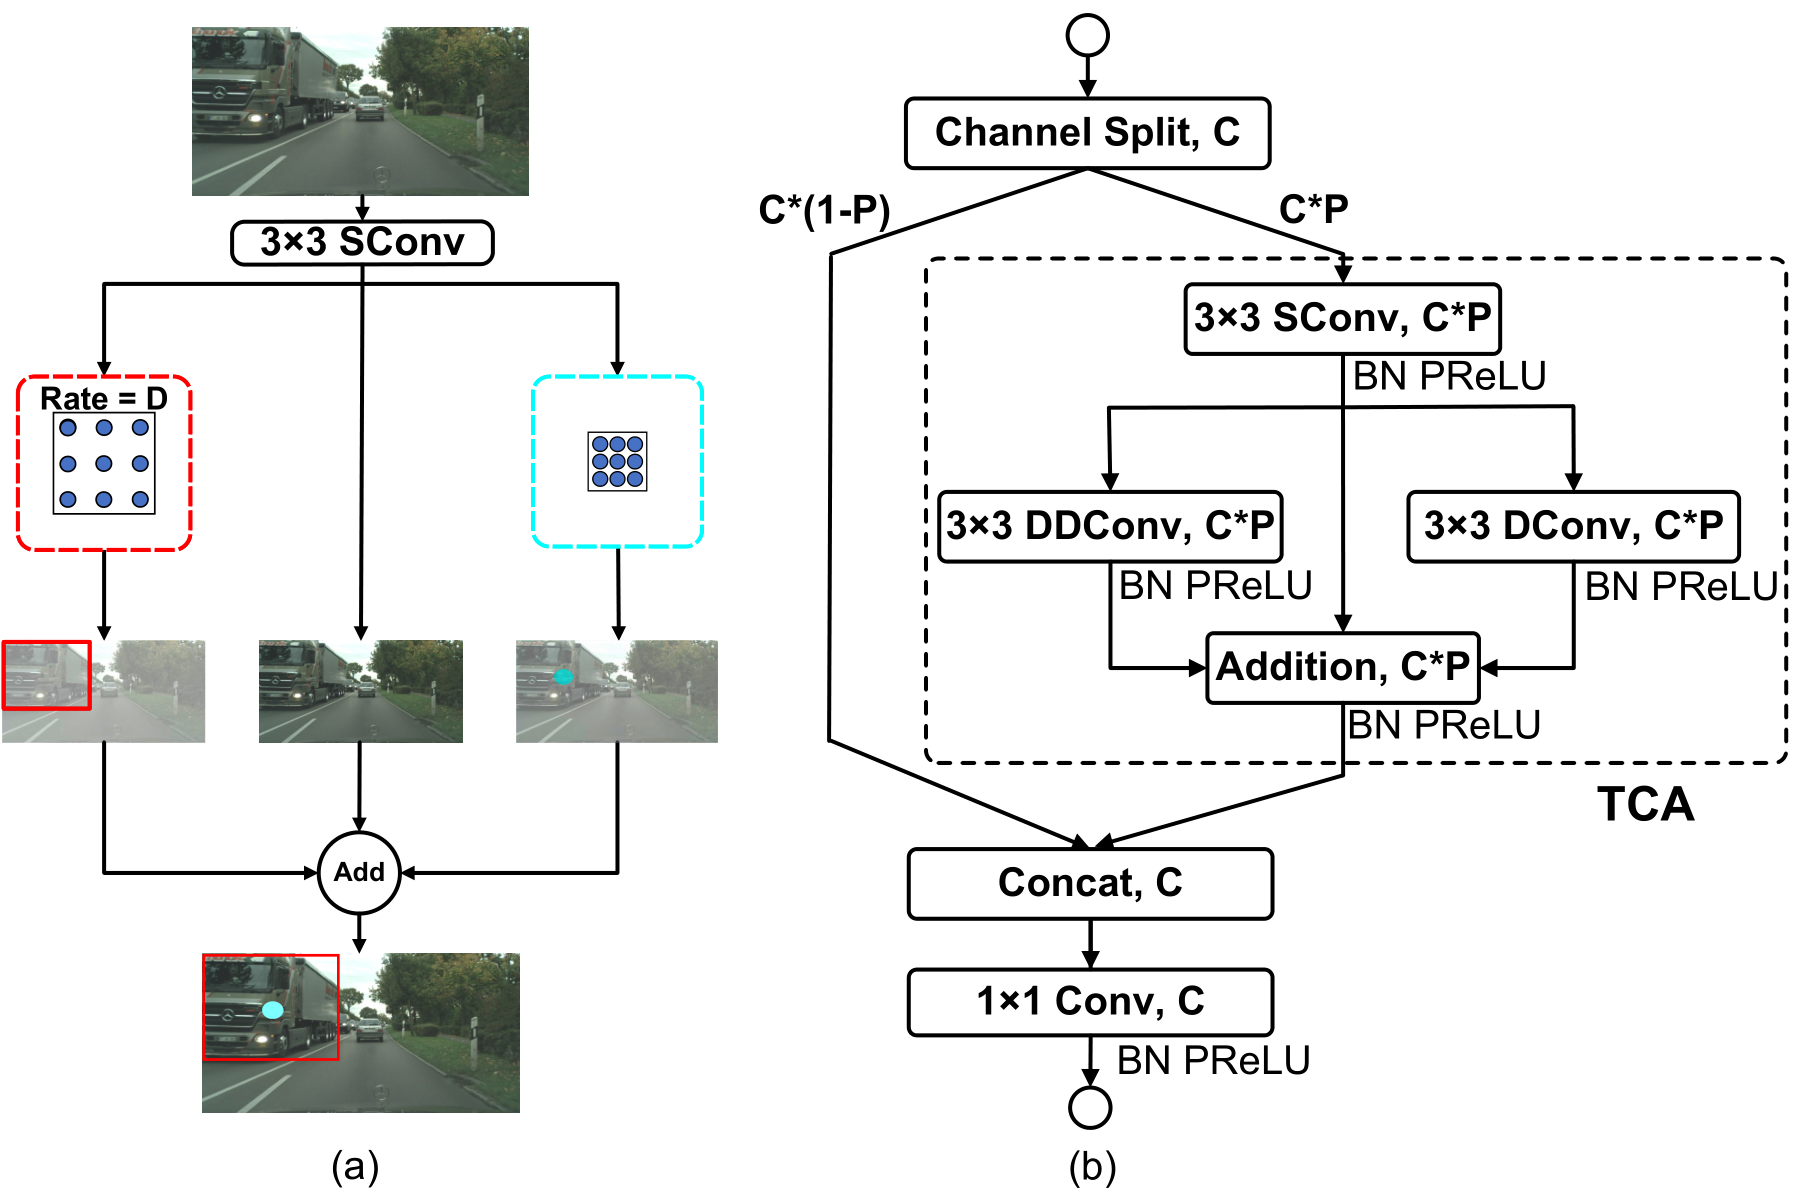
\includegraphics[width=\linewidth]{Images/lcnet_pct.png}
    \end{minipage}
    \hfill
    \begin{minipage}[c]{0.48\textwidth}
        \centering
        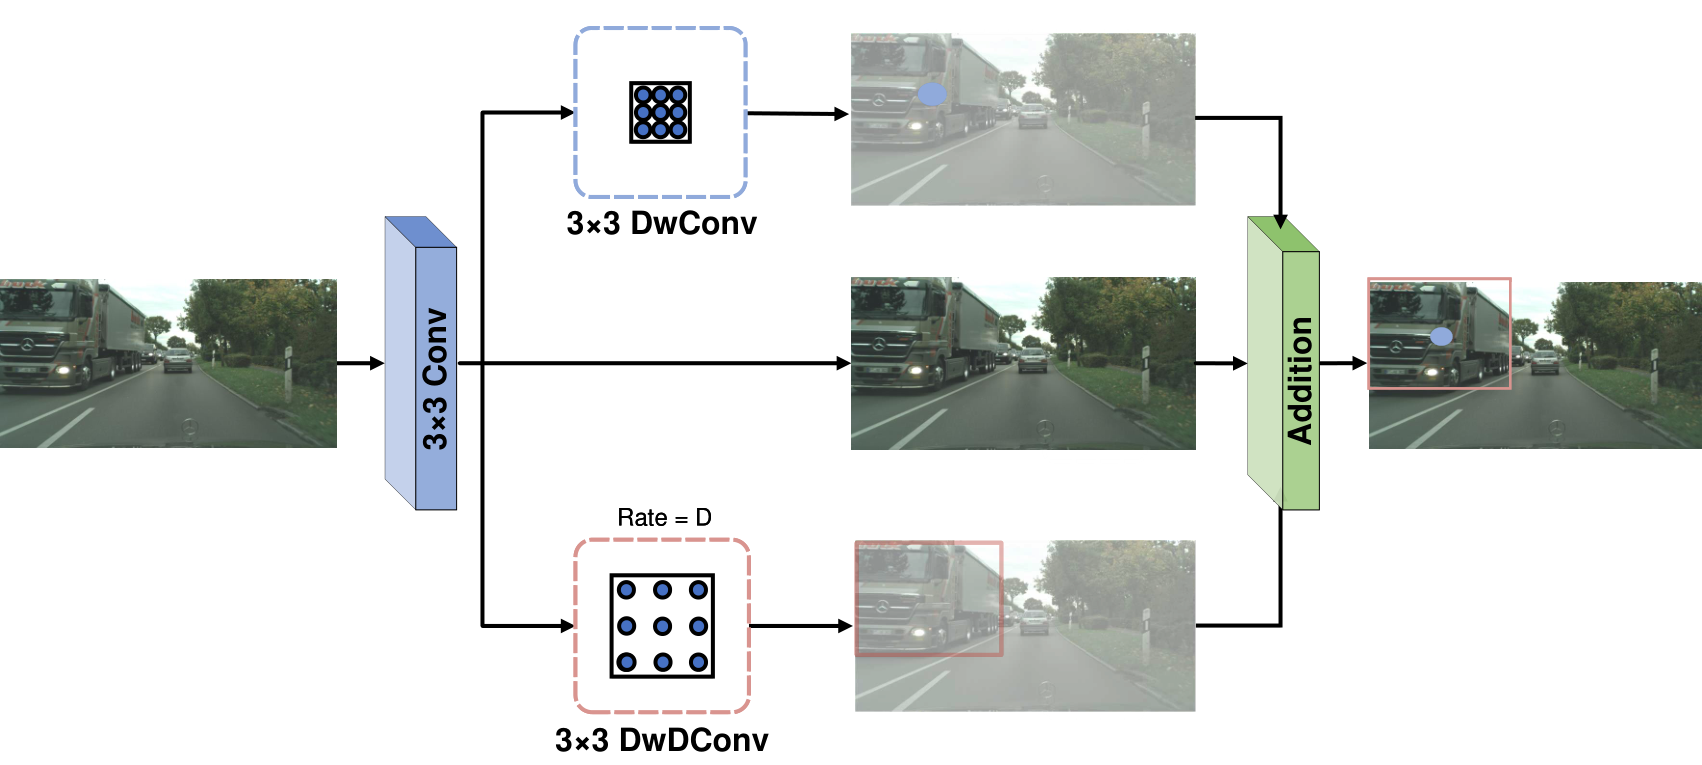
\includegraphics[width=\linewidth]{Images/lcnet_tca.png}
    \end{minipage}
    \caption{Partial-channel transformation (left) and three-branch
        context aggregation (right). Original diagrams provided by the
        authors of \cite{shi2024lcnet}.}
    \label{fig:lcnet-pct-tca}
\end{figure}

The encoder contains an initial convolutional stage followed by two PCT stages. Each PCT stage begins with a downsampling block that combines a strided convolution with max pooling, so most context processing takes place at reduced spatial resolutions. The decoder then brings together features from both stages through two attention mechanisms \cite{shi2024lcnet}. The shallower features provide spatial guidance, while the deeper features are refined through a reverse-guidance branch. After resizing the deeper features, the decoder combines them with the spatial guidance through element-wise multiplication. A depthwise convolution and a pointwise classifier produce the class scores, which are resized to the input resolution using bilinear interpolation.

Two configurations were implemented: LCNet\(_{3,7}\) and LCNet\(_{3,11}\). Both use three PCT blocks in the first encoder stage, followed by seven and eleven blocks in the second stage, respectively. LCNet\(_{3,11}\) therefore adds four context-processing blocks without changing the overall design, allowing the comparison to examine whether a deeper encoder offers enough additional accuracy to justify its computational cost. Both variants were independently reimplemented for the project and configured to predict the nine S5Mars classes, using the random initialization described above.

\subsection{Architectural Comparison}

Table~\ref{tab:segmentation-architecture-static-comparison} compares the seven configurations independently of their predictive performance. Parameter counts refer to the nine-class implementations used for S5Mars and include all trainable layers, while R34 and MV2 denote ResNet34 and MobileNetV2, respectively.

\begin{table}[ht!]
    \centering
    \small
    \resizebox{\linewidth}{!}{%
        \begin{tabular}{@{}l l l r r@{}}
            \toprule
            \textbf{Model}          &
            \textbf{Encoder}        &
            \textbf{Initialization} &
            \textbf{Params. (M)}                 \\
            \midrule
            \midrule
            U-Net
                                    & R34
                                    & ImageNet
                                    & 24.438     \\

            U-Net
                                    & MV2
                                    & ImageNet
                                    & 6.630      \\

            DeepLabV3
                                    & R34
            \linebreak
                                    & ImageNet
                                    & 26.009     \\

            DeepLabV3+
                                    & MV2
                                    & ImageNet
                                    & 4.381      \\

            SegFormer-B0
                                    & MiT-B0
                                    & ADE20K
                                    & 3.716      \\

            LCNet\(_{3,7}\)
                                    & LCNet stem
                                    & Random
                                    & 0.509      \\

            LCNet\(_{3,11}\)
                                    & LCNet stem
                                    & Random
                                    & 0.729      \\
            \bottomrule
        \end{tabular}
    }
    \vspace{5mm}
    \caption{Comparison of the segmentation architectures implemented for the nine-class S5Mars task. }
    \label{tab:segmentation-architecture-static-comparison}
\end{table}

\section{Training}

The segmentation models share a configurable training pipeline that controls the optimization procedure, loss function, data sampling, and checkpoint selection. A common reference configuration provides shared optimization settings across the architecture families, while allowing individual components to be modified for the ablation studies. The U-Net, DeepLab, and SegFormer configurations were trained for 30 epochs, whereas the two LCNet configurations were trained for 60 epochs. Training used a batch size of 32, with images processed at the \(512 \times 512\) resolution defined in the preprocessing section. The pretrained models are fine-tuned end to end, therefore all network parameters remain trainable throughout optimization, including the encoders initialized from pretrained weights, whereas the LCNet configurations are optimized from random initialization. The training images are shuffled at every epoch, while validation and test samples are processed without shuffling or stochastic augmentation.

The loss function combines pixel-wise cross-entropy (CE) with Generalized Dice Loss (GDL):
\begin{equation}
    \mathcal{L}
    =
    \alpha \mathcal{L}_{\mathrm{CE}}
    +
    (1-\alpha)\mathcal{L}_{\mathrm{GDL}},
    \qquad \alpha = 0.5.
    \label{eq}
\end{equation}
Cross-entropy supervises the probability assigned to the target class at each pixel, whereas the Dice component measures agreement between the predicted probability maps and the target regions. Generalized Dice introduces class-dependent weighting to account for differences in region size, following the formulation investigated by Sudre et al. for imbalanced segmentation tasks \cite{sudre2017generalizeddice}. Combining the two terms therefore provides pixel-wise classification supervision alongside a region-overlap objective. This follows the rationale to combine the gradient stability of cross-entropy with the ability of Dice-based losses to handle class imbalance \cite{yeung2022unified}.

In the implemented Generalized Dice loss, class volumes are computed from the target masks across the current mini-batch. Classes present in the batch receive weights inversely proportional to the square of their pixel counts, while absent classes receive zero weight in the Dice calculation. These weights are recomputed for each batch rather than derived from precomputed class frequency scores. A smoothing constant of \(10^{-5}\) is added to the numerator and denominator of the overlap ratio. The pipeline also supports a single loss function alone and alternative Dice weighting schemes. The available configurations include inverse-volume weighting or uniform weights over the classes present in the batch. These alternatives allow the contribution of the loss formulation to be examined separately from changes in architecture.

The Optimizer is AdamW \cite{loshchilov2019adamw}, with a base learning rate of \(10^{-4}\) and a weight-decay coefficient of \(10^{-2}\). A linear warm-up during the first epoch is followed by cosine decay toward zero over the remaining epochs, without warm restarts \cite{loshchilov2017sgdr}. Training runs for the fixed epoch budget without early stopping, while the checkpoint with the best validation performance is retained for evaluation. Training was performed on Kaggle using two NVIDIA T4 GPUs, each with 16 GB of VRAM.

\paragraph{Training-data sampling and optional augmentation.}

Standard sampling is the default configuration, while image oversampling is available as a separate training-only option. Unlike the class weighting inside Generalized Dice, which depends on pixel counts within a batch, oversampling uses the class frequency of the training images. It therefore modifies how frequently images are presented to the model without changing their masks or the loss definition. When oversampling is enabled, the number of training images containing each class is first computed. Each image receives the largest rarity factor among its eligible classes, where the rarity factor is the square root of the ratio between the most frequent class count and the count of the class under consideration. In the oversampling experiments reported in this thesis, the image weights were capped at 6 before normalization, and images were sampled with replacement. With the reference epoch-length multiplier of 1, the number of samples equals the number of training images, preserving the nominal training length although some images may be repeated and others omitted in an epoch.
Geometric augmentation is controlled independently from sampling and remains disabled in the default configuration. When enabled, the transformations described in the preprocessing section are applied jointly to each training image and its mask. Neither augmentation nor oversampling modifies the validation or test distributions.

\begin{table}[ht!]
    \centering
    \begin{tabular}{@{}l c@{}}
        \toprule
        \textbf{Setting}                     & \textbf{Default configuration}     \\
        \midrule
        \midrule
        Input resolution                     & \(512 \times 512\)                 \\
        Training epochs                      & 30 (60 for LCNet)                  \\
        Batch size                           & 32                                 \\
        Trainable parameters                 & Entire network                     \\
        Optimizer                            & AdamW                              \\
        Base learning rate                   & \(10^{-4}\)                        \\
        Weight decay                         & \(10^{-2}\)                        \\
        Learning-rate schedule               & Linear warm-up and cosine decay    \\
        Warm-up duration                     & 1 epoch                            \\
        Loss Function                        & Cross-entropy and Generalized Dice \\
        Cross-entropy coefficient \(\alpha\) & 0.5                                \\
        Dice class weighting                 & Inverse-square batch volume        \\
        Image-level oversampling             & Disabled                           \\
        Training augmentation                & Disabled                           \\
        Checkpoint selection                 & Highest validation mIoU            \\
        \bottomrule
    \end{tabular}
    \vspace{5mm}
    \caption{Reference configuration for semantic-segmentation training.
        Experiment-specific changes to the loss, sampling, or augmentation
        settings are reported with the corresponding evaluations.}
    \label{tab}
\end{table}

\section{Evaluation Metrics}
\label{sec:segmentation-evaluation-metrics}

Segmentation performance is evaluated using Pixel Accuracy (PA), per-class Intersection over Union (IoU), and mean Intersection over Union (mIoU), following established semantic-segmentation evaluation practice \cite{long2015fcn}. Predictions are obtained by selecting the highest-scoring class at each pixel, and the metrics are computed from a confusion matrix accumulated over the entire evaluated partition rather than averaged across images or mini-batches.

Let \(TP_c\), \(FP_c\), and \(FN_c\) denote the true-positive, false positive, and false-negative pixel counts for class \(c\). The metrics are defined as
\begin{equation}
    \begin{aligned}
        \mathrm{Pixel\ Accuracy}
         & = \frac{\sum_c TP_c}{N},           \\
        \mathrm{IoU}_c
         & = \frac{TP_c}{TP_c + FP_c + FN_c}, \\
        \mathrm{mIoU}
         & = \frac{1}{|\mathcal{C}_{+}|}
        \sum_{c \in \mathcal{C}_{+}} \mathrm{IoU}_c,
    \end{aligned}
    \label{eq:segmentation-evaluation-metrics}
\end{equation}
where \(N\) is the total number of evaluated pixels and \(\mathcal{C}_{+}\) contains the classes present in the ground truth of the evaluated partition.

PA measures the overall proportion of correctly classified pixels, but consequently gives greater influence to classes occupying larger image regions. In contrast, mIoU assigns equal weight to each included class and serves as the primary checkpoint-selection metric. Per-class IoU complements this aggregate measure by exposing differences between semantic categories that a single score may conceal.

% Computational efficiency is assessed separately through parameter count, estimated FLOPs, inference latency, and frames per second (FPS), with the hardware and measurement conditions specified in the evaluation chapter.

\section{Optimization and Quantization}
\label{sec:optimization-quantization}

Quantization was investigated to test the efficiency of the segmentation models for resource-constrained deployment, with the objective of reducing model storage and inference costs while preserving segmentation accuracy. Selected FP32 checkpoints were exported to the Open Neural Network Exchange (ONNX) format as full  models, alongside FP16 variants obtained by converting eligible parameters and operations to half precision while maintaining FP32 inputs and outputs.

Static Post-Training Quantization (PTQ) to INT8 was applied without retraining the models. The PTQ configuration used entropy-based calibration with 500 images randomly sampled from the training split, without using their segmentation annotations. Selected weights and activations used symmetric quantization, with per-channel quantization for weights and per-tensor quantization for activations. The quantized models used the ONNX Quantize/Dequantize (QDQ) format, which introduces explicit nodes to represent conversions between floating point values and their quantized representations \cite{onnxruntimeQuantization}.

An alternative INT8 strategy used Quantization-Aware Training (QAT) with NVIDIA ModelOpt. Fake-quantization operations simulated rounding and clipping during fine-tuning, allowing the models to adapt to quantization effects \cite{jacob2018quantization}. The training objective combined the supervised segmentation loss with knowledge distillation from a frozen FP32 teacher, with coefficients of 0.7 and 0.3, respectively. Distillation used Kullback-Leibler divergence between softened class-probability maps, with the divergence scaled by the squared temperature. The resulting models were exported to ONNX with explicit quantization and dequantization operations, without an additional PTQ step.

The ModelOpt fine-tuning configuration used a maximum of 10 epochs, a mini-batch size of 2, AdamW with a learning rate of \(10^{-5}\) and weight decay of \(10^{-2}\), with one epoch of linear warm-up followed by cosine decay. The checkpoint with the highest validation mIoU was kept, with early stopping applied after three epochs without improvement.

Both INT8 strategies used selective quantization, keeping floating-point computations where required for compatibility or accuracy. For example, in the evaluated Conv-only configuration of SegFormer-B0, INT8 was restricted to convolutional layers, whereas linear projections, attention matrix multiplications, normalization, and softmax remained in floating point, with FP16 fallback in TensorRT. The resulting models therefore used mixed precision rather than an entirely integer computation graph.
%ONNX FP32 and FP16 inference used ONNX Runtime with its CUDA execution provider. PTQ INT8 inference used its TensorRT execution provider, with CUDA and CPU fallback, whereas ModelOpt QAT models were executed directly with TensorRT.
Quantization configurations were selected using the validation split, reserving the test split for final evaluation.

\chapter{Synthetic Dataset Generation}
%Curiosity's wheel perforations are monitored through manual image inspections \cite{nasa2016wheelinspection,rankin2022wheelassessment}, motivating automated methods for damage detection and localization.


\section{Design Requirements}
The dataset was designed to contain RGB views covering all six wheel positions of a Curiosity Rover model, with one designated target wheel in each image. The anomaly class was restricted to localized through-holes in the wheel skin, with variations in shape, size, and position. Broken grousers and other failure modes remained outside the scope of this work. Normal samples were defined by the absence of an injected perforation so that dust and non-anomalous surface wear could remain part of the normal visual distribution.

The annotation requirements reflected the distinction between detecting damage and localizing it. Each sample required an image-level condition label and a target-wheel mask, while anomalous samples additionally required a binary mask identifying the damage region. The training split was required to contain only normal samples, whereas validation and test included both normal and damaged conditions. For evaluation, paired clean and damaged images were generated with the same camera, wheel pose, lighting, and surface-wear parameters, allowing direct comparisons in which the only difference was the introduced perforation. Each pair had to remain inside a single split to prevent paired scene leakage. Coverage of camera viewpoints, wheel rotations, illumination, and benign wear was required to avoid evaluating inspection under a single fixed appearance.

These requirements define a controlled synthetic benchmark for visible wheel perforations, used to evaluate how efficiently the proposed approaches tackle the task.

\section{Asset Preparation}
Asset preparation focused on visually representing Curiosity and recreating its Martian surroundings as faithfully as possible, while keeping the scene suitable for controlled, wheel-specific modifications. The three-dimensional scene was assembled in Blender, which was used to prepare the rover and terrain assets and render the synthetic images.

\paragraph{Rover model.}
The rover asset was based on the publicly available Curiosity model distributed by NASA's Visualization Technology Applications and Development team \cite{nasa2019curiositymodel}. Using an existing model avoided reconstructing the vehicle from photographs and provided both the wheel geometry and the surrounding rover structure. Retaining this context was important because the chassis and suspension contribute to the appearance of inspection images through occlusions and shadows.

After importing the model into Blender, the six wheels were separated into independently addressable objects, while the remaining vehicle structure was retained as an assembly. This organization enabled wheel-specific damage generation, rotation control, and mask extraction without rebuilding the rover geometry. The model was used for visual image generation rather than as an engineering representation of the rover's mechanical behavior.

\paragraph{Martian environment.}
The terrain was derived from observations of Gale Crater acquired by the High Resolution Imaging Science Experiment (HiRISE), using a digital terrain model and associated orthorectified imagery \cite{hirisegaleterrain}. These products provided a real observation-based foundation for the environment, including variations in elevation and surface appearance. A common region was extracted from both products, with the elevation data converted into a terrain mesh at metric scale and the corresponding imagery mapped onto its surface.

The orbital data were not detailed enough for close-up wheel views, so a local procedural terrain patch was added with grains, rocks, and small surface irregularities. Material effects provided finer visual detail without adding geometry, while rock models were reused to keep the scene manageable. These additions complemented the real terrain data but did not reproduce the exact ground surface at the site. Figure~\ref{fig:rover-terrain-scene} shows the rover asset and the surrounding terrain assembled in Blender for synthetic image generation.

\begin{figure}[ht!]
    \centering
    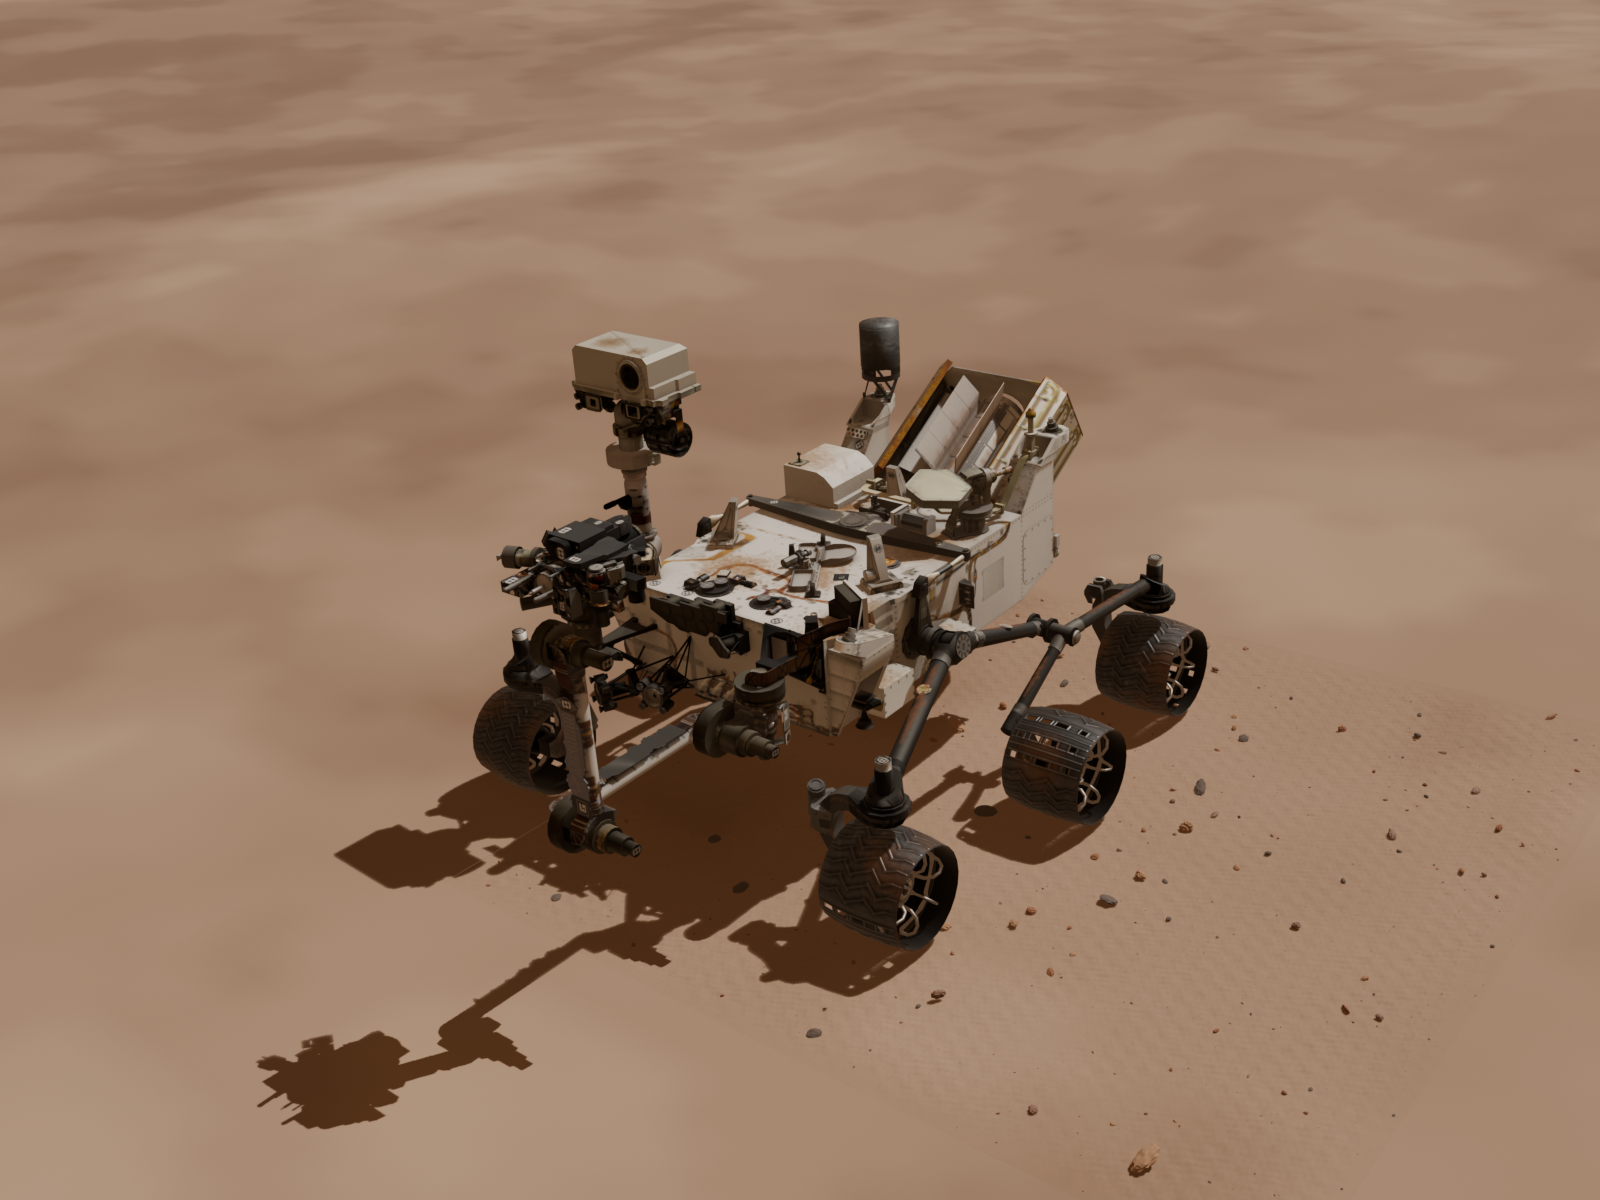
\includegraphics[width=0.70\textwidth]{Images/rover_terrain_overview_v2.png}
    \caption{Overview of the Blender scene, showing the Curiosity rover
        asset and the surrounding terrain used for synthetic image generation.}
    \label{fig:rover-terrain-scene}
\end{figure}

\section{Synthetic Damage Generation}
\label{sec:synthetic-damage-generation}
Damage generation focused on a single anomaly class: through-holes in the wheel surface, with each anomalous image containing one injected hole on the designated target wheel. Hole contours were generated procedurally using three profile families: jagged slits, branched tears, and peeled-window profiles. Variations in contour irregularity, orientation, and dimensions provided different realizations within each family. Three size-based severity levels were defined, denoted small, medium, and large, with their length sampled within 2.7-4.1\,cm, 4.4-6.8\,cm, and 7.3-11.6\,cm, respectively. These categories describe the generated geometry rather than a mechanical assessment of wheel health. Figure~\ref{fig:damage-severity} shows an example of each level.

\begin{figure}[ht!]
    \centering
    \begin{minipage}[b]{0.32\textwidth}
        \centering
        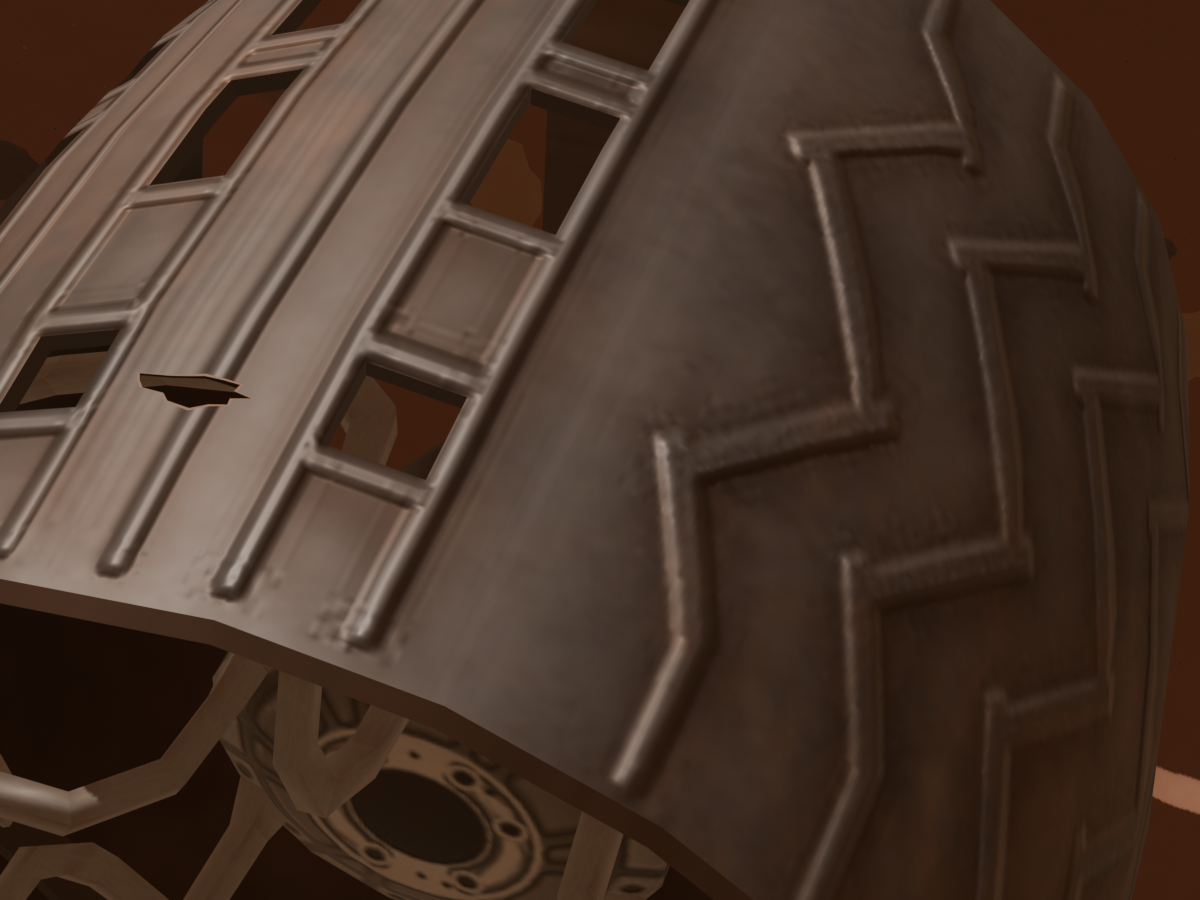
\includegraphics[width=\linewidth]{Images/hole_severity_small.png}
        \par\smallskip
        {\small (a) Small}
    \end{minipage}
    \hfill
    \begin{minipage}[b]{0.32\textwidth}
        \centering
        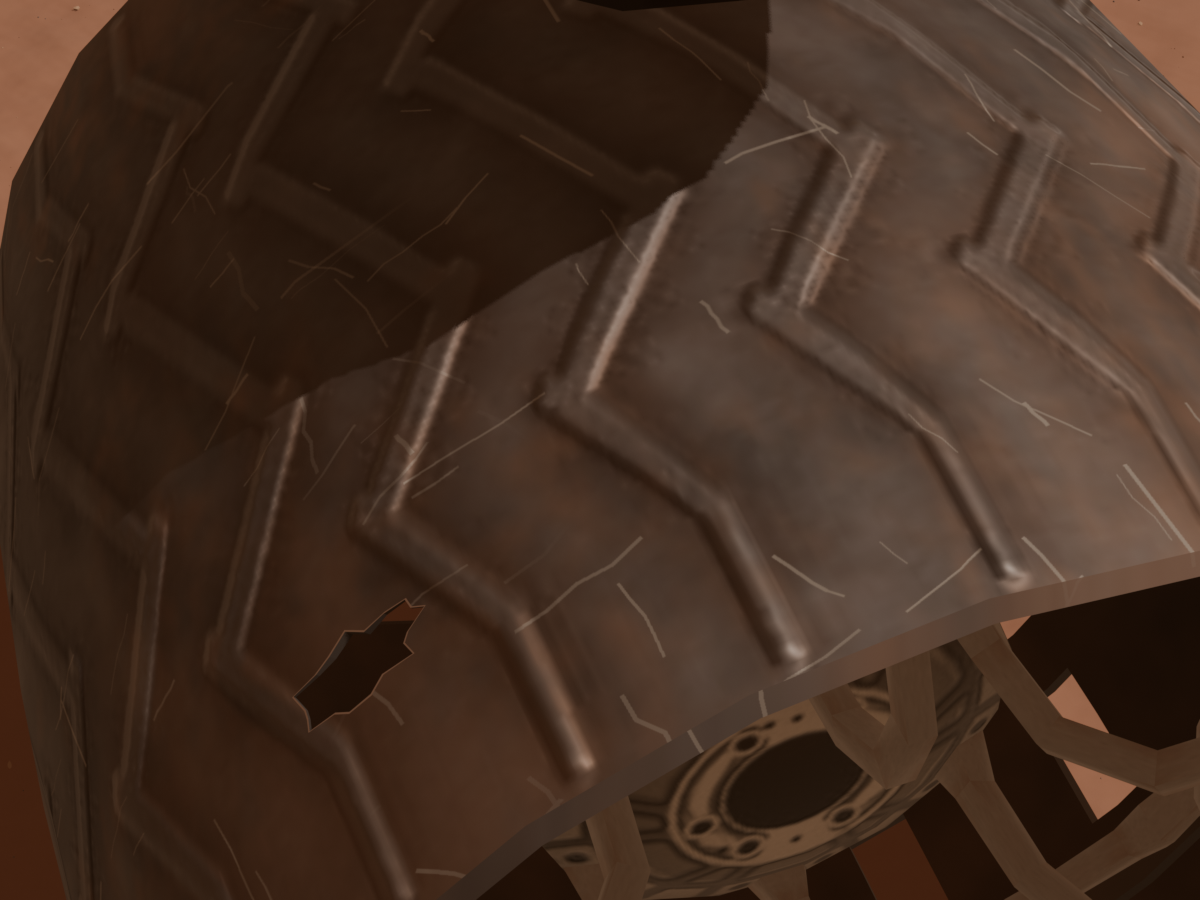
\includegraphics[width=\linewidth]{Images/hole_severity_medium.png}
        \par\smallskip
        {\small (b) Medium}
    \end{minipage}
    \hfill
    \begin{minipage}[b]{0.32\textwidth}
        \centering
        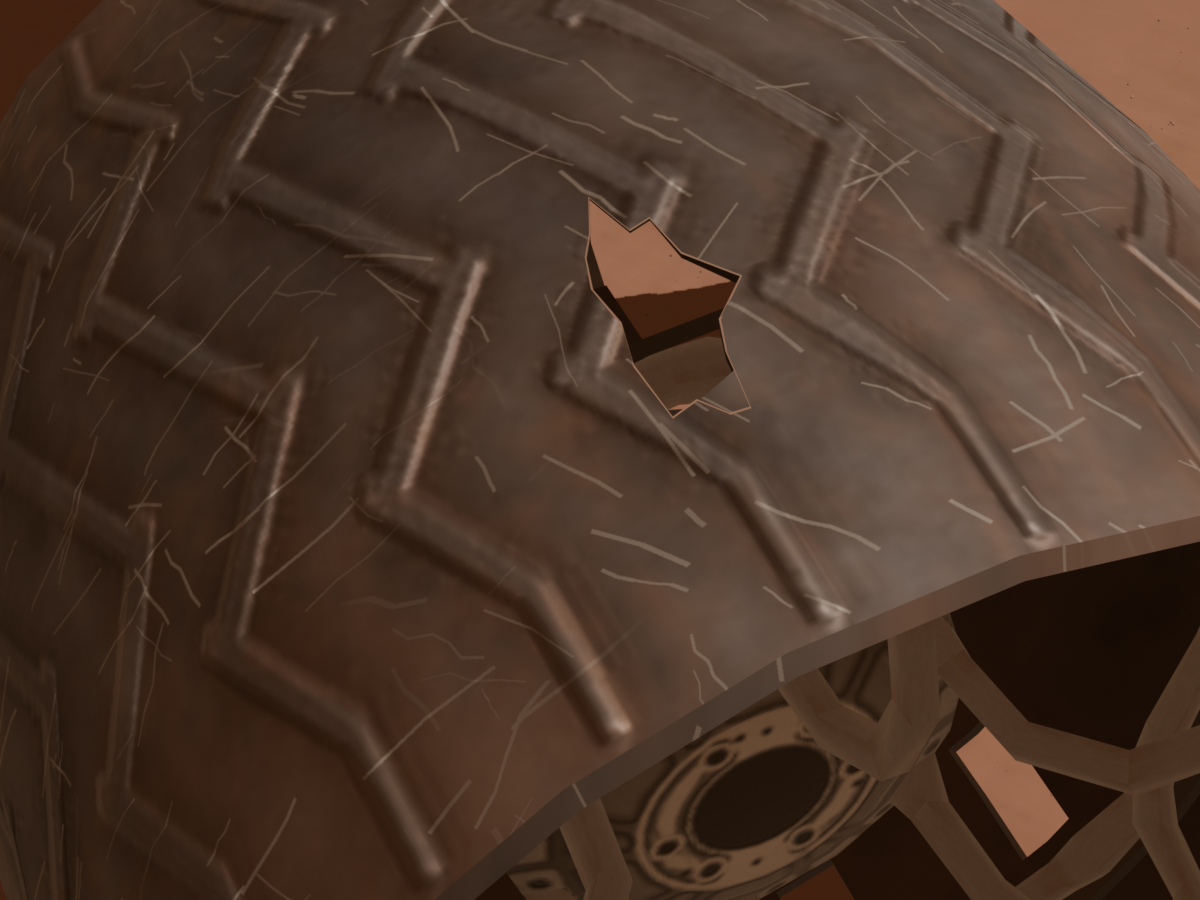
\includegraphics[width=\linewidth]{Images/hole_severity_large.png}
        \par\smallskip
        {\small (c) Large}
    \end{minipage}
    \caption{Examples of synthetic wheel damage at the three severity
        levels. The categories refer to the dimensions of the generated hole.}
    \label{fig:damage-severity}
\end{figure}

Each hole forms an opening through the wheel surface, allowing the
terrain or other rover components behind it to be seen, depending on
the viewpoint. Its appearance therefore also depends on the surrounding
scene. The hole position varied across the tread and outer shoulder. Placement
and wheel orientation were constrained so that the complete opening
remained inside the image and was not hidden by the terrain or other
rover components. For each damaged image, a corresponding binary mask
was generated automatically, providing pixel-level annotations without
manual labeling.

\section{Domain Randomization}
\label{sec:domain-randomization}

Domain randomization varies simulation conditions to expose models to a
larger range of visual appearances \cite{tobin2017domain}. In this work,
variations were introduced during rendering to diversify normal wheel
appearance and the context in which damage was observed, with the aim
of reducing reliance on specific visual cues and helping the models
distinguish actual damage from changes in appearance.

\paragraph{Lighting and dust appearance.}
Two rendering presets represented clear and dusty conditions, as shown in
Figure~\ref{fig:dr-lighting}. Alongside changes in illumination, the
dusty preset introduced deposited surface dust and a mild adjustment
to the camera response. Solar direction, direct and ambient illumination,
and exposure were also perturbed within bounded ranges. These variations
change shadows, highlights, and local contrast, requiring the detector
to distinguish an opening in the wheel from appearance changes that
can occur without damage.

\begin{figure}[htbp]
    \centering
    \begin{minipage}[b]{0.48\textwidth}
        \centering
        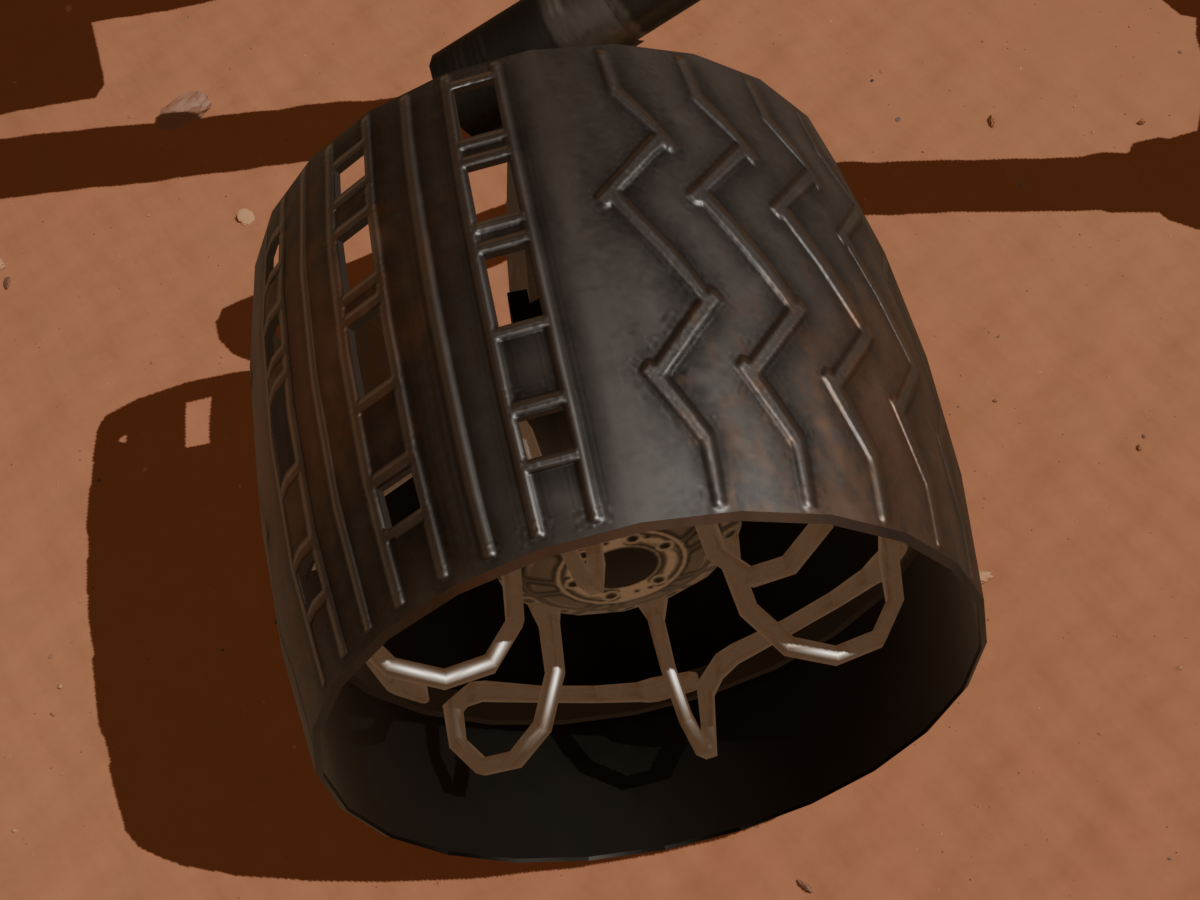
\includegraphics[width=\linewidth]{Images/dr_lighting_clear.png}
        \par\smallskip
        {\small (a) Clear preset}
    \end{minipage}
    \hfill
    \begin{minipage}[b]{0.48\textwidth}
        \centering
        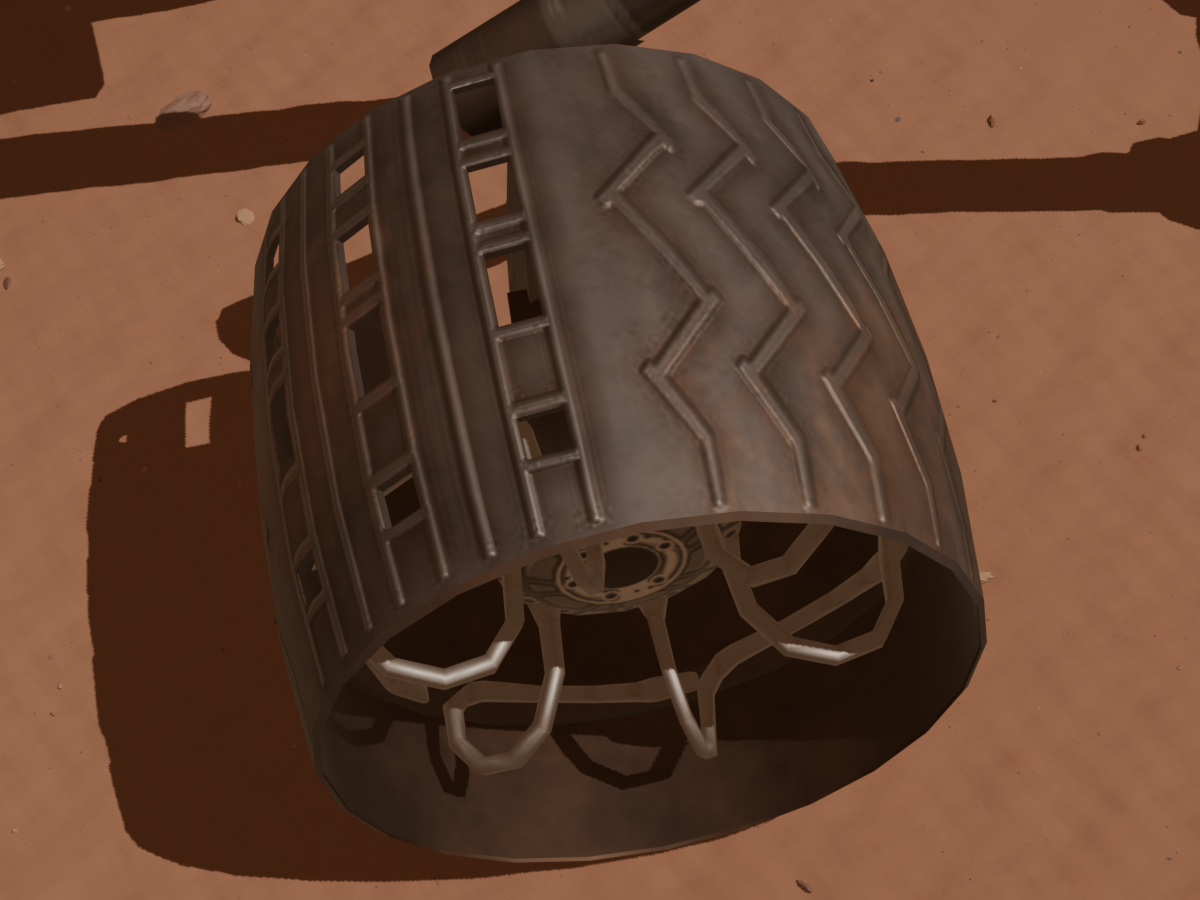
\includegraphics[width=\linewidth]{Images/dr_baseline.png}
        \par\smallskip
        {\small (b) Dusty preset}
    \end{minipage}
    \caption{Clear and dusty rendering presets applied to the same
        normal wheel, with identical camera pose and wheel orientation.
        The dusty preset also changes deposited dust and camera response,
        so the comparison does not isolate illumination alone.}
    \label{fig:dr-lighting}
\end{figure}

\paragraph{Normal surface variation.}
Three surface conditions were considered: no wear, light
wear, and evident wear, as shown in Figure~\ref{fig:dr-surface}. Additional scratches
changed the surface appearance without creating holes or altering the
wheel silhouette. Surface wear did not determine the anomaly label:
a sample was anomalous only when a hole was introduced, and scratches
were excluded from the anomaly mask. Including these patterns among
normal appearances was intended to discourage false alarms caused by
high-contrast marks or local texture changes, simulating real operational wear.

\begin{figure}[htbp]
    \centering
    \begin{minipage}[b]{0.32\textwidth}
        \centering
        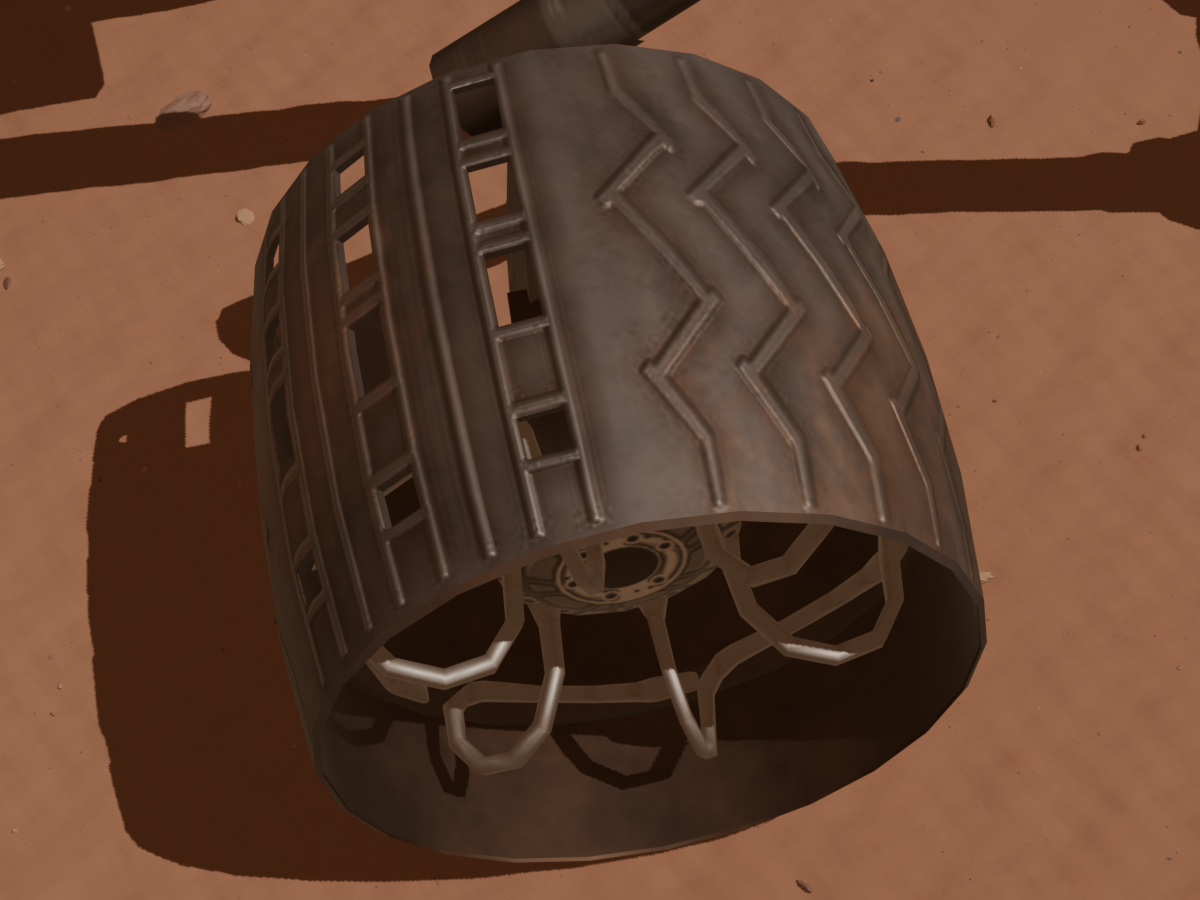
\includegraphics[width=\linewidth]{Images/dr_baseline.png}
        \par\smallskip
        {\small (a) No additional wear}
    \end{minipage}
    \hfill
    \begin{minipage}[b]{0.32\textwidth}
        \centering
        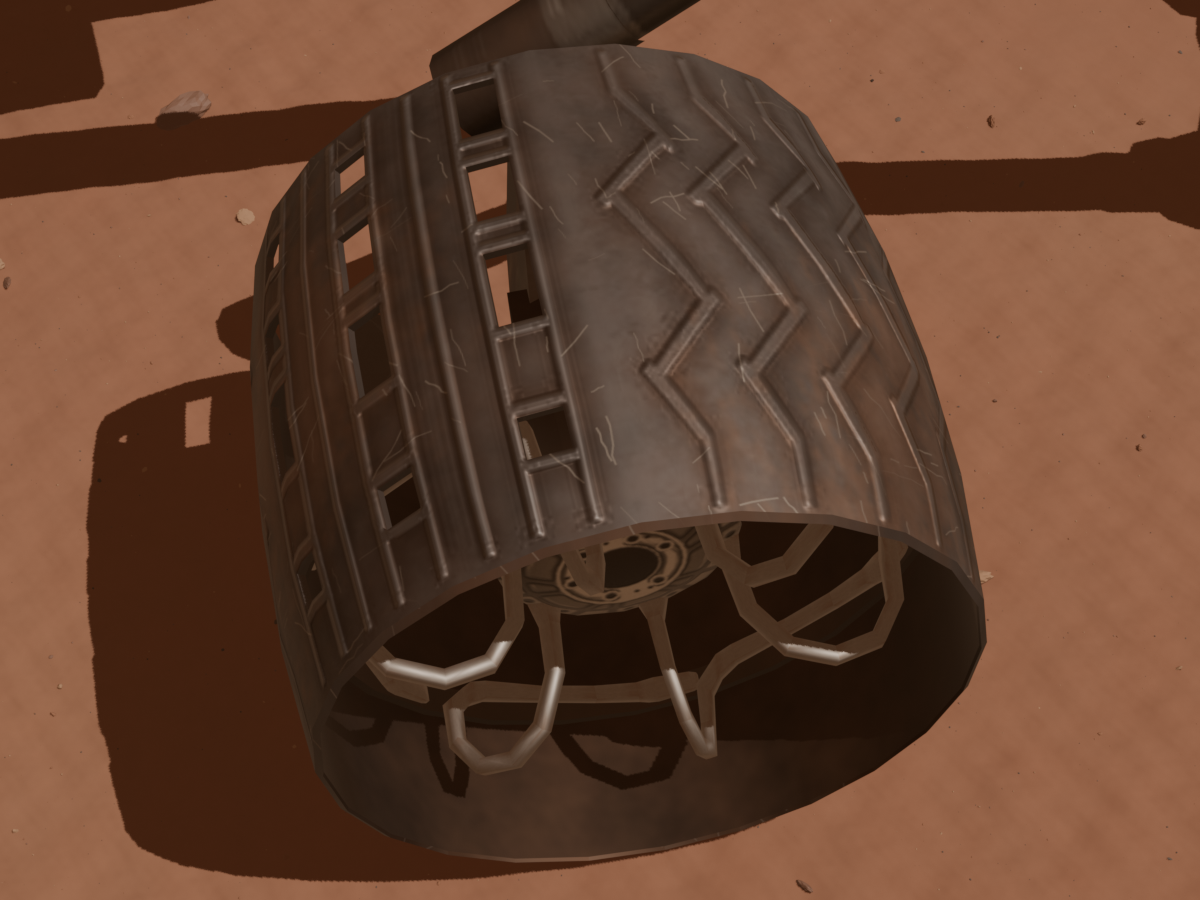
\includegraphics[width=\linewidth]{Images/dr_wear_light.png}
        \par\smallskip
        {\small (b) Light wear}
    \end{minipage}
    \hfill
    \begin{minipage}[b]{0.32\textwidth}
        \centering
        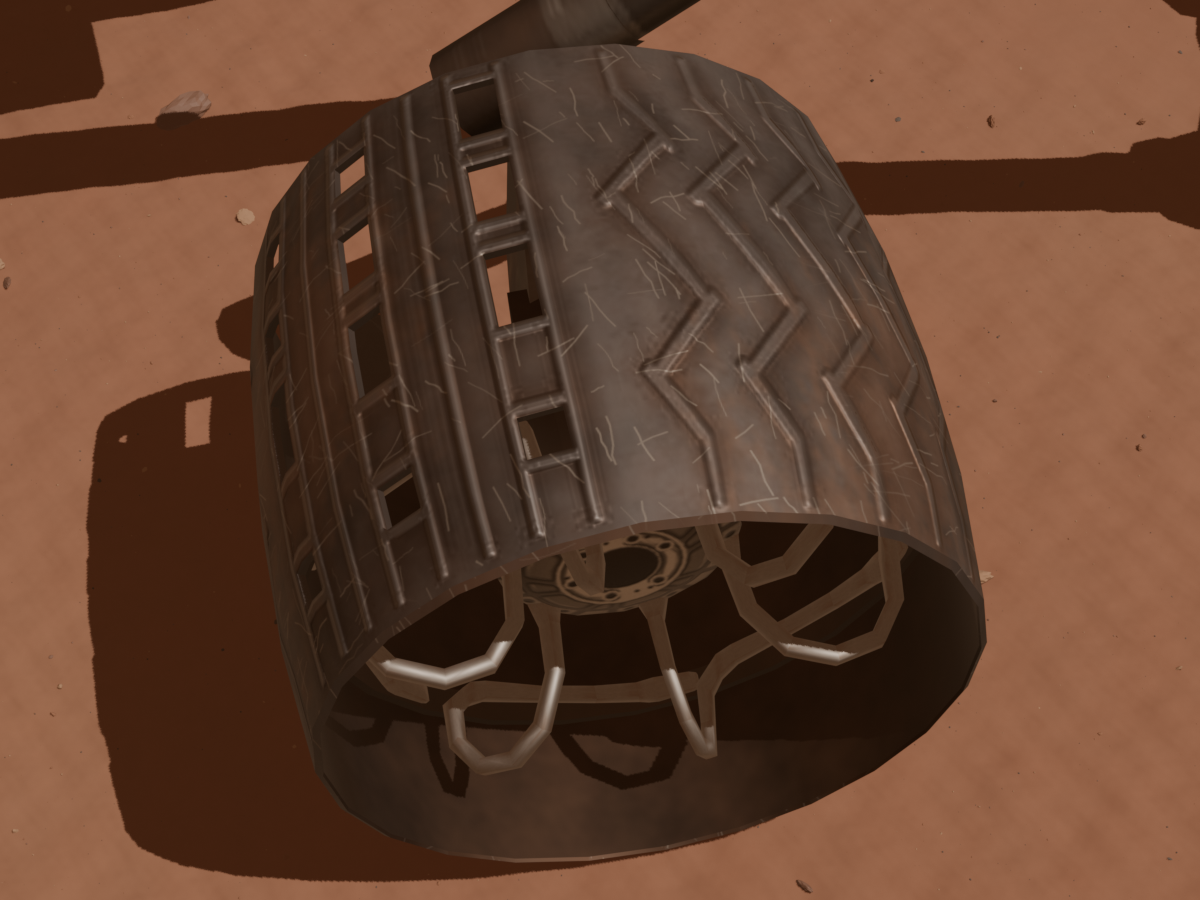
\includegraphics[width=\linewidth]{Images/dr_wear_evident.png}
        \par\smallskip
        {\small (c) Evident wear}
    \end{minipage}
    \caption{Normal surface conditions under identical lighting,
        camera pose, and wheel orientation. All three examples contain
        no injected hole and belong to the normal class.}
    \label{fig:dr-surface}
\end{figure}

\paragraph{Wheel selection and rotation.}
The target wheel was varied across all six rover wheels, introducing
different surrounding suspension and chassis structures. For standalone
normal samples, a shared rotation was applied to all six wheels using
eight phases separated by \(45^\circ\). Rotation changes the visible
arrangement of tread features and surface marks, reducing dependence
on a fixed angular configuration. For damaged samples, wheel orientation
was constrained by the visibility requirements described in
Section~\ref{sec:synthetic-damage-generation}.

\paragraph{Procedural ground detail.}
The local terrain incorporated procedurally generated relief, grains,
rock fragments, and fine surface texture. These features introduce
background clutter and cast shadows near the wheel, which must be
distinguished from the target damage. The generated terrain realization
was kept throughout dataset rendering rather than regenerated for
each sample, for efficiency purposes. Its projected appearance nevertheless varied with camera pose and illumination.

\paragraph{Camera poses.}
Four wheel-centric camera configurations were used:
an overhead view (A), leading and trailing three-quarter views
(C1 and C2), and an upper detail view (D), as shown in
Figure~\ref{fig:dr-camera}. The first three configurations included
the complete wheel, whereas D intentionally captured a closer,
partial view. Small perturbations in camera position, viewing
direction, and focal length provided variation within each configuration.
Changing viewpoint modifies perspective, the visible wheel surface,
and the apparent size of a hole. Whole-wheel views retain more context
but represent small defects with fewer pixels, while the detail view magnifies local features. The different camera configurations were also included to compare detection and localization performance across viewpoints and identify the pose best suited to wheel-damage inspection.

\begin{figure}[ht!]
    \centering
    \begin{minipage}[b]{0.48\textwidth}
        \centering
        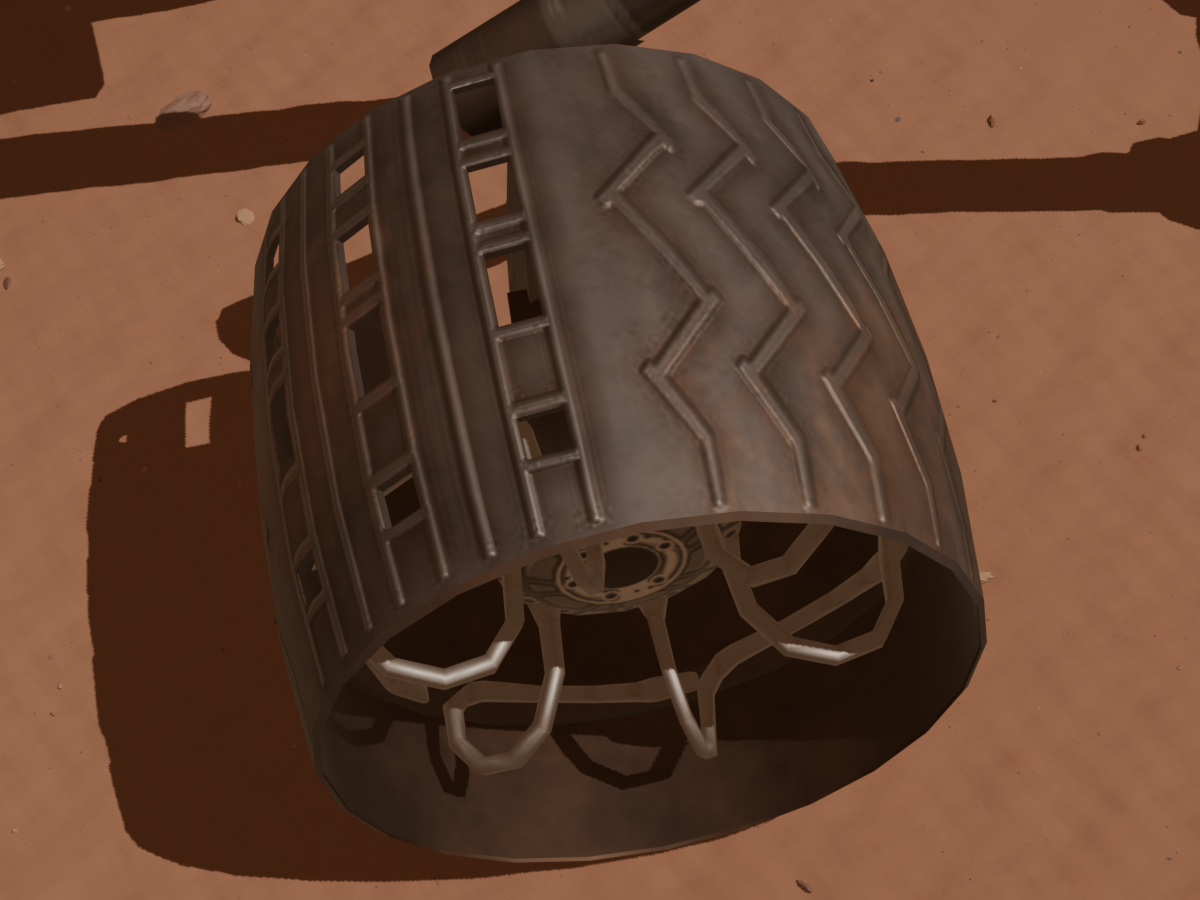
\includegraphics[width=\linewidth]{Images/dr_baseline.png}
        \par\smallskip
        {\small (a) A -- Overhead}
    \end{minipage}
    \hfill
    \begin{minipage}[b]{0.48\textwidth}
        \centering
        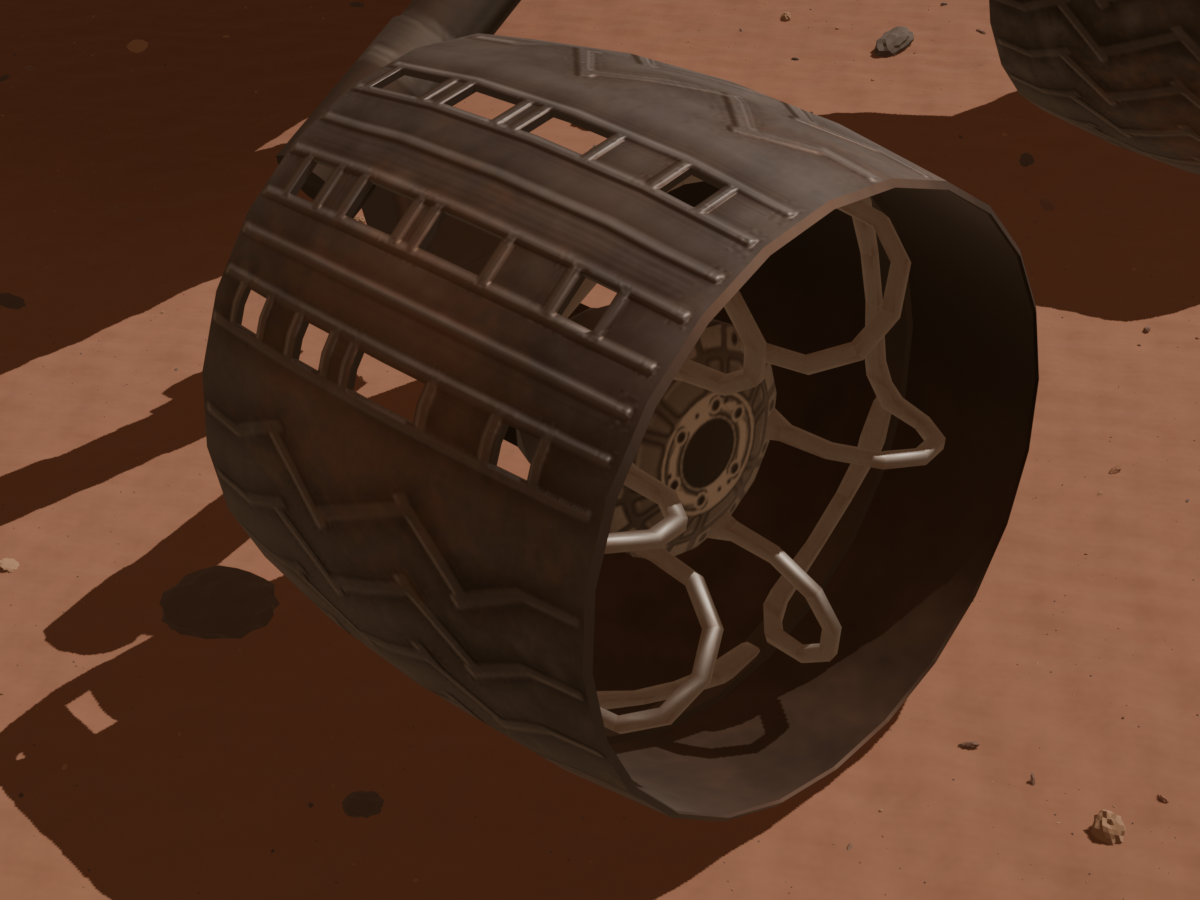
\includegraphics[width=\linewidth]{Images/dr_pose_leading.png}
        \par\smallskip
        {\small (b) C1 -- Leading three-quarter}
    \end{minipage}

    \par\medskip

    \begin{minipage}[b]{0.48\textwidth}
        \centering
        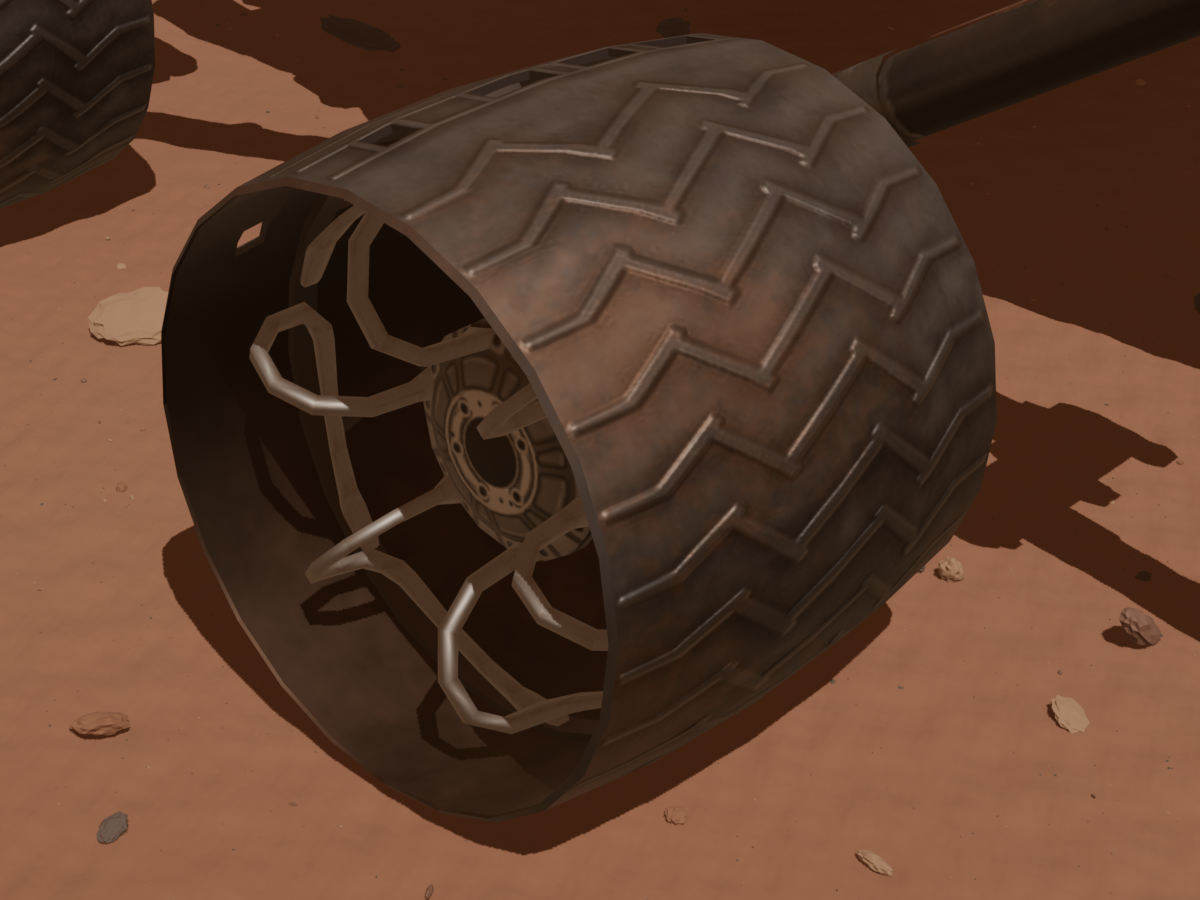
\includegraphics[width=\linewidth]{Images/dr_pose_trailing.png}
        \par\smallskip
        {\small (c) C2 -- Trailing three-quarter}
    \end{minipage}
    \hfill
    \begin{minipage}[b]{0.48\textwidth}
        \centering
        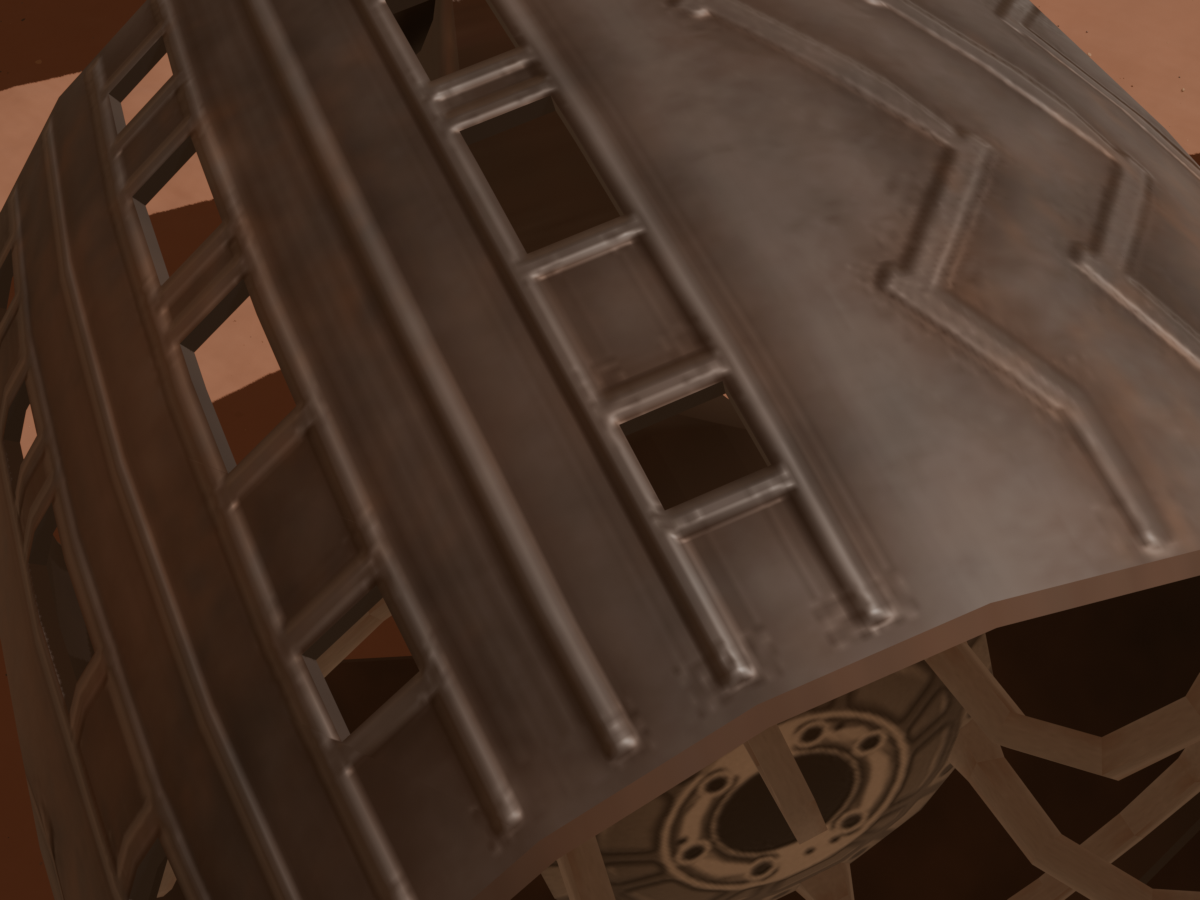
\includegraphics[width=\linewidth]{Images/dr_pose_detail.png}
        \par\smallskip
        {\small (d) D -- Upper detail}
    \end{minipage}
    \caption{The four camera configurations shown for the same
        normal wheel under the dusty preset, without additional wear.
        Wheel orientation is unchanged across views.}
    \label{fig:dr-camera}
\end{figure}

Within each clean/hole pair, lighting, surface wear, camera settings,
and wheel orientation were kept identical. Only the injected hole
distinguished the two scene states, avoiding appearance differences
that could otherwise provide unintended label cues within a pair.

\section{Quality Assurance}
\label{sec:synthetic-quality-assurance}

Quality assurance combined automated checks with visual inspection of selected renders. Geometric and annotation constraints determined sample acceptance, while contrast diagnostics identified potentially challenging examples without automatically excluding them.
The target wheel was checked for appropriate framing and unwanted occlusions. Full-wheel views required the wheel to remain within the image, whereas the partial framing of pose D was intentional and therefore admissible. For anomalous samples, the opening and its complete boundary had to remain visible. Additional checks verified wheel-ground contact and ensured that the ground region covered by the camera remained inside the detailed terrain patch, avoiding exposed patch boundaries or unsupported wheel placement.

Damage masks were required to be spatially consistent with the target-wheel region, and free of random connected components, while severity-dependent thresholds prevented annotations from becoming excessively small. Matched normal and anomalous images were compared to assess the appearance change produced by the anomalous detail and low contrast cases were kept and flagged, provided that the remaining acceptance checks were satisfied.

\section{Final Dataset Composition}
\label{sec:final-synthetic-dataset}

The final dataset contains 10,000 RGB images, comprising 7,500 normal samples and 1,250 matched normal-anomalous pairs. This results in 8,750 normal images and 1,250 anomalous images, each containing one injected hole. Every image is associated with a target-wheel mask, while anomalous images additionally include a binary damage mask.

The training split contains only normal images, allowing the anomaly-detection models to learn wheel appearance without exposure to injected defects. Validation and test splits include both conditions, as summarized in Table~\ref{tab:synthetic-dataset-splits}. Validation contains 500 standalone normal images and 250 pairs, whereas the test split consists of 1,000 pairs. Split assignments were established before rendering, and each pair was treated as an indivisible unit, meaning that an anomalous image and its normal counterpart could not be assigned to different subsets.

\begin{table}[ht!]
    \centering
    \begin{tabular}{@{}l c c c@{}}
        \toprule
        \textbf{Split} & \textbf{Normal} & \textbf{Anomalous} & \textbf{Total} \\
        \midrule
        \midrule
        Training       & 7,000           & 0                  & 7,000          \\
        Validation     & 750             & 250                & 1,000          \\
        Test           & 1,000           & 1,000              & 2,000          \\
        \midrule
        Total          & 8,750           & 1,250              & 10,000         \\
        \bottomrule
    \end{tabular}
    \vspace{5mm}
    \caption{Composition of the synthetic dataset across training, validation, and test splits.}
    \label{tab:synthetic-dataset-splits}
\end{table}

The main category distributions are reported in Table~\ref{tab:synthetic-category-distributions}. The six rover wheels are represented approximately uniformly, with 1,666--1,667 images per wheel. Defect severity and placement distributions refer only to anomalous images, with large defects restricted to the tread.

\begin{table}[ht!]
    \centering
    \begin{tabular}{@{}l l c@{}}
        \toprule
        \textbf{Factor} & \textbf{Categories}       & \textbf{Share (\%)}  \\
        \midrule
        \midrule
        Camera pose     & A / C1 / C2 / D           & 40 / 27.5 / 27.5 / 5 \\
        Lighting        & Dusty / clear             & 75 / 25              \\
        Surface wear    & Current / light / evident & 20 / 45 / 35         \\
        Defect severity & Small / medium / large    & 50 / 40 / 10         \\
        Defect location & Tread / outer shoulder    & 80 / 20              \\
        \bottomrule
    \end{tabular}
    \vspace{5mm}
    \caption{Main category distributions in the final dataset. Camera pose, lighting, and surface wear percentages refer to all 10,000 images; defect severity and location percentages refer to the 1,250 anomalous images.}
    \label{tab:synthetic-category-distributions}
\end{table}

Images were generated through an automated batch pipeline in Blender 5.2 using Eevee, at a resolution of \(1200 \times 900\) pixels with 64 rendering samples, and saved as 8-bit RGB PNG files. For each sample, the prepared scene was restored to its reference state before applying the parameters specified by the generation plan. Standalone normal samples required one render, whereas paired samples required a normal and an anomalous render with matching camera, illumination, surface appearance, and wheel configuration. Annotation information was obtained alongside the RGB renders, and the normal wheel mask was kept for both members of each pair, for possible future use.

\chapter{Synthetic Data-Driven Damage Inspection}

\section{Task Definition}
\label{sec:damage-task-definition}

The second branch of the proposed framework addresses visual wheel inspection through the detection and localization of damage in RGB images. The experiments use the synthetic Curiosity wheel dataset introduced in the previous chapter, with localized holes as the target anomaly class. The objective is both to distinguish normal from damaged observations and to identify the image regions associated with the damage. Accordingly, the methods produce an image anomaly score and a spatial anomaly map, allowing detection and localization to be examined separately.

The problem was approached through visual anomaly detection using a normal-only training setting, consistent with the setting adopted by benchmarks such as MVTec AD \cite{bergmann2019mvtec}. Only normal images from the generated dataset were used for training, while the rendered damaged images and their annotations were reserved for validation and testing. This choice was motivated by the aim of reducing dependence on annotated damage examples during training, rather than fitting a supervised segmentation model directly to the available hole masks. Normality was defined by the absence of the modeled perforations, not by a clear wheel surface, so that other appearance variations remained part of the normal distribution.

Several deep learning-based anomaly detection approaches were investigated to compare their ability to identify localized defects without confusing them with the appearance changes introduced during dataset generation. Compact configurations were also considered in view of the longer-term possibility of onboard inspection. The resulting study provides a controlled assessment of damage detection and localization within the synthetic domain, while validation on real rover imagery remains outside the scope of the present experiments.

\section{Preprocessing}
\label{sec:damage-preprocessing}

All images were loaded as three-channel RGB observations and converted to floating-point tensors. Their pixel intensities were rescaled from the original 8-bit representation to the \([0,1]\) interval before any model-specific normalization.
The experiments included full frame inputs and wheel focused configurations using fixed square crops for each camera pose. The crop windows were defined from normal validation observations and applied consistently across dataset splits, before resizing. At inference, the pose identifier determined the crop, without requiring the damage mask. The already detailed framing of pose D did not receive an additional pose specific crop.
Wheel focused framing was motivated by the aim of dedicating more of the available input resolution to the inspected rover part. The intention was to keep useful surface detail at moderate network input sizes, favoring a controlled camera configuration that centers the target wheel. Figure~\ref{fig:wheel-pose-a-crop} illustrates this preparation for pose A. In a future integration of the two framework branches, the \emph{Rover} category predicted by the scene understanding module could help identify vehicle regions and help further wheel-localization steps. This connection was not implemented in the present work, as the segmentation label does not directly identify individual wheels.

\begin{figure}[ht!]
    \centering
    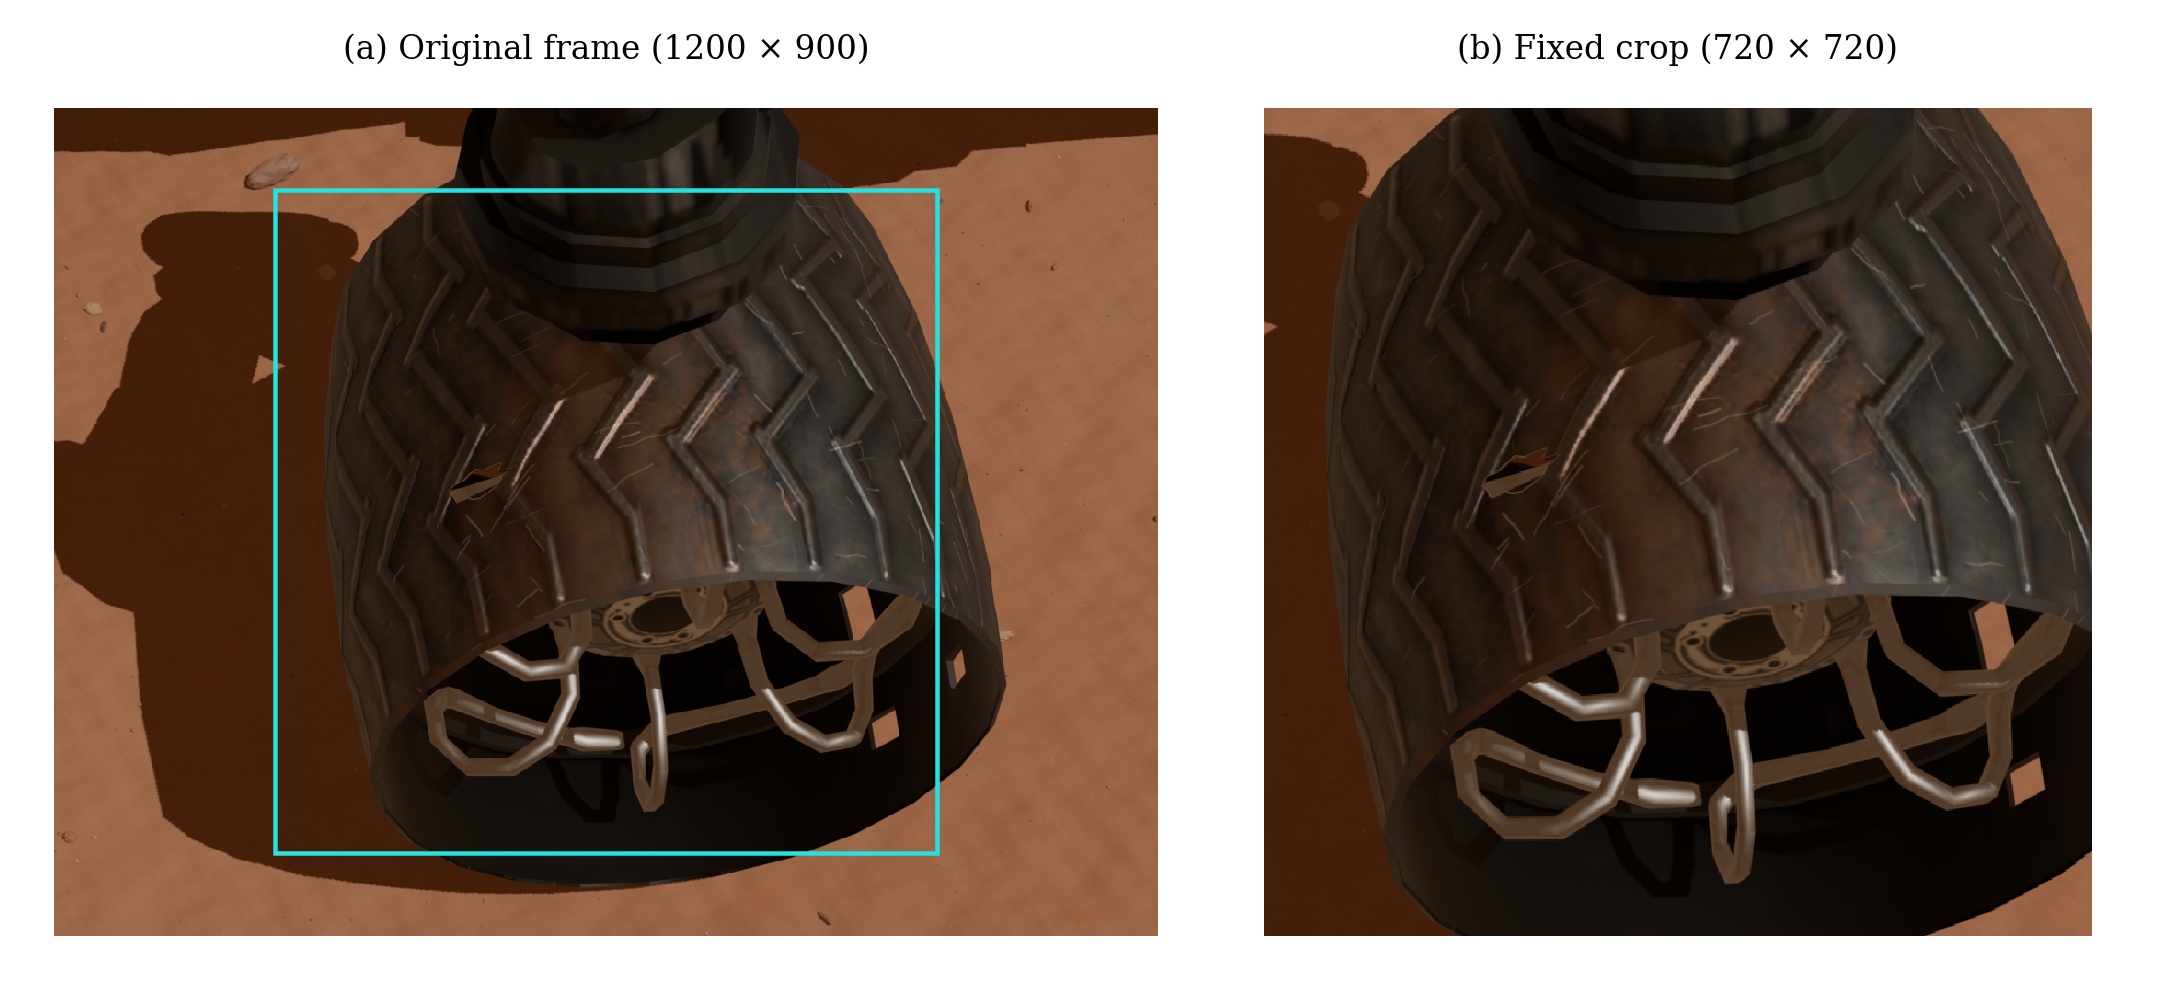
\includegraphics[width=\textwidth]{Images/wheel_pose_a_crop_comparison.png}
    \vspace{3mm}
    \caption{Comparison before and after the fixed crop for camera pose A.
        (a) Original \(1200 \times 900\)-pixel observation, with the crop window
        highlighted in cyan. (b) The retained \(720 \times 720\)-pixel region,
        shown before resizing to the network input resolution.
        Both panels depict the same dataset image.}
    \label{fig:wheel-pose-a-crop}
\end{figure}

Input resolution depended on the model and experimental configuration. It was treated as a compromise between computational cost and the spatial detail available for inspection, because strong downsampling can leave small defects represented by very few pixels, while larger inputs increase processing and memory requirements. The effects of these choices are examined in the evaluation chapter.

\section{Anomaly Detection Models}

The model set was selected with two complementary objectives: comparing different anomaly detection strategies compatible with the normal-only training strategy and investigating their computational requirements for potential onboard inspection. The resulting pool comprises four model families: PatchCore~\cite{roth2022patchcore}, EfficientAD-S (EAD-S)~\cite{batzner2024efficientad}, SuperSimpleNet (SSN)~\cite{rolih2026nolabel}, and TinyGLASS~\cite{bonazzi2026tinyglass}. These methods cover three main principles: matching against stored normal features, measuring student-teacher discrepancies, and learning to discriminate normal observations from synthetic perturbations. In the latter case, anomalous training examples are created from clean inputs in feature or image space, maintaining the separation from the damaged renders reserved for validation and testing.

The selection also contrasts the storage and search costs of a descriptor memory with the feature-extraction and prediction costs of feed-forward networks. PatchCore provides a memory-based reference, whereas the other three models compute anomaly scores through learned network outputs. EAD-S and the ResNet-18 configuration of TinyGLASS represent compact alternatives, while SSN uses a larger Wide ResNet-50-2 feature extractor. This diversity makes it possible to examine the trade-off between damage detection and localization quality, memory requirements, and inference latency, and to assess whether more costly representations help distinguish localized perforations from normal appearance variations.

\subsection{PatchCore}
\label{subsec:patchcore}

PatchCore detects anomalies by comparing local image features with a memory of defect-free examples, rather than learning predefined damage categories~\cite{roth2022patchcore}. A convolutional backbone pretrained on ImageNet remains frozen, with features from two intermediate stages aggregated over local neighborhoods and combined across scales, preserving local detail while incorporating spatial context.

During training, patch descriptors extracted from normal images are collected into a memory bank, from which greedy \emph{coreset} selection retains a representative subset to limit redundancy and reduce the cost of nearest-neighbor searches. At inference, each test patch is compared with the stored descriptors and assigned an anomaly score equal to its Euclidean distance from the nearest neighbor, with the resulting scores mapped back to their spatial positions to form an anomaly map. The image score is based on the most anomalous patch, although the original formulation also applies neighborhood-based reweighting when computing this score~\cite{roth2022patchcore}. Figure~\ref{fig:patchcore_architecture} illustrates this process, from memory construction to patch and image anomaly scoring.

\begin{figure}[htbp]
    \centering
    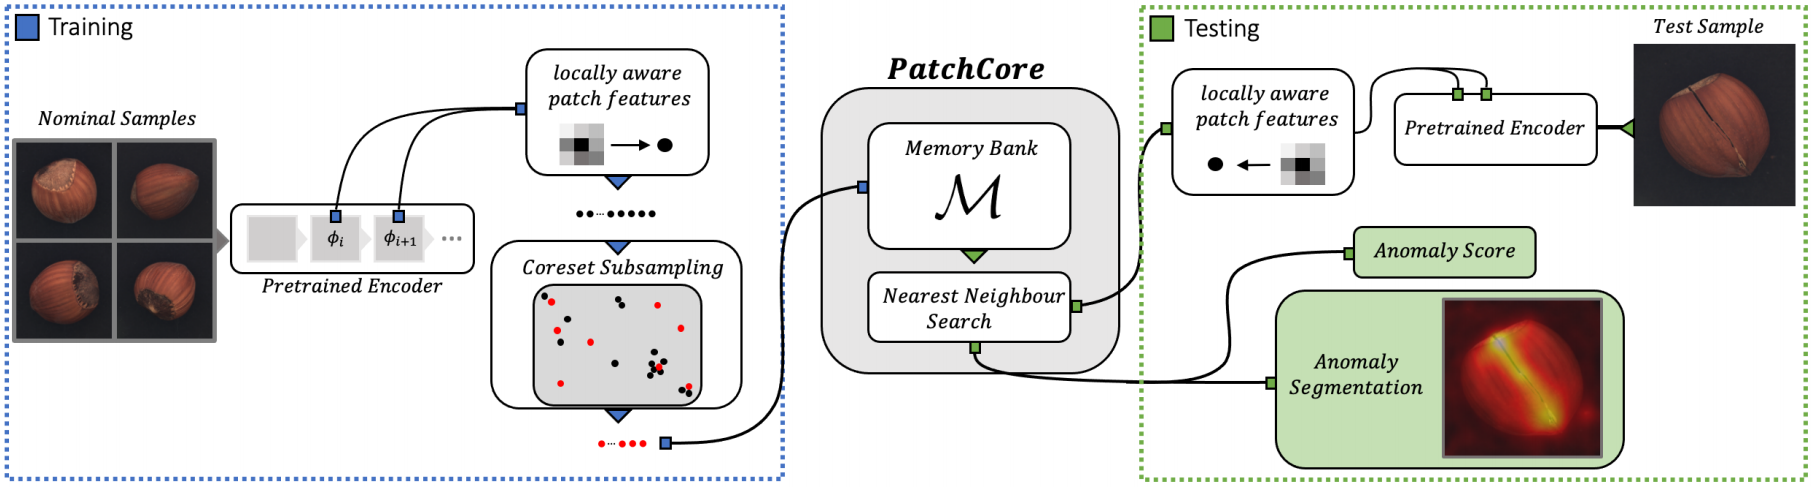
\includegraphics[width=\linewidth]
    {Images/patchcore_original_architecture.png}
    \caption{Original overview of PatchCore: normal-feature memory
        construction on the left and nearest-neighbor-based anomaly
        detection and localization on the right.
        Reproduced from Roth et al.~\cite{roth2022patchcore}.}
    \label{fig:patchcore_architecture}
\end{figure}

PatchCore was included as a memory-based baseline compatible with normal-only training. Its local scoring mechanism is relevant to wheel perforations, which affect limited image regions, while providing both detection and localization outputs. Related applications include BladeSynth, where PatchCore was fitted using normal rendered aero-engine blade images~\cite{eltoum2025bladesynth}, and surface inspection of shock absorber connecting rods, where both the original method and an enhanced variant were evaluated~\cite{zhou2026shockabsorber}. These studies provide precedents for metallic component inspection, without establishing performance on Martian rover imagery.

In this project, a ResNet-18 configuration, denoted PatchCore Small (PC-S), was considered to reduce feature-extraction cost, alongside PatchCore Large (PC-L), which uses Wide ResNet-50-2. Both configurations use frozen pretrained features. To bound memory construction, patches are randomly sampled from each clean image and kept  in a capped candidate reservoir before greedy coreset selection. Consequently, the coreset is selected from bounded candidates rather than from every extracted training patch. This introduces a trade-off between computational cost and coverage of normal appearances. Memory bank size also influences storage requirements and nearest-neighbor inference cost, making it an important factor in the efficiency assessment.

\subsection{EAD-S}
\label{subsec:efficientad}

EfficientAD detects deviations from normal appearance through a student-teacher model, in which a student learns to reproduce a frozen teacher's features using clean images~\cite{batzner2024efficientad}. The teacher is a compact Patch Description Network (PDN), distilled from a deeper pretrained network to avoid executing that larger backbone at inference. Differences between teacher and student outputs provide a local anomaly map, where larger discrepancies indicate possible departures from the normal training distribution.

Because local descriptors may appear normal even when objects are arranged incorrectly, EfficientAD also includes an autoencoder that reconstructs teacher features from the complete image. An additional student output learns the autoencoder's normal reconstruction behavior, allowing the global anomaly map to measure their disagreement while accounting for systematic reconstruction errors. The two maps are calibrated and averaged~\cite{batzner2024efficientad}, as illustrated in Figure~\ref{fig:efficientad_architecture}.

\begin{figure}[htbp]
    \centering
    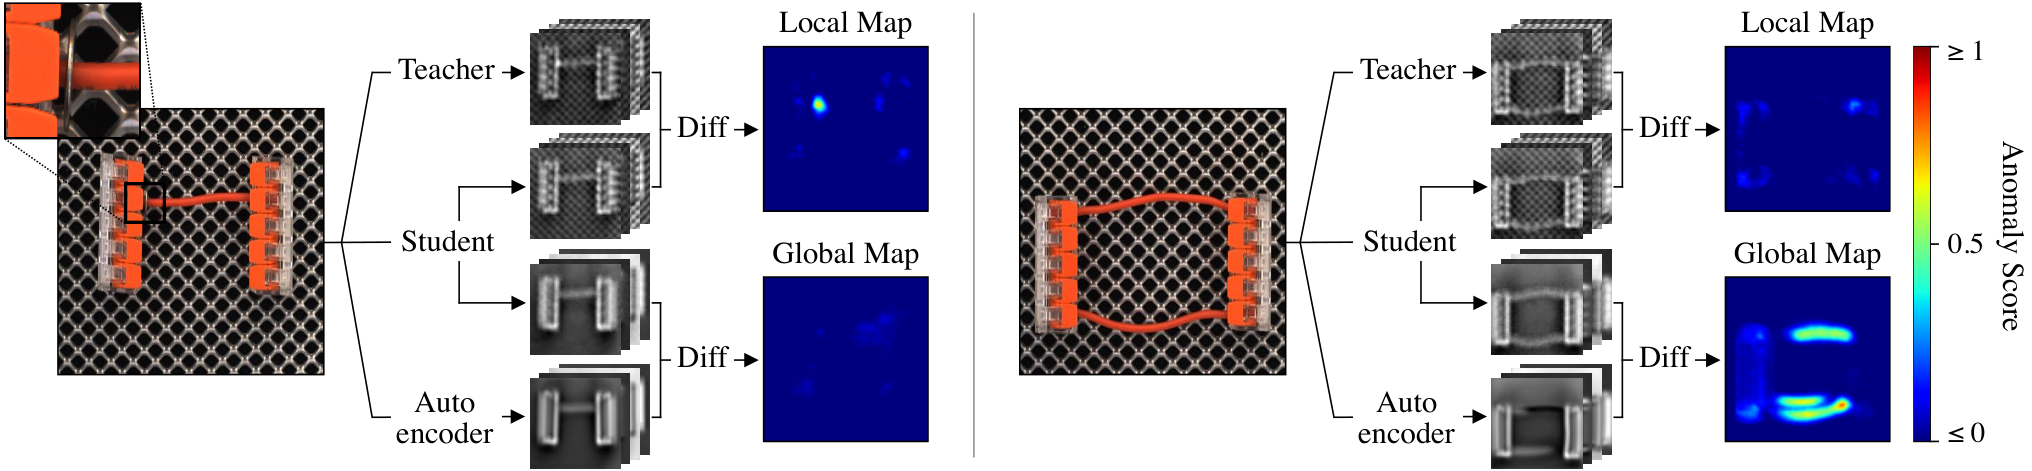
\includegraphics[width=\linewidth]
    {Images/efficientad_original_figure5.png}
    \caption{EfficientAD illustrated on a structural anomaly
        (left) and a logical anomaly (right), showing the local
        and global detection branches.
        Reproduced from Batzner et al.~\cite{batzner2024efficientad}.}
    \label{fig:efficientad_architecture}
\end{figure}

EfficientAD was included to investigate an alternative to PatchCore's memory-based matching, since its inference relies on learned network outputs rather than a nearest-neighbor search over stored descriptors. A related application is automotive inspection on AutoVI, where the authors evaluated EfficientAD alongside other detectors on assembly-line images with variable illumination and cluttered backgrounds~\cite{villanueva2026autovi}. Although these experiments concern assembly defects rather than wheel perforations, they provide a relevant precedent for evaluating the method on mechanical components under variable acquisition conditions.

The experiments used EAD-S, keeping a pretrained teacher while optimizing the student and autoencoder on clean wheel images. Training emphasized the largest feature discrepancies through hard-feature mining and included an auxiliary penalty on ImageNet images to discourage imitation beyond normal wheel appearance. In the global baseline configuration, calibration used only clean validation images, and the maximum of the combined anomaly map provided the image score.

\subsection{SSN}
\label{subsec:supersimplenet}

SSN learns to distinguish normal image features from artificially perturbed ones, allowing a discriminative detector to be trained without examples of actual damage~\cite{rolih2025supersimplenet}. Rather than modifying the input images, it adds Gaussian noise to feature regions selected by thresholded Perlin noise, producing spatially coherent perturbations whose locations provide the training labels. Although the method can also exploit annotated defects, this study considers its normal-only setting.

A pretrained convolutional backbone extracts intermediate features, which are aligned to a common spatial resolution and pooled to incorporate neighboring context. A trainable adapter prepares these features for a segmentation head, while a separate classification head combines the predicted anomaly map with image features to estimate an image score. In the extended formulation, the classification branch receives the unadapted features, allowing the two heads to operate on different representations~\cite{rolih2026nolabel}. Figure \ref{fig:supersimplenet_architecture} illustrates this architecture, including the anomaly generation mechanism that is active during training but bypassed at inference.

\begin{figure}[htbp]
    \centering
    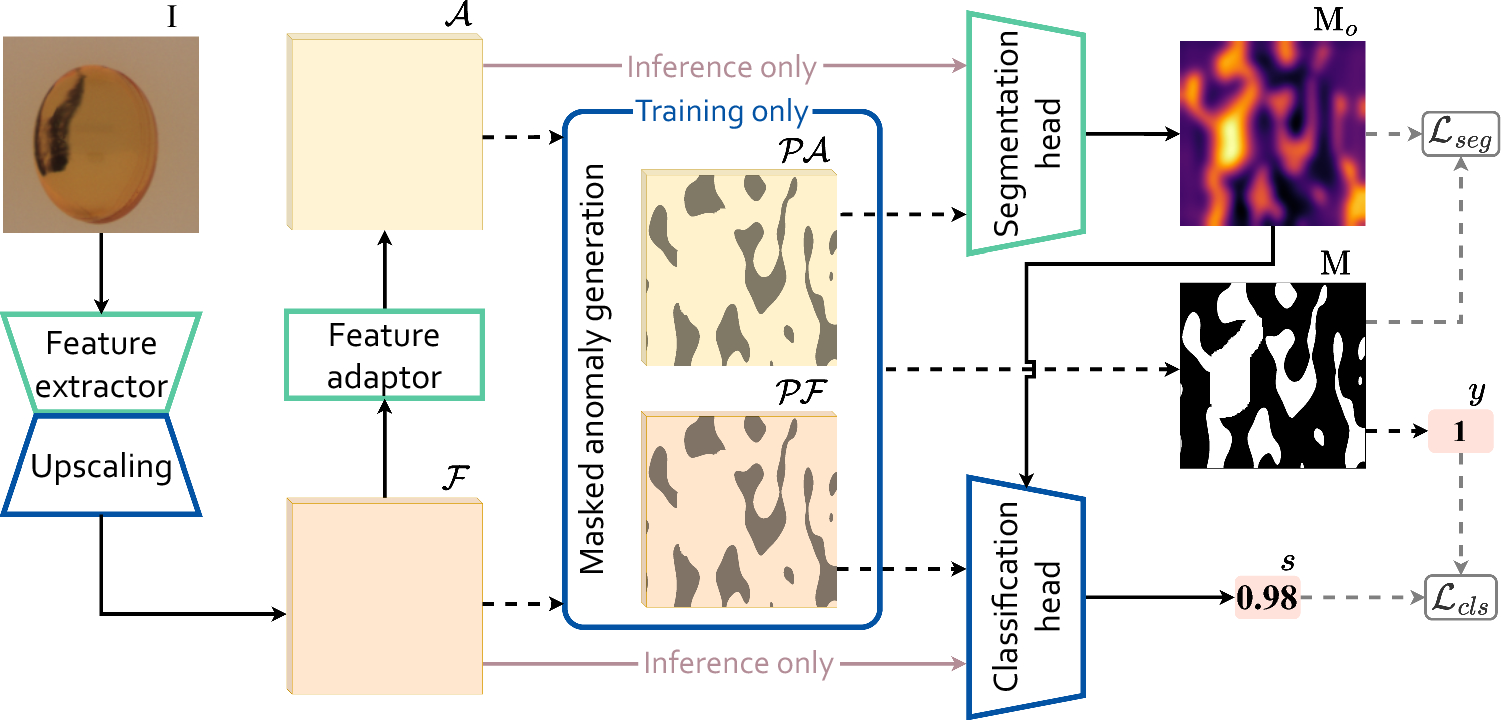
\includegraphics[width=\linewidth]{Images/supersimplenet_original_architecture.png}
    \caption{Architecture of the extended SSN formulation.
        Synthetic feature perturbations are introduced during training,
        whereas inference directly produces an anomaly map and a
        classification score. Reproduced without modification from
        Rolih et al.~\cite{rolih2026nolabel}.
    }
    \label{fig:supersimplenet_architecture}
\end{figure}

SSN was included to compare feature-space anomaly synthesis with PatchCore's memory-based matching and EfficientAD's student-teacher formulation. This comparison investigates whether learning from localized feature perturbations can support the detection of wheel perforations without using damaged renders for weight optimization. Its feed-forward inference also avoids searching a stored descriptor bank, although the computational cost of the pretrained backbone remains relevant. A related application is the normal-only inspection of automotive assemblies on AutoVI, where SSN was evaluated alongside other anomaly detectors~\cite{villanueva2026autovi}.

The project implementation uses a frozen Wide ResNet-50-2 pretrained on ImageNet, extracting features from its second and third residual stages while optimizing the adapter and prediction heads on clean wheel images. The generated perturbations are distinct from the holes rendered in Blender and do not require their annotations. Besides the original classification-head score, the experiments considered an image score obtained by averaging the largest \(1\%\) of the raw anomaly-map values on the native feature grid, before resizing and smoothing. Restricting synthetic perturbations to the target-wheel region was also investigated as an ablation, using the wheel mask during training only.

\subsection{TinyGLASS}
\label{subsec:tinyglass}

TinyGLASS is a compact adaptation of GLASS that learns to separate normal features from synthetic anomalies, replacing the original Wide ResNet backbone with ResNet-18 to reduce feature-extraction cost~\cite{bonazzi2026tinyglass}. Intermediate features are combined across scales and processed by a patch-wise discriminator, which assigns higher scores to regions that depart from the normal training distribution.

Training combines the two complementary synthesis strategies introduced by GLASS. Local Anomaly Synthesis (LAS) creates altered image regions by blending external textures within randomized masks, whereas Global Anomaly Synthesis (GAS) perturbs normal features with Gaussian noise and refines them through gradient ascent. These gradient-guided perturbations provide difficult negative examples, while projection constraints limit their distance from normal features~\cite{chen2025glass}. Combining image alterations with feature perturbations exposes the discriminator to both visible appearance changes and deviations close to normality. The synthesis mechanisms are used only during training, leaving a feed-forward prediction path at inference, as illustrated in Figure~\ref{fig:tinyglass_architecture}.

\begin{figure}[htbp]
    \centering
    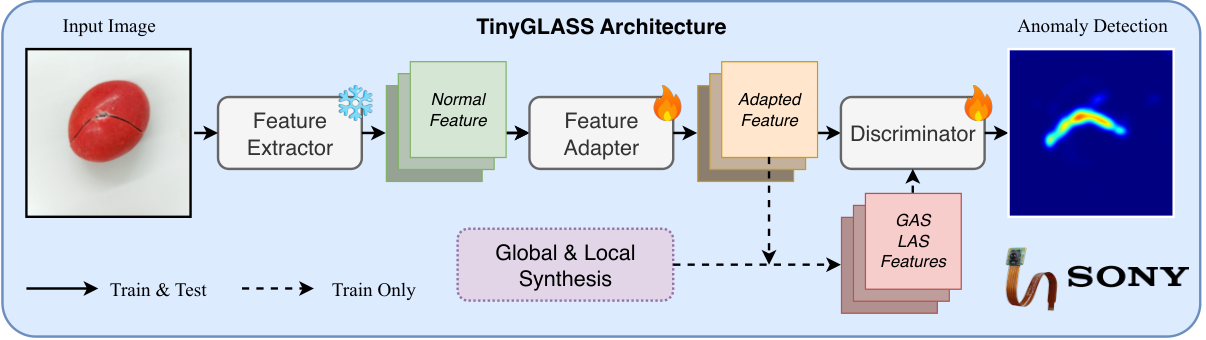
\includegraphics[width=\linewidth]
    {Images/tinyglass_original_architecture.png}
    \caption{Original TinyGLASS architecture, showing the
        feature-processing path and the anomaly synthesis
        mechanisms used during training only.
        Reproduced without modification from
        Bonazzi et al.~\cite{bonazzi2026tinyglass},
        under the
        \href{https://creativecommons.org/licenses/by/4.0/}
        {CC BY 4.0 license}.}
    \label{fig:tinyglass_architecture}
\end{figure}

TinyGLASS was selected to examine the accuracy-efficiency trade-off of a compact synthesis-based detector. In the original study, the method was evaluated on the custom M\&Ms candy dataset (MMS), including a crack-hole category, and deployed on the Sony IMX500 sensor~\cite{bonazzi2026tinyglass}, providing a related example of localized defect inspection.

The baseline implementation kept the ImageNet-pretrained ResNet-18 frozen and used fixed patch pooling for feature compression, without the separate trainable adapter shown in the original figure. Alongside texture-based LAS, a task-specific variant generated irregular, darkened regions inside the target wheel to approximate the appearance of perforations. These two-dimensional alterations were created from clean renders and their wheel masks, rather than from the damaged Blender images, and required no masks during inference. Feature resolution was also varied to examine the balance between computational cost and localization detail. The predicted anomaly maps were resized and smoothed, whereas the image score was obtained from the maximum patch score before this postprocessing.

The TinyGLASS configurations with \(384\times384\) and \(512\times512\) inputs are denoted TG-384 and TG-512, respectively.

\section{Evaluation Metrics}
\label{sec:damage-evaluation-metrics}

Performance is evaluated at two levels: image-level detection, which distinguishes clean images from images containing anomalous wheel damage, and pixel-level localization, which compares the anomaly maps with the ground truth hole masks. Both levels are assessed using the area under the receiver operating characteristic curve (AUROC) and Average Precision (AP), without selecting a fixed decision threshold.

These metrics are defined as
\begin{equation}
    \begin{aligned}
        \mathrm{AUROC}
         & = \int_0^1 \mathrm{TPR}(u)\,\mathrm{d}u, \\
        \mathrm{AP}
         & = \sum_j (R_j - R_{j-1})P_j,
    \end{aligned}
    \label{eq:damage-evaluation-metrics}
\end{equation}
where \(\mathrm{TPR}(u)\) is the True Positive Rate at False Positive Rate (FPR) \(u\), while \(P_j\) and \(R_j\) denote precision and recall at successive decreasing score thresholds, with \(R_0=0\). Scores and labels are accumulated over the entire evaluated partition rather than averaging metrics across individual images.

AUROC describes the ability to rank anomalous images or pixels above normal ones, whereas AP summarizes the precision achieved as recall increases. AP is particularly relevant to localization because defect pixels occupy a small proportion of the input, so even a low false positive rate can produce many incorrect detections when normal pixels dominate \cite{saito2015precisionrecall}. Since AP also depends on anomaly prevalence, comparisons between configurations must account for differences in the evaluated data.

Localization is also examined using Per-Region Overlap (PRO), which measures the fraction of detected pixels within each connected ground truth anomalous region and averages these fractions with equal weight. This prevents larger defects from dominating the evaluation just because of their area \cite{bergmann2021mvtec}. The normalized area under the PRO curve (AUPRO) is reported up to false positive rates of \(0.05\), \(0.10\), and \(0.30\), with the stricter limits emphasizing anomalous detection when fewer false detections are permitted.

%The primary pixel metrics consider the entire processed image. Additional wheel restricted AUROC and AP scores are computed within the target-wheel mask from the corresponding clean render, allowing localization to be assessed without contributions from background pixels. This mask defines an evaluation region and is not required as an input during inference. 
Computational efficiency is assessed separately through inference latency and GPU memory measurements, with the measurement conditions specified in the evaluation chapter.

\chapter{Evaluation of Lightweight Scene Understanding}

\section{Experimental Setup}
\label{sec:segmentation-experimental-setup}

Deployment benchmarks were run on a single NVIDIA T4 GPU in the Kaggle environment. Latency was averaged over 50 forward passes after 10 warm-up runs, with synchronization ensuring that GPU execution had completed before each measurement ended. Energy and peak memory were measured in a separate loop that continued for at least 100 inference runs and 30 seconds. GPU power and memory were sampled every 20~ms through the NVIDIA Management Library (NVML), and energy per image was obtained by dividing the estimated GPU energy consumed during the loop by the number of processed images.

\section{Segmentation Accuracy}
\label{sec:segmentation-accuracy}

The various architectures were evaluated on the S5Mars test split, using the checkpoint with the highest validation mIoU for each training run. The U-Net, DeepLab, and SegFormer-B0 followed the training procedure described in Chapter~2, using 30 epochs for training, whereas the two LCNet variants were trained for 60 epochs, without data augmentation or oversampling. Table~\ref{tab:s5mars-reference-accuracy} reports the results obtained, the validation mIoU used for checkpoint selection alongside the test mIoU and pixel accuracy, keeping model selection separate from the final evaluation.

\begin{table}[ht!]
    \centering
    \small
    \setlength{\tabcolsep}{4pt}
    \begin{tabular}{@{}l c c c@{}}
        \toprule
        \textbf{Configuration}                   &
        \shortstack{\textbf{Val} \textbf{mIoU}}  &
        \shortstack{\textbf{Test} \textbf{mIoU}} & \textbf{Test PA}                 \\
        \midrule
        \midrule
        U-Net (R34)                              & 81.52            & 64.55 & 91.73 \\
        U-Net (MV2)                              & 71.98            & 64.57 & 91.22 \\
        DeepLabV3 (R34)                          & 83.14            & 73.79 & 91.63 \\
        DeepLabV3+ (MV2)                         & 80.81            & 64.07 & 90.59 \\
        SegFormer-B0                             & 80.28            & 75.55 & 91.27 \\
        \midrule
        LCNet\(_{3,7}\)                          & 60.59            & 57.89 & 88.87 \\
        LCNet\(_{3,11}\)                         & 64.54            & 59.11 & 88.98 \\
        \bottomrule
    \end{tabular}
    \vspace{5mm}
    \caption{S5Mars accuracy of the evaluated FP32 configurations. Validation mIoU identifies the selected checkpoint, while test metrics describe its held-out performance.}
    \label{tab:s5mars-reference-accuracy}
\end{table}
SegFormer-B0 achieved the highest test mIoU, 75.55\%, followed by DeepLabV3 with ResNet34 at 73.79\%. Its accuracy is particularly relevant to the lightweight objective: with 3.72 million parameters, compared with 26.01 million for DeepLabV3, SegFormer-B0 obtained a higher mIoU with approximately 86\% fewer parameters (Table~\ref{tab:segmentation-architecture-static-comparison}). U-Net with ResNet34 achieved the highest pixel accuracy, 91.73\%, whereas SegFormer-B0 led on average IoU.

U-Net with MobileNetV2 retained essentially the same test mIoU as its ResNet34 counterpart, 64.57\% versus 64.55\%, while reducing the parameter count by approximately 73\%. The LCNet variants explored a much smaller number of parameters: LCNet\(_{3,7}\) and LCNet\(_{3,11}\) reached 57.89\% and 59.11\% mIoU with only 0.51 and 0.73 million parameters, respectively. Together, these results show the available trade-off between class-averaged accuracy and parameter storage, from the higher accuracy SegFormer-B0 configuration to the sub-million-parameter LCNet models.

The ranking also differs from the aggregate Mars-Bench results, where U-Net was the strongest segmentation baseline under frozen backbone feature extraction~\cite{purohit2025marsbench}. Here, SegFormer-B0 leads the S5Mars comparison after end-to-end fine-tuning, while the MobileNetV2 and LCNet configurations extend the study toward lower parameter budgets. Therefore Mars-Bench provides context for the architectural comparison, even though differences in training procedure prevent a direct ranking across the two studies.

Table~\ref{tab:s5mars-per-class-iou} reports test IoU for the target class categories. The aggregate mIoU corresponds to the mean over these categories, while the additional \emph{Background} identifier is not included in the table, given its absence in the ground truth labels. The definitions and aggregation procedure are given in Section~\ref{sec:segmentation-evaluation-metrics}.

\begin{table}[ht!]
    \centering
    \small
    \setlength{\tabcolsep}{3pt}
    \begin{tabular}{@{}l c c c c c c c c@{}}
        \toprule
        \textbf{Model}                              & \textbf{Bedrock} & \textbf{Hole}  &
        \textbf{Ridge}                              & \textbf{Rock}    & \textbf{Rover} &
        \shortstack{\textbf{Sand /}\\\textbf{Soil}} & \textbf{Sky}     & \textbf{Track}                                                 \\
        \midrule
        \midrule
        U-Net (R34)                                 & 73.32            & 9.75           & 92.28 & 26.47 & 67.99 & 89.95 & 94.56 & 62.07 \\
        U-Net (MV2)                                 & 71.60            & 0.00           & 92.17 & 21.58 & 82.52 & 89.34 & 94.26 & 65.11 \\
        DeepLabV3 (R34)                             & 73.28            & 56.70          & 91.91 & 27.81 & 84.27 & 89.69 & 94.04 & 72.61 \\
        DeepLabV3+ (MV2)                            & 70.55            & 9.65           & 91.89 & 21.97 & 84.99 & 88.39 & 94.50 & 50.59 \\
        SegFormer-B0                                & 71.85            & 78.11          & 90.20 & 21.77 & 83.03 & 89.48 & 94.02 & 75.96 \\
        \midrule
        LCNet\(_{3,7}\)                             & 67.08            & 9.26           & 90.42 & 17.18 & 73.72 & 86.45 & 92.95 & 26.09 \\
        LCNet\(_{3,11}\)                            & 67.42            & 9.49           & 90.77 & 18.85 & 72.48 & 86.60 & 93.62 & 33.63 \\
        \bottomrule
    \end{tabular}
    \vspace{5mm}
    \caption{Per-class IoU on the S5Mars test split. Model abbreviations and selected checkpoints are the same as in Table~\ref{tab:s5mars-reference-accuracy}, with a 60-epoch training budget for the LCNet variants and 30 epochs for the other configurations.}
    \label{tab:s5mars-per-class-iou}
\end{table}
All seven configurations achieved IoUs above 92\% for \emph{Sky}, 90\% for \emph{Ridge}, and 86\% for \emph{Sand/Soil}, including the compact LCNet models. SegFormer-B0 stood out on \emph{Hole} and \emph{Track}, reaching 78.11\% and 75.96\%, whereas DeepLabV3+ with MobileNetV2 produced the highest \emph{Rover} IoU, 84.99\%. The main remaining weakness was \emph{Rock}, for which IoU stayed below 28\% across all configurations.

%\paragraph{Qualitative comparison.}
Figure~\ref{fig:s5mars-model-prediction-comparison} compares the seven models on an S5Mars test image, showing the original scene, its ground truth, and the predicted segmentation masks. The scene contains exposed bedrock, sandy soil, and scattered rocks, with similar colors and textures making the distinction between Rock and Bedrock particularly challenging. Most models reproduce the large division between bedrock and soil, while differences become thinner around individual rocks and local boundaries. The contrast is visible in the lower right area, where SegFormer-B0 and DeepLabV3 ResNet34 are the only models to recognize the isolated rock as Rock, with the latter recovering only part of it. The remaining models classify the object as Bedrock, while the LCNet variants also miss smaller rocks and divide the lower bedrock region into patches separated by soil.

\begin{figure}[ht!]
    \centering
    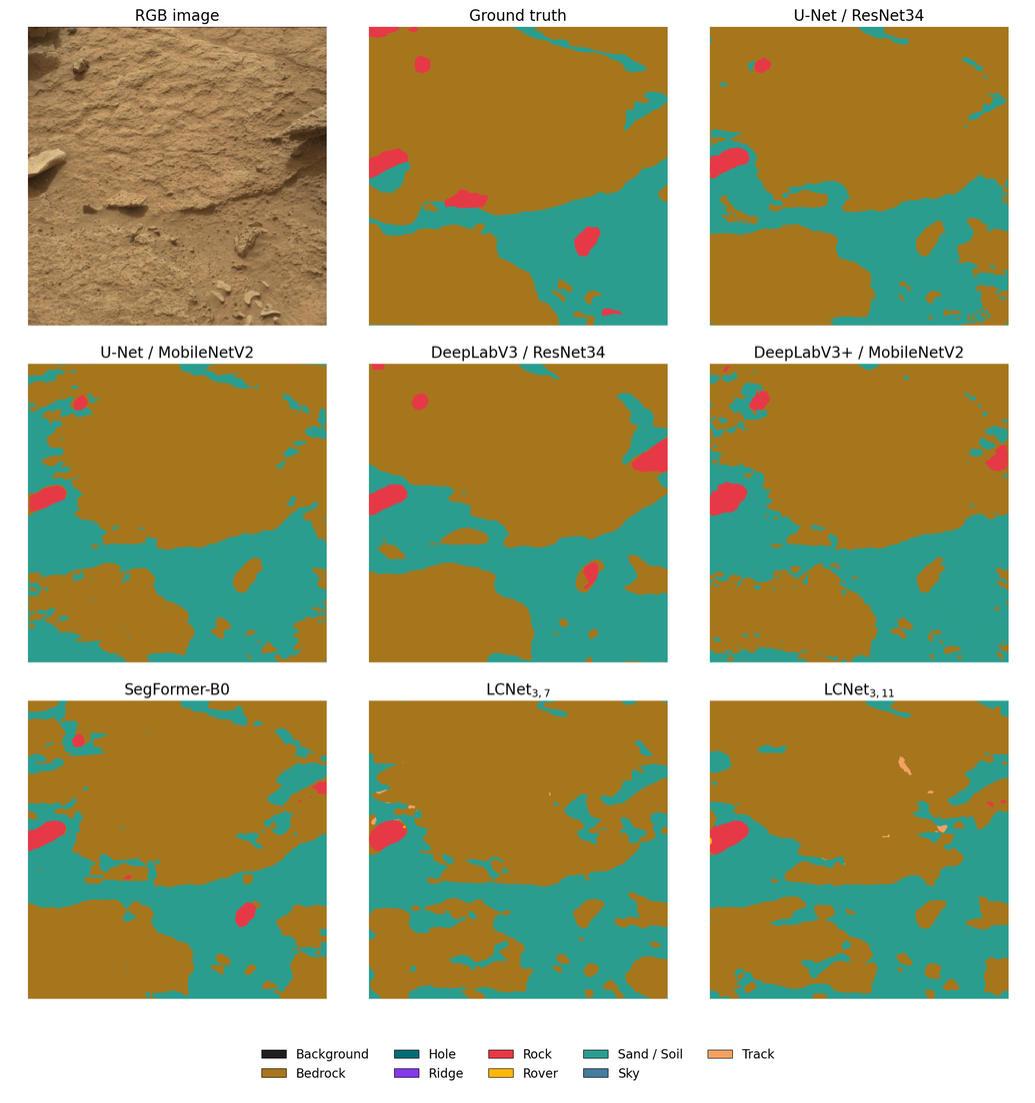
\includegraphics[width=\textwidth]{Images/s5mars_model_prediction_comparison.png}
    \caption{Qualitative comparison on an S5Mars test image, showing the RGB input, ground truth, and predictions of the seven evaluated configurations with a shared class color mapping.}
    \label{fig:s5mars-model-prediction-comparison}
\end{figure}

\section{Quantization Results}
\label{sec:quantization-results}

Table~\ref{tab:s5mars-quantization-accuracy-efficiency} compares the previous results with the PTQ and QAT deployment variants described in Section~\ref{sec:optimization-quantization}. Accuracy was still evaluated on the S5Mars test split, whereas latency, energy per image, and peak GPU memory were measured through separate inference benchmarks with a batch size of one and an input resolution of \(512 \times 512\). LCNet was not included in this quantization campaign, given their already low parameter count and efficiency.

\begin{table}[ht!]
    \centering
    \small
    \setlength{\tabcolsep}{5pt}
    \begin{tabular}{@{}l r r r r r@{}}
        \toprule
        \textbf{Variant}                                    &
        \shortstack{\textbf{Test mIoU}\\\textbf{(\%)}}      &
        \shortstack{\textbf{\(\Delta\)mIoU}\\\textbf{(pp)}} &
        \shortstack{\textbf{Latency}\\\textbf{(ms)}}        &
        \shortstack{\textbf{Energy}\\\textbf{(mJ/image)}}   &
        \shortstack{\textbf{GPU peak}\\\textbf{(MiB)}}                                               \\
        \midrule
        \midrule

        \multicolumn{6}{@{}l}{\textit{U-Net (R34)}}                                             \\
        FP32                                                & 64.55 & --    & 16.30 & 1213.08 & 1128 \\
        FP16                                                & 64.55 & 0.00  & 9.19  & 659.76  & 872  \\
        PTQ INT8                                            & 64.51 & -0.04 & 5.82  & 304.10  & 888  \\
        QAT INT8                                            & 65.24 & +0.69 & 4.81  & 231.42  & 1106 \\
        \midrule

        \multicolumn{6}{@{}l}{\textit{U-Net (MV2)}}                                          \\
        FP32                                                & 64.57 & --    & 11.87 & 878.80  & 1364 \\
        FP16                                                & 64.61 & +0.04 & 8.16  & 523.07  & 1236 \\
        PTQ INT8                                            & 61.55 & -3.02 & 4.17  & 199.96  & 1168 \\
        QAT INT8                                            & 65.00 & +0.42 & 3.57  & 162.66  & 912  \\
        \midrule

        \multicolumn{6}{@{}l}{\textit{DeepLabV3 (R34)}}                                         \\
        FP32                                                & 73.79 & --    & 56.27 & 3977.25 & 414  \\
        FP16                                                & 73.79 & 0.00  & 14.03 & 1016.14 & 284  \\
        PTQ INT8                                            & 73.55 & -0.23 & 7.19  & 455.34  & 856  \\
        QAT INT8                                            & 73.62 & -0.17 & 8.65  & 523.71  & 1130 \\
        \midrule

        \multicolumn{6}{@{}l}{\textit{DeepLabV3+ (MV2)}}                                     \\
        FP32                                                & 64.07 & --    & 8.84  & 653.72  & 706  \\
        FP16                                                & 64.07 & 0.00  & 6.03  & 377.88  & 706  \\
        PTQ INT8                                            & 59.14 & -4.93 & 4.02  & 159.19  & 628  \\
        QAT INT8                                            & 65.63 & +1.57 & 3.01  & 115.34  & 450  \\
        \midrule

        \multicolumn{6}{@{}l}{\textit{SegFormer-B0}}                                                 \\
        FP32                                                & 75.55 & --    & 11.88 & 835.72  & 1550 \\
        FP16                                                & 75.55 & 0.00  & 7.17  & 432.07  & 1294 \\
        PTQ INT8                                            & 75.60 & +0.05 & 5.92  & 327.99  & 1118 \\
        QAT INT8                                            & 76.93 & +1.38 & 5.66  & 291.76  & 1008 \\
        \bottomrule
    \end{tabular}

    \vspace{5mm}
    \caption{
        Accuracy and inference resource measurements for the selected
        configurations. Latency is the mean forward pass time
        with inputs already on the device, excluding preprocessing.
        Peak GPU memory includes the resident model or engine and
        buffers. FP32 and FP16 use ONNX Runtime CUDA, PTQ uses ONNX
        Runtime TensorRT with fallback, and QAT uses TensorRT directly.
        INT8 denotes selective mixed-precision execution, with
        Conv-only quantization for SegFormer-B0.
    }
    \label{tab:s5mars-quantization-accuracy-efficiency}
\end{table}

FP16 conversion left test accuracy essentially unchanged across all five models, with the largest absolute mIoU difference remaining below 0.04\%. Across the five FP16 comparisons, the reported energy reduction ranged from 40.5\% to 74.5\%. PTQ introduced larger, model-dependent accuracy changes. U-Net with ResNet34 lost 0.04\%, SegFormer-B0 gained 0.05\%, and DeepLabV3 with ResNet34 lost 0.23\%. The two MobileNetV2 configurations were more sensitive in these experiments: U-Net lost 3.02\% and DeepLabV3+ lost 4.93\%, despite their lower latency and energy consumption.

The selected QAT configurations exceeded the corresponding FP32 test mIoU for four of the five models. SegFormer-B0 reached 76.93\%, an increase of 1.38\%, while DeepLabV3+ with MobileNetV2 reached 65.63\%, an increase of 1.57\%. DeepLabV3 with ResNet34 remained slightly below its FP32 counterpart, with a decrease of 0.17\%. These results describe the complete QAT optimization procedure, which included supervised fine-tuning and teacher distillation.

Figure~\ref{fig:s5mars-quantization-miou-energy} shows test mIoU versus measured GPU energy per image for the 20 examined configurations. Among these recorded points, QAT DeepLabV3+ and QAT SegFormer-B0 define the observed accuracy-energy frontier: neither has an alternative with both no greater energy consumption and no lower mIoU. DeepLabV3+ required the least measured energy, 115.34~mJ per image, whereas SegFormer-B0 provided the highest test mIoU at 291.76~mJ per image. Their comparison illustrates the remaining choice between a lower inference energy budget and more accurate segmentation, rather than identifying one configuration as preferable for every deployment requirement.

\begin{figure}[ht!]
    \centering
    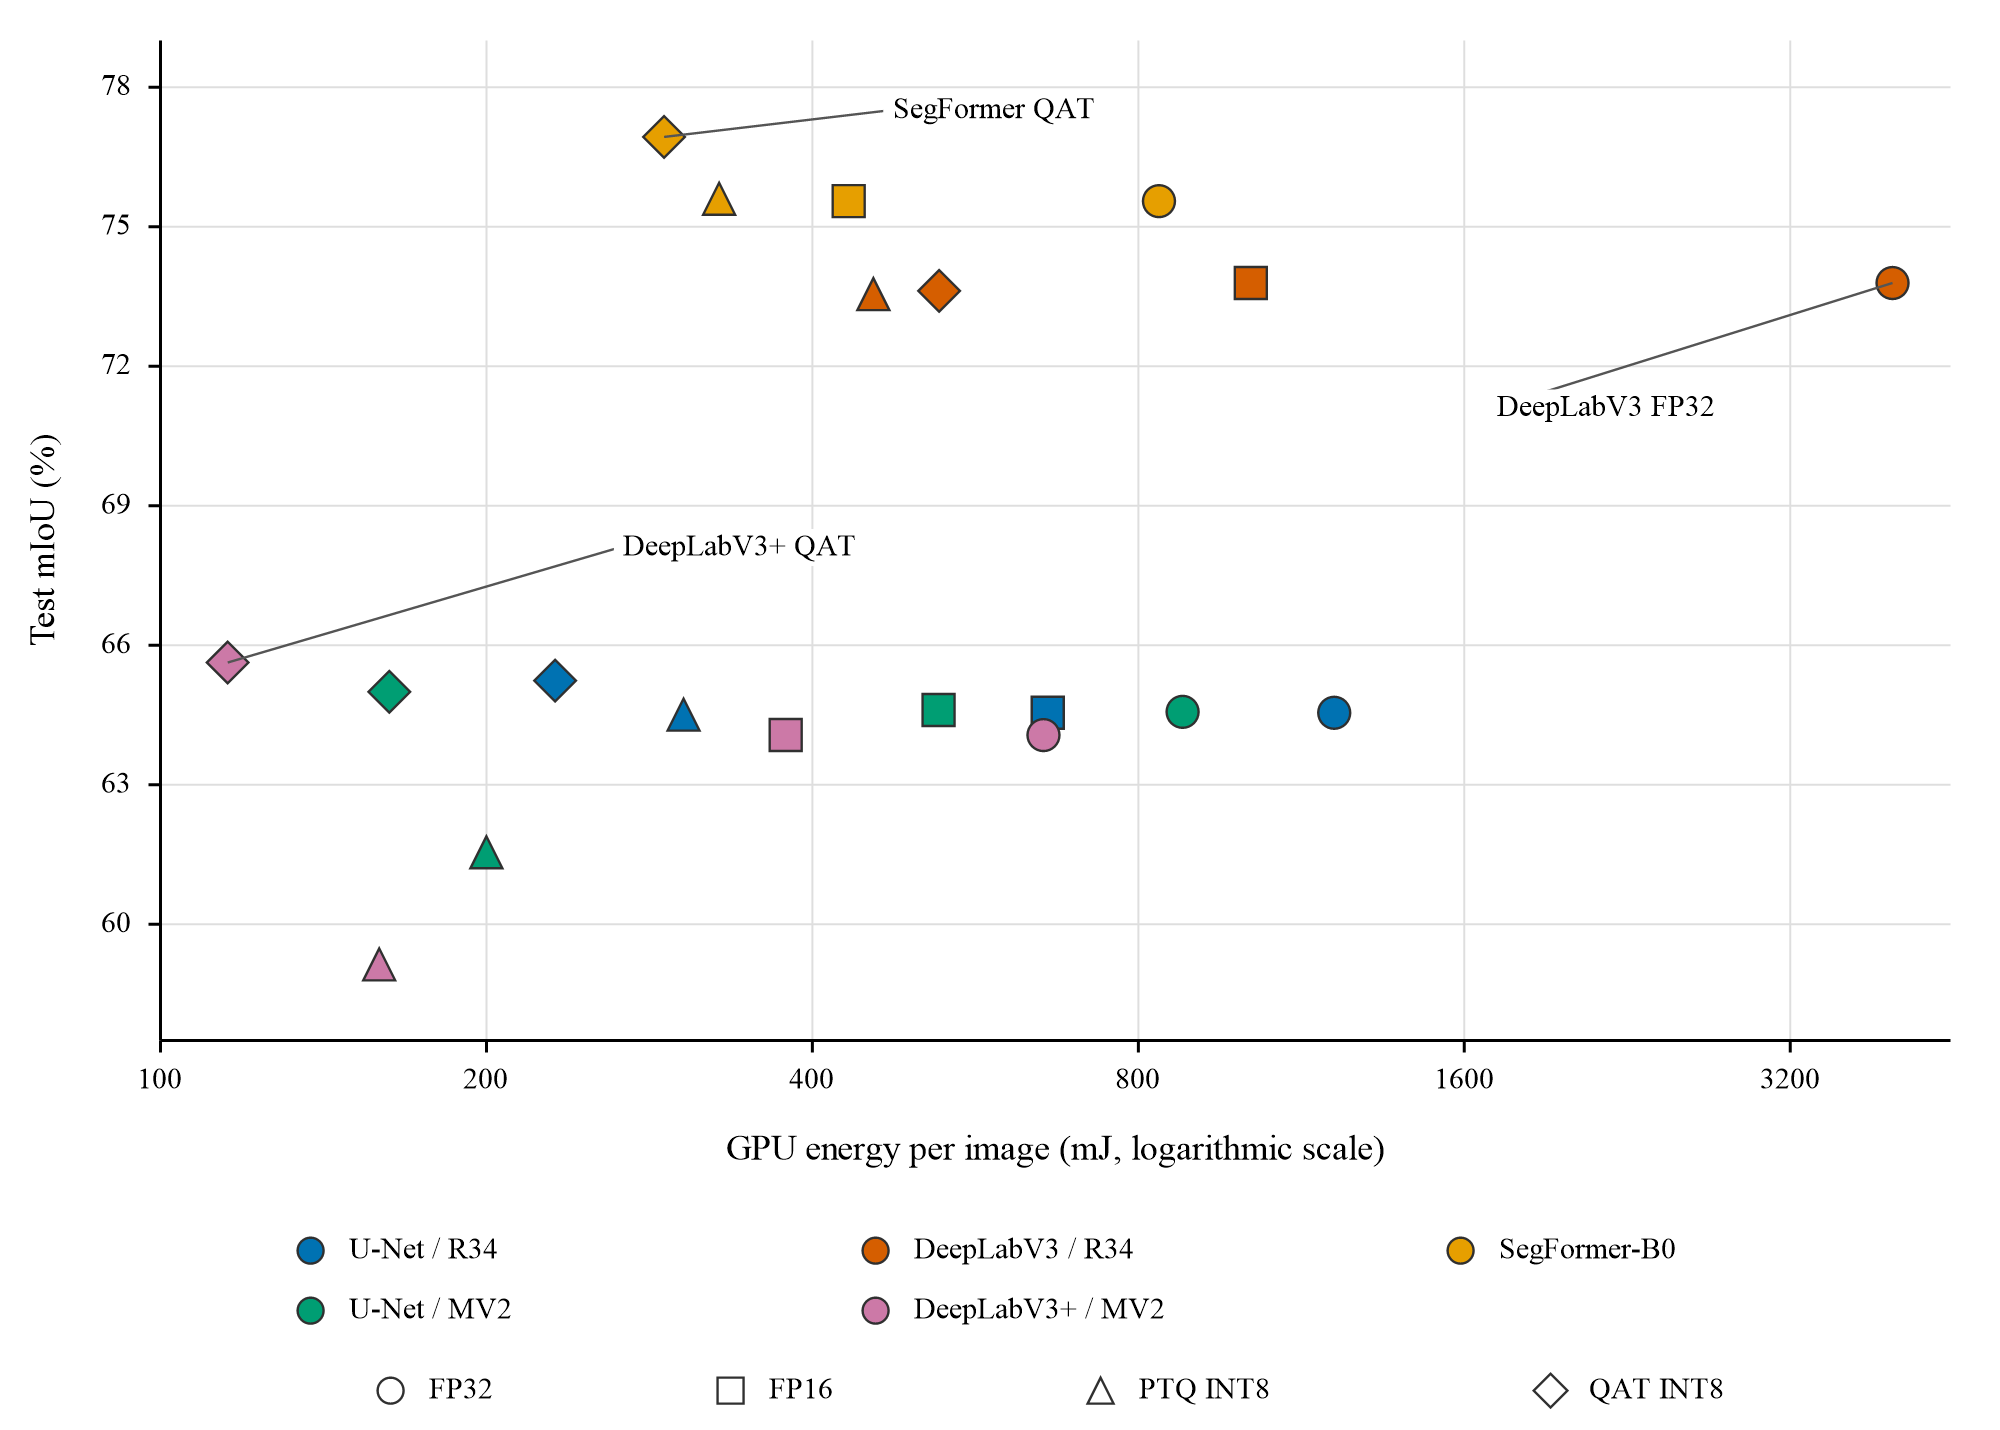
\includegraphics[width=\textwidth]{Images/quantization_miou_energy.png}
    \caption{Test mIoU versus GPU energy per image for the various configurations, with energy shown on a logarithmic scale. Colors identify the model and marker shapes identify the precision or quantization strategy. Lower energy and higher mIoU are preferable. The two QAT annotations identify the best configurations among the reported measurements, while the DeepLabV3 FP32 annotation highlights its higher energy consumption.}
    \label{fig:s5mars-quantization-miou-energy}
\end{figure}

Resource improvements were not uniform across all measurements. For U-Net with ResNet34, the QAT engine reduced latency and energy but used 1106~MiB of peak GPU memory, compared with 872~MiB for FP16. DeepLabV3 QAT also used more energy than its PTQ counterpart, 523.71 versus 455.34~mJ per image, despite its slightly higher accuracy. Since the execution backends and floating point fallback differ, these comparisons concern complete deployment configurations rather than isolating the effect of bit width. Furthermore, energy was estimated over a sustained GPU inference loop, includes device idle consumption, and excludes CPU energy. It is not an end-to-end system measurement or evidence of equivalent savings on rover flight hardware.

\section{Ablation Studies}
\label{sec:segmentation-ablation-studies}

The ablation studies investigate how the training strategy affects segmentation accuracy, providing an experimental basis for the configurations adopted in this study. The comparisons examine alternative loss formulations and class-weighting schemes, encoder initialization, data augmentation, and oversampling to assess whether these choices improve mIoU relative to their default settings. Because of time constraints, some experiments were conducted on a subset of the segmentation models evaluated in this study.

\subsection{Loss Function and Class Weighting}

% Evidence: original experiment Timeline, entries of 4 and 9 July.
% https://docs.google.com/document/d/11GTkTgIXR0t03VsOXm4SB1oaA0jJPNN3a9KFPZnC5KQ/edit
The initial loss comparison examined the combination of Cross-Entropy and Generalized Dice Loss (GDL) over Cross-Entropy alone for both SegFormer-B0 and U-Net with ResNet34, using the checkpoint with the highest validation mIoU for each run. As shown in Table~\ref{tab:s5mars-exploratory-loss-ablation}, test mIoU increased from 69.2\% to 75.5\% for SegFormer-B0 and from 59.5\% to 64.5\% for U-Net with ResNet34. These trials motivated the use of the combined objective with \(\alpha = 0.5\), which gives equal coefficients to pixel-wise classification and region-overlap supervision. Standalone GDL was also tried during preliminary experimentation but was not stable, so no numerical result is reported for that configuration.

\begin{table}[ht!]
    \centering
    \small
    \setlength{\tabcolsep}{5pt}
    \begin{tabular}{@{}l c c@{}}
        \toprule
        \textbf{Model}   & \textbf{CE} & \textbf{CE + GDL} \\
        \midrule
        \midrule
        SegFormer-B0     & 69.2        & 75.5              \\
        U-Net (R34) & 59.5        & 64.5              \\
        \bottomrule
    \end{tabular}
    \vspace{5mm}
    \caption{Approximate test mIoU (\%). CE + GDL used inverse-square Dice weights.}
    \label{tab:s5mars-exploratory-loss-ablation}
\end{table}

Class weighting was tested to assess whether increasing the Dice contribution of classes occupying fewer pixels improved segmentation accuracy. Table~\ref{tab:s5mars-exploratory-dice-weighting} compares the three GDL weighting schemes for U-Net with ResNet34. Inverse-square weighting (\texttt{square}) achieved a test mIoU of 64.5\%, compared with 62.2\% for uniform weighting and 57.2\% for inverse-class-volume weighting (\texttt{simple}). These exploratory results motivated the use of inverse-square weighting in subsequent experiments. The interaction between this weighting scheme and oversampling is examined separately below.

\begin{table}[ht!]
    \centering
    \small
    \setlength{\tabcolsep}{5pt}
    \begin{tabular}{@{}l c c c@{}}
        \toprule
        \textbf{Model}   & \textbf{Inverse square} & \textbf{Inverse volume} & \textbf{Uniform} \\
        \midrule
        \midrule
        U-Net (R34) & 64.5                    & 57.2                    & 62.2             \\
        \bottomrule
    \end{tabular}
    \vspace{5mm}
    \caption{Approximate test mIoU (\%) for U-Net with ResNet34 using CE + GDL and the three Dice-weighting schemes.}
    \label{tab:s5mars-exploratory-dice-weighting}
\end{table}

\subsection{Effect of Pretraining}

The initialization experiment assessed whether ImageNet-pretrained encoder weights provided a useful starting point for learning Martian scene segmentation. U-Net with ResNet34 trained from random initialization reached a test mIoU of 51.6\%, much below the pretrained U-Net results reported above. This observation is consistent with a benefit from pretrained initialization for the tested model and supports keeping it in subsequent experiments.

\subsection{Effect of Data Augmentation}

% Evidence: SegFormer reference and augmentation history.json/test_metrics.json.
% Reference test: Drive 1V8TqPDClr6jI39Jp7jNX3giIZM3HcoQr.
% Augmented test: Drive 1EVKdHS397eHql34tAjqcVnvNG2pIwurP.
The augmentation experiment tested whether adding transformed versions of the training images could help SegFormer-B0 perform better on unseen S5Mars images. The tested policy combined horizontal and vertical flips with random right-angle rotations. With standard sampling and inverse-square Dice weights, enabling this policy reduced validation mIoU from 80.28\% to 73.99\%, as shown in Table~\ref{tab:s5mars-segformer-training-ablation}. Test mIoU also fell from 75.55\% to 66.86\%. The extra geometric variation therefore did not improve accuracy in this experiment, therefore motivating keeping data augmentation disabled in the default configuration, while the test result shows the same pattern on unseen images.

\begin{table}[ht!]
    \centering
    \small
    \setlength{\tabcolsep}{5pt}
    \begin{tabular}{@{}l c c r r@{}}
        \toprule
        \textbf{Sampling}                              & \textbf{Dice weights} & \textbf{Augmentation} &
        \shortstack{\textbf{Val. mIoU}\\\textbf{(\%)}} &
        \shortstack{\textbf{Test mIoU}\\\textbf{(\%)}}                                                                 \\
        \midrule
        \midrule
        Standard                                       & \texttt{square}       & Disabled              & 80.28 & 75.55 \\
        Standard                                       & \texttt{square}       & Enabled               & 73.99 & 66.86 \\
        Oversampling                                   & \texttt{square}       & Disabled              & 70.64 & 71.02 \\
        Oversampling                                   & \texttt{uniform}      & Disabled              & 79.28 & 72.90 \\
        \bottomrule
    \end{tabular}
    \vspace{5mm}
    \caption{SegFormer-B0 training variants evaluated using the checkpoints with the highest validation mIoU in their respective training histories. All variants used the combined CE-GDL loss function. \texttt{square} denotes inverse-square class-volume weighting within GDL. Augmentation and oversampling were restricted to training, leaving validation and test samples unchanged.}
    \label{tab:s5mars-segformer-training-ablation}
\end{table}
% Evidence: oversampling test_metrics.json, square and uniform variants.
% Square: Drive 1s_l_TyB95OB8MKnpYZxyBpOtJ1FeOwLl.
% Uniform: Drive 1MDyDKpOWjn5CrlWKmub8_dgRWnfQ1qWH.
The oversampling experiment tested whether showing images containing rare classes more often during training could improve SegFormer-B0 accuracy on unseen S5Mars images. It also examined whether uniform Dice weights worked better than inverse-square weights when oversampling was enabled. As shown in Table~\ref{tab:s5mars-segformer-training-ablation}, oversampling with inverse-square weights produced lower validation and test mIoU than standard sampling: 70.64\% versus 80.28\% on validation and 71.02\% versus 75.55\% on test. Switching to uniform weights raised the oversampled run to 79.28\% on validation and 72.90\% on test, but both scores remained below the default. These results support keeping standard sampling with inverse-square Dice weights in the default configuration, with the validation and test scores showing the same trend. The benefit of uniform weights was observed within the oversampled runs, probably due to the work of square weights being done in part by oversampling.

%\subsection{Quantization Scope}
% TODO
% PTQ evidence: semantic_segmentation/docs/quantization/onnx_ptq_results.md,
% final SegFormer Conv+MatMul comparison (validation 200, test 800).
% QAT evidence: Conv-only Drive 1Kq-yIOds3hbGkVQPjJ8wi-uDNuhLpPyE;
% extended scope Drive 1ASZu4lePsdCcs28pVs4e_IkEoqJLd-Ge (no test result).
%The SegFormer experiments also examined how extending the INT8 scope affected segmentation accuracy. In PTQ, adding matrix multiplications to the Conv-only scope reduced test mIoU from 75.60\% to 75.12\%, as reported in Table~\ref{tab:s5mars-quantization-scope-ablation}. This deployment variant also moved convolutional biases into floating-point addition operations for TensorRT compatibility, so the comparison does not isolate the effect of quantizing matrix multiplications alone.

% \begin{table}[ht!]
%     \centering
%     \small
%     \setlength{\tabcolsep}{5pt}
%     \begin{tabular}{@{}l l r r@{}}
%         \toprule
%         \textbf{Method}                                & \textbf{INT8 scope}                                                       &
%         \shortstack{\textbf{Val. mIoU}\\\textbf{(\%)}} &
%         \shortstack{\textbf{Test mIoU}\\\textbf{(\%)}}                                                                                             \\
%         \midrule
%         \midrule
%         PTQ                                            & Convolutions only                                                         & 79.82 & 75.60 \\
%         PTQ                                            & Convolutions and matrix multiplications                                   & 79.53 & 75.12 \\
%         \midrule
%         QAT                                            & Convolutions only                                                         & 83.00 & 76.93 \\
%         QAT                                            & \shortstack[l]{Convolutions, encoder MLP\\and decoder linear projections} & 83.28 & --    \\
%         \bottomrule
%     \end{tabular}
%     \vspace{5mm}
%     \caption{SegFormer-B0 accuracy for different PTQ and QAT quantization scopes, measured on the deployed mixed-precision models rather than through fake-quantization evaluation. Unlisted operations remain floating point. The extended PTQ variant also changes convolutional bias handling. A dash denotes a test evaluation that was not performed.}
%     \label{tab:s5mars-quantization-scope-ablation}
% \end{table}

% The QAT extension instead quantized the linear layers in the encoder MLP blocks and decoder projections, while leaving attention computations in floating point. Validation mIoU increased from 83.00\% to 83.28\%. The extended configuration was not retained under the joint accuracy--efficiency selection criterion, and no held-out test result is available for it. Its validation gain therefore cannot be interpreted as an improvement in test performance over the Conv-only configuration.

\section{Cross-Mission Generalization on MarsSeg}
\label{sec:marsseg-cross-mission-generalization}

% Evidence: source test_metrics.json and cross_dataset_test JSONs from the
% six MarsSeg experiment folders, audited on 2026-10-05.
% https://drive.google.com/drive/folders/1t8bbQhbUIwbX6fOQZ45--8gfwyuhH7DS
The cross-mission experiment was designed to test whether a model trained on one rover mission could recognize the same terrain categories on another mission without additional training. This matters when labeled images from a new mission are scarce, and it also tests whether good results on the training mission translate into reliable generalization. MarsSeg MSL and MER were chosen because their Mars-Bench releases share the same terrain labels \cite{purohit2025marsbench}. S5Mars contains only Curiosity imagery and uses a different taxonomy, which would require remapping labels for a comparable cross-mission test.

SegFormer-B0, U-Net with ResNet34, and DeepLabV3+ with MobileNetV2 were each trained separately on MSL and MER. For each run, the checkpoint selected on the source validation split was tested on both the source mission and the other mission, with the same preprocessing and output labels. The cross-mission test used no target domain fine-tuning, giving a zero-shot measure of transfer. Models trained on the target mission provided a reference on the same test images, as reported in Table~\ref{tab:marsseg-cross-mission-accuracy}.

\begin{table}[ht!]
    \centering
    \small
    \setlength{\tabcolsep}{5pt}
    \begin{tabular}{@{}l r r r r@{}}
        \toprule
        \textbf{Model}                            &
        \multicolumn{2}{c}{\textbf{MSL training}} &
        \multicolumn{2}{c}{\textbf{MER training}}                                                                                 \\
        \cmidrule(lr){2-3}
        \cmidrule(l){4-5}
                                                  & \textbf{MSL test} & \textbf{MER test} & \textbf{MER test} & \textbf{MSL test} \\
        \midrule
        \midrule
        SegFormer-B0                              & 70.63             & \textbf{52.06}    & 66.75             & \textbf{48.11}    \\
        U-Net (R34)                          & \textbf{71.80}    & 27.43             & \textbf{67.76}    & 13.82             \\
        DeepLabV3+ (MV2)                  & 68.98             & 38.27             & 65.10             & 12.86             \\
        \bottomrule
    \end{tabular}
    \vspace{5mm}
    \caption{Test mIoU (\%) for the MarsSeg cross-mission experiments. Each training mission identifies a separately trained model, evaluated on both test datasets. Evaluation on the other mission is zero-shot, without target-domain fine-tuning. Bold values indicate the highest recorded mIoU in each column.}
    \label{tab:marsseg-cross-mission-accuracy}
\end{table}

In-domain results were similar across the three configurations, with U-Net ranking first on both missions. Once the mission changed, SegFormer-B0 performed substantially better than both convolutional models in both directions. The CNNs struggled especially when trained on MER and tested on MSL, while SegFormer-B0 showed a more balanced transfer across the two missions. This answers the main question of the experiment, showing that high in-domain accuracy alone did not ensure good generalization, as even SegFormer-B0 lost accuracy compared with its target trained references.

The smaller MER training split may partly explain why transfer from MER to MSL was harder for the convolutional models. With fewer examples, models may learn features that are too specific to the source images. Acquisition also differs: MSL provides RGB Mastcam images, whereas MER provides grayscale Navcam/Pancam images, and the images differ in their original dimensions \cite{purohit2025marsbench}. Such differences may make learned color or texture patterns less useful on the other mission.

SegFormer-B0's stronger transfer is consistent with its ability to combine local detail with larger scene context \cite{xie2021segformer}, together with its ADE20K segmentation pretraining. This initialization already provides features learned for pixel-level scene understanding, whereas the CNN encoders started from ImageNet classification weights, as described in Section~\ref{sec:segmentation-architectures}. Both factors may help when mission-specific training data are limited or image appearance changes. The results therefore support the evaluated Transformer configuration for cross-mission generalization.

\chapter{Evaluation of Synthetic Damage Inspection}

\section{Experimental Setup}
\label{sec:damage-experimental-setup}

The experiments used the synthetic dataset described in Section~\ref{sec:final-synthetic-dataset}, preserving its original training, validation, and test assignments when filtering by camera pose. The main comparison of PC-S, PC-L, EAD-S, SSN, TG-384, and TG-512 focused on pose A, which represents a controlled acquisition setting while retaining variations in wheel identity, lighting, and surface wear. This subset contains 2,800 normal training images, 296 normal and 96 anomalous validation images, and 404 clean-anomalous pairs in the test split, for a total of 808 test images. % A separate TinyGLASS experiment considered pose D, with 351 normal training images, 43 normal and 18 anomalous validation images, and 44 test pairs. These pose specific subsets retain different sample populations and should not be interpreted as an isolated effect of camera viewpoint.

Table~\ref{tab:damage-reference-configurations} summarizes the reference configurations using the abbreviations introduced in Chapter~4. The pose-A inputs use the fixed \(720\times720\) crop described in Section~\ref{sec:damage-preprocessing}, followed by model-specific preprocessing. The models therefore share the same image population, although their input resolutions and spatial coverage differ. % Historical PatchCore runs using all poses are kept separate from this main comparison.

\begin{table}[ht!]
    \centering
    \small
    \setlength{\tabcolsep}{4pt}
    \begin{tabular}{@{}l c c l@{}}
        \toprule
        \textbf{Configuration} & \textbf{Poses} & \textbf{Input (px)} & \textbf{Setting}             \\
        \midrule
        \midrule
        PC-S                   & A              & \(384\times512\)    & 50,000 Memory Bank           \\
        PC-L                   & A              & \(224\times224\)    & 50,000 Memory Bank           \\
        EAD-S                  & A              & \(256\times256\)    & Global calibration           \\
        SSN                    & A              & \(256\times256\)    & Top-1\% score                \\
        TG-384                 & A              & \(384\times384\)    & \(48\times48\), \(\sigma=1\) \\
        TG-512                 & A              & \(512\times512\)    & \(32\times32\), \(\sigma=4\) \\
        \bottomrule
    \end{tabular}
    \vspace{5mm}
    \caption{Reference configurations for synthetic damage inspection. TG-384 and TG-512 settings indicate the feature-grid size and Gaussian smoothing parameter.}
    \label{tab:damage-reference-configurations}
\end{table}

Both PatchCore configurations used a candidate reservoir capped at 1,000,000 descriptors, from which a memory bank of 50,000 descriptors was retained, with Gaussian smoothing set to \(\sigma=4\). After the fixed pose-A crop, PC-S resized the image directly to \(384\times512\), whereas PC-L resized the shorter side to 256 pixels before applying a \(224\times224\) center crop. Image-score reweighting used nine neighbors for PC-S and was disabled for PC-L. The SSN reference used a Perlin threshold of 0.2 without restricting synthetic perturbations to the target wheel mask. Both TG-384 and TG-512 used wheel restricted, hole like LAS perturbations, sampling small, medium, and large severities with probabilities of 70\%, 25\%, and 5\%, respectively. These probabilities apply to training perturbations, not to the composition of the rendered evaluation splits. TG-384 used layer2 features, whereas TG-512 used layer3 features, for efficiency purposes, with \(\sigma=4\) selected through a post hoc validation comparison of smoothing values.

SSN was trained with a batch size of 16 for up to 100 epochs, while TinyGLASS used batches of eight for up to 640 epochs. For these models, the checkpoint with the highest validation Image AUROC was kept and subsequently evaluated on the corresponding test split. Early stopping used a patience of five validation checks for SSN and 40 for TinyGLASS. EAD-S instead used the final checkpoint of a fixed 70,000-step run, followed by calibration on the 296 normal validation images. PatchCore constructed its memory bank once for each configuration and therefore did not require an epoch-wise checkpoint search. The test results reported in the following sections use these chosen model checkpoints and the metrics defined in Section~\ref{sec:damage-evaluation-metrics}.

Efficiency benchmarks used an NVIDIA T4 GPU in Kaggle, processing one image at a time. Latency was averaged over 50 synchronized measurements after 10 warm-up runs for prediction on an input already in GPU memory, excluding image and mask loading, preprocessing, and transfer to the GPU. Energy was measured separately during repeated prediction, with a 5-second warm-up followed by three 30-second measurement windows. NVML provided the GPU energy counter, with energy per image calculated by dividing the total GPU energy by the number of predictions across the three windows. This value covered the whole GPU, including idle consumption, and excluded CPU processing and input transfer.

\section{Model Comparison}
\label{sec:damage-model-comparison}
Table~\ref{tab:damage-reference-test-results} compares the test results of the configurations defined in Table~\ref{tab:damage-reference-configurations}, separating image-level damage detection from pixel-level localization.

% AUPRO test sources: PC-S and PC-L local extended_diagnostics.json records, 2026-10-06.
% EfficientAD-S: Drive 1yzt2Po_ygLm0tAUv8rUoJcGQiIB336XF.
% SuperSimpleNet: Drive 1xgGFz7-N5HO_jP82qnsNqK4QU6krJQtA.
% TinyGLASS (384): Drive 1WJXkAa-5P3czBlCo0WozOvPF7zj0FCgj.
% TinyGLASS (512): local test_sigma4_user_summary/test_user_summary.json, 2026-10-07.
\begin{table}[ht!]
    \centering
    \small
    \setlength{\tabcolsep}{3.5pt}
    \begin{tabular}{@{}l c c c c c c c@{}}
        \toprule
        \textbf{Configuration}                      &
        \shortstack{\textbf{Image}\\\textbf{AUROC}} &
        \shortstack{\textbf{Image}\\\textbf{AP}}    &
        \shortstack{\textbf{Pixel}\\\textbf{AUROC}} &
        \shortstack{\textbf{Pixel}\\\textbf{AP}}    &
        \shortstack{\textbf{AUPRO}\\\textbf{@0.05}} &
        \shortstack{\textbf{AUPRO}\\\textbf{@0.10}} &
        \shortstack{\textbf{AUPRO}\\\textbf{@0.30}}                                                                                                                        \\
        \midrule
        \midrule
        PC-S                                        & 79.28          & 77.49          & \textbf{99.78} & 41.05          & \textbf{94.93} & \textbf{97.35} & \textbf{99.10} \\
        PC-L                                        & \textbf{86.43} & \textbf{88.63} & 99.43          & \textbf{42.89} & 82.90          & 89.36          & 95.44          \\
        EAD-S                                       & 66.50          & 64.74          & 96.36          & 9.00           & 58.45          & 70.36          & 84.98          \\
        SSN                                         & 82.72          & 86.08          & 96.97          & 19.10          & 71.62          & 78.58          & 87.53          \\
        TG-384                                      & 77.52          & 79.28          & 97.21          & 25.48          & 73.93          & 81.10          & 90.24          \\
        TG-512                                      & 77.33          & 81.12          & 97.92          & 27.59          & 76.54          & 83.56          & 92.01          \\
        \bottomrule
    \end{tabular}
    \vspace{5mm}
    \caption{Damage detection and localization percentages on the pose-A test split. AUPRO is normalized up to the maximum FPR indicated in each column.}
    \label{tab:damage-reference-test-results}
\end{table}

PC-L achieved the highest Image AUROC and Image AP, 86.43\% and 88.63\%, followed by SSN at 82.72\% and 86.08\%. PC-S obtained a lower Image AUROC of 79.28\%, while TG-384 and TG-512 produced similar detection results, with Image AUROC values of 77.52\% for TG-384 and 77.33\% for TG-512. EAD-S remained below the other configurations on both image-level detection metrics.

The localization results distinguish the two PatchCore configurations more clearly. PC-L obtained the highest Pixel AP, 42.89\%, whereas PC-S reached the highest Pixel AUROC, 99.78\%, and AUPRO@0.30, 99.10\%, with a Pixel AP of 41.05\%. PC-L therefore provided the strongest image discrimination, while PC-S achieved better regional coverage. Within TinyGLASS, TG-512 increased Pixel AP from 25.48\% to 27.59\% and AUPRO@0.30 from 90.24\% to 92.01\%, maintaining nearly the same Image AUROC as TG-384. Both TinyGLASS configurations localized damage more effectively than SSN according to Pixel AP and AUPRO, even though SSN performed better at anomalous image-level detection. EAD-S obtained a Pixel AUROC of 96.36\% but only 9.00\% Pixel AP, showing that a high Pixel AUROC can coexist with limited localization precision.

Alongside detection and localization performance, Table~\ref{tab:damage-reference-efficiency} reports prediction latency, peak allocated GPU memory, and energy per image for the various configurations.

\begin{table}[ht!]
    \centering
    \small
    \setlength{\tabcolsep}{6pt}
    \begin{tabular}{@{}l r r r@{}}
        \toprule
        \textbf{Configuration}                                          &
        \shortstack{\textbf{Prediction}\\\textbf{latency (ms)}}         &
        \shortstack{\textbf{Peak allocated}\\\textbf{GPU memory (MiB)}} &
        \shortstack{\textbf{Energy}\\\textbf{(J/image)}}                                                                  \\
        \midrule
        \midrule
        PC-S                                                            & 101.21        & 277.53         & 6.849          \\
        PC-L                                                            & 62.89         & 385.25         & 4.116          \\
        EAD-S                                                           & 57.72         & 878.45         & 4.032          \\
        SSN                                                             & 27.54         & 219.69         & 1.939          \\
        TG-384                                                          & \textbf{5.13} & \textbf{38.72} & \textbf{0.239} \\
        TG-512                                                          & 6.29          & 55.03          & 0.369          \\
        \bottomrule
    \end{tabular}
    \vspace{5mm}
    \caption{Prediction latency, peak allocated GPU memory, and GPU energy per image, with preprocessed inputs already on the GPU. Memory includes the model and other live tensors, as reported by the PyTorch allocator.}
    \label{tab:damage-reference-efficiency}
\end{table}

TG-384 had the lowest measured cost across all three resources, requiring 5.13~ms per image, 38.72~MiB of peak GPU memory, and 0.239~J per image. TG-512 required 6.29~ms, 55.03~MiB, and 0.369~J per image, with higher Pixel AP and AUPRO and nearly the same Image AUROC. TG-384 and TG-512 therefore offer a choice between the lower resource requirements of TG-384 and the improved localization of TG-512. Both achieved better Pixel AP and AUPRO than SSN and EAD-S at a lower inference cost. This efficiency is consistent with TinyGLASS's compact architecture for edge deployment~\cite{bonazzi2026tinyglass} and our use of fixed feature pooling without a separate trainable adapter.

SSN offered an intermediate compromise for image-level detection: it reached 82.72\% Image AUROC at 27.54~ms per image, compared with 86.43\% at 62.89~ms for PC-L. These results favor TG-384 when inference resources are the main constraint, TG-512 when its localization improvement justifies the additional cost, and PC-L when detection quality has priority.

PC-S reduced peak GPU memory relative to PC-L, from 385.25 to 277.53~MiB, but required more time and energy per image. Its 101.21~ms latency and 6.849~J energy consumption were the highest measured values, so its advantage in regional coverage came with a greater inference cost. This behavior is consistent with its denser feature grid, which produces more local descriptors to compare against the memory bank. EAD-S required the largest memory peak, without a corresponding advantage in detection or localization in this comparison.

To examine how performance varies across dataset conditions, Table~\ref{tab:damage-test-subgroups} groups the test results by hole severity, lighting preset, and normal surface wear. Image AUROC describes detection within each group, while Pixel AP examines the localization of the corresponding damage regions.

\begin{table}[ht!]
    \centering
    \small
    \setlength{\tabcolsep}{3pt}
    \begin{tabular}{@{}l c l c c c c c c@{}}
        \toprule
        \textbf{Group} & \textbf{Pairs} & \textbf{Metric} & \textbf{PC-S} & \textbf{PC-L} & \textbf{EAD-S} & \textbf{SSN} & \textbf{TG-384} & \textbf{TG-512} \\
        \midrule
        \midrule
        \multicolumn{9}{@{}l}{\textit{Hole severity}}                                                                                                         \\
        Small          & 208            & Image AUROC     & 78.59         & 80.20         & 62.90          & 77.15        & 74.15           & 74.09           \\
                       &                & Pixel AP        & 33.09         & 19.76         & 3.22           & 11.28        & 16.00           & 21.13           \\[1mm]
        Medium         & 157            & Image AUROC     & 78.99         & 92.07         & 70.10          & 87.97        & 80.10           & 79.11           \\
                       &                & Pixel AP        & 44.38         & 40.22         & 14.50          & 21.14        & 30.47           & 32.98           \\[1mm]
        Large          & 39             & Image AUROC     & 85.21         & 99.80         & 71.99          & 91.91        & 84.52           & 87.18           \\
                       &                & Pixel AP        & 55.27         & 68.93         & 14.46          & 27.04        & 34.01           & 35.13           \\
        \midrule
        \multicolumn{9}{@{}l}{\textit{Lighting preset}}                                                                                                       \\
        Clear          & 97             & Image AUROC     & 82.30         & 84.71         & 67.70          & 83.61        & 79.66           & 81.29           \\
                       &                & Pixel AP        & 42.23         & 44.78         & 10.06          & 22.69        & 26.66           & 33.19           \\[1mm]
        Dusty          & 307            & Image AUROC     & 80.04         & 87.37         & 67.49          & 82.94        & 78.51           & 77.24           \\
                       &                & Pixel AP        & 43.60         & 43.30         & 11.47          & 18.38        & 28.25           & 26.66           \\
        \midrule
        \multicolumn{9}{@{}l}{\textit{Normal surface wear}}                                                                                                   \\
        Current        & 85             & Image AUROC     & 83.64         & 91.29         & 65.51          & 80.86        & 75.82           & 79.33           \\
                       &                & Pixel AP        & 42.34         & 49.25         & 9.11           & 19.36        & 18.33           & 28.78           \\[1mm]
        Light wear     & 179            & Image AUROC     & 77.47         & 84.71         & 66.50          & 82.50        & 77.95           & 77.42           \\
                       &                & Pixel AP        & 39.92         & 39.48         & 8.70           & 19.76        & 28.24           & 26.46           \\[1mm]
        Evident wear   & 140            & Image AUROC     & 79.22         & 85.48         & 67.21          & 84.33        & 77.88           & 76.69           \\
                       &                & Pixel AP        & 43.19         & 45.48         & 11.25          & 18.41        & 27.38           & 29.24           \\
        \bottomrule
    \end{tabular}
    \vspace{5mm}
    \caption{Test subgroup results (\%) by hole severity, lighting, and surface wear, with clean-anomalous pair counts. Current denotes the surface without additional wear.}
    \label{tab:damage-test-subgroups}
\end{table}

Hole severity produced the clearest common trend: all six configurations achieved higher Image AUROC on large holes than on small holes. PC-L showed the strongest separation, increasing from 80.20\% for small holes to 92.07\% and 99.80\% for medium and large holes. Larger perforations occupy more of the visible wheel surface and are likely to retain a clearer anomaly signal after resizing and feature extraction. Small holes remain more difficult to distinguish from normal local texture, although PC-S preserved the highest Pixel AP on this group, 33.09\%, followed by TG-512 at 21.13\%. Both exceeded PC-L's 19.76\%, so PC-L's higher aggregate Pixel AP is largely due to better localization of larger anomalous regions. TG-512 also improved Pixel AP over TG-384 at every severity, with the largest gain on small holes, from 16.00\% to 21.13\%. Pixel AP was higher for medium and large holes than for small holes across all six configurations, with part of this difference reflecting the greater proportion of anomalous pixels in larger defects.

Lighting had a less uniform effect. SSN obtained a Pixel AP of 22.69\% under the clear preset and 18.38\% under the dusty preset. TG-512's Image AUROC decreased from 81.29\% to 77.24\%, while its Pixel AP decreased from 33.19\% to 26.66\%. These differences are compatible with dust and illumination changes reducing the visual distinction between a perforation and the surrounding surface. Other configurations kept similar scores or improved on the dusty subgroup, therefore not representing a uniformly harder condition across the evaluated models.

Normal wear also affected the models differently. PC-L achieved its highest Image AUROC without additional wear, 91.29\%, compared with 84.71\% under light wear and 85.48\% under evident wear. PC-S followed the same detection trend, which is consistent with scratches introducing local appearance changes that can resemble damage in feature matching. SSN instead had Image AUROC values between 80.86\% and 84.33\% across the three surface conditions, while TG-384 achieved higher Pixel AP under light and evident wear than without additional wear. TG-512's Pixel AP ranged from 26.46\% under light wear to 29.24\% under evident wear, with 28.78\% without additional wear. The synthesis-based models may benefit from learning to distinguish local perturbations from the varied normal textures represented during training, although the observed wear results do not follow a common monotonic pattern.

Figure~\ref{fig:damage-model-map-comparison} compares the six reference configurations on the same damaged wheel image. All models show a local peak in anomaly score near the perforation, although its contrast with the surrounding wheel varies. Converting these continuous maps into damage masks requires a suitable threshold for each model to retain the defect response while suppressing lower scores on normal regions. This is particularly important for PatchCore and EAD-S, whose maps also show widespread responses beyond the anomalous region. Normal structural openings in the wheel make this distinction more difficult, since both these openings and damage holes can reveal dark interior regions.

\begin{figure}[ht!]
    \centering
    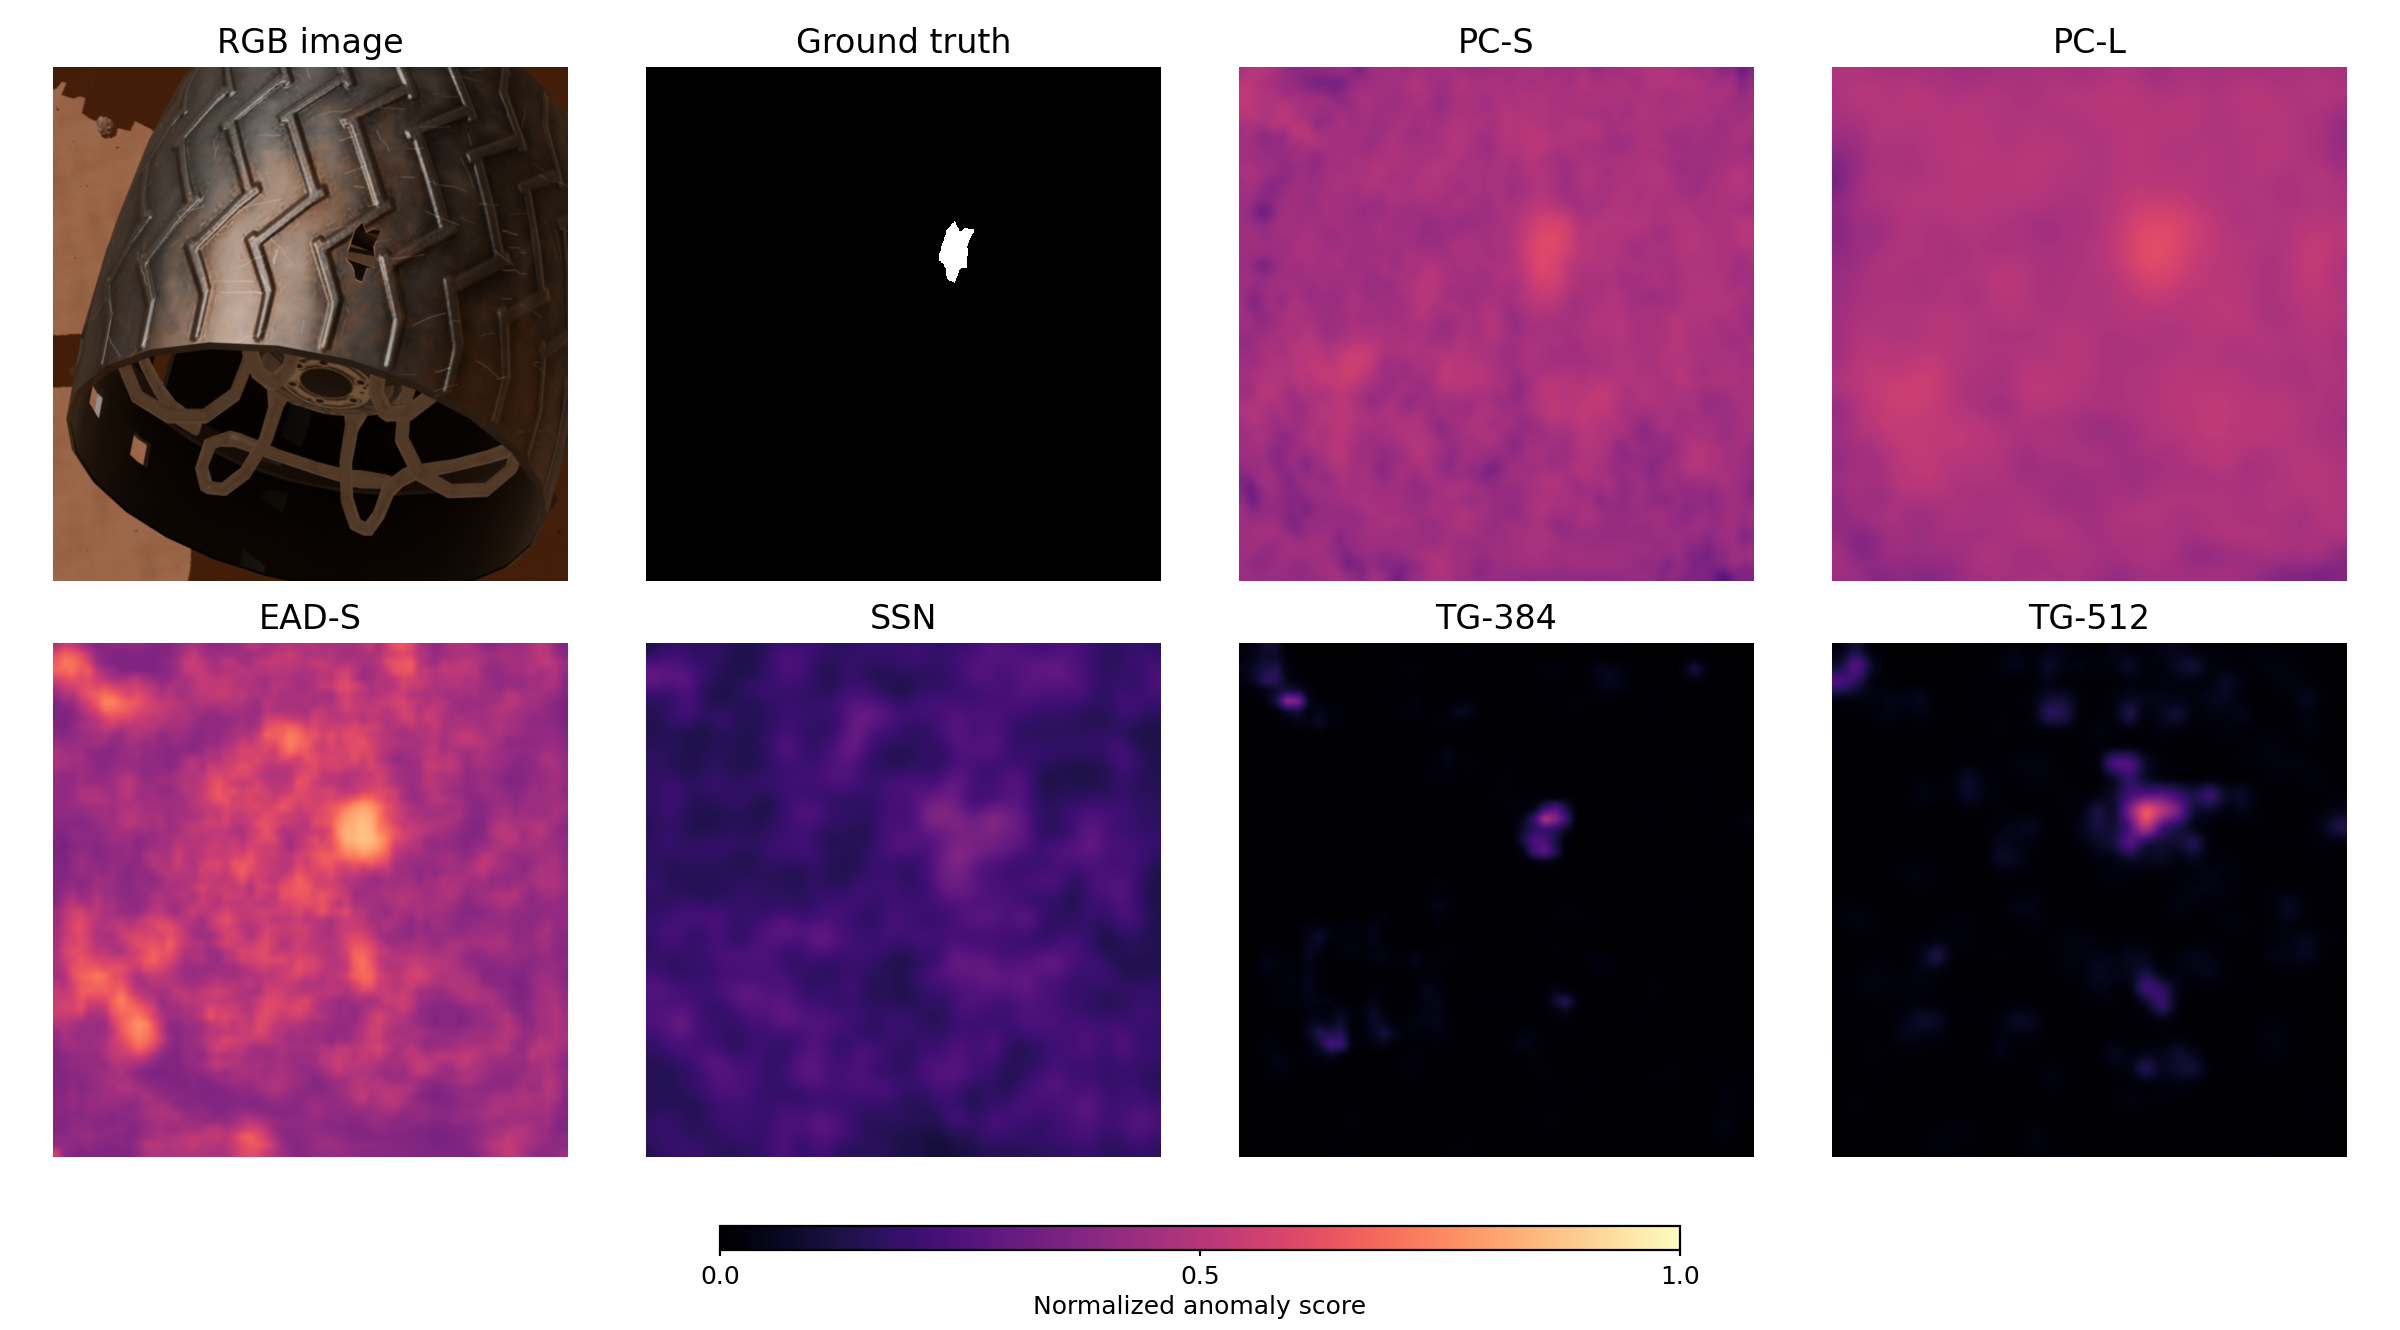
\includegraphics[width=\textwidth]{Images/damage_model_prediction_comparison.png}
    \vspace{5mm}
    \caption{Qualitative comparison of the RGB image, ground truth damage mask, and normalized anomaly maps for the six reference configurations.}
    \label{fig:damage-model-map-comparison}
\end{figure}
\FloatBarrier

\section{Ablation Studies}
\label{sec:damage-ablation-studies}

The following experiments examined which changes improved damage detection and localization within each model family. The comparisons explain the choices used in the chosen configurations, considering the representation of normal appearance, the training perturbations, and the spatial detail available for small perforations.

\subsection{Memory Bank and Smoothing in PatchCore}
\label{sec:damage-patchcore-ablation}

PatchCore was the first anomaly detector analyzed, and these experiments were conducted using all camera poses, before the study adopted pose A as the common experimental setting. The memory bank size and smoothing studied in this stage were subsequently used for pose A experiments. The pose A comparison therefore used only the best configuration found.

The memory-bank comparison tested whether storing more examples of normal wheel appearance would improve detection and localization enough to justify the additional memory required to store the bank. The candidate reservoir was fixed at 1,000,000 descriptors, while the bank size varied as shown in Table~\ref{tab:damage-patchcore-bank-ablation}. For the PC-S configuration, increasing the bank from 20,000 to 50,000 descriptors improved both validation Image AUROC and Pixel AP. A further increase to 100,000 doubled the storage without improving either validation metric. The PC-L preset showed a similar trade-off: 100,000 descriptors slightly improved validation Image AUROC, but reduced Pixel AP and required twice the bank memory. These results supported keeping 50,000 descriptors for both configurations, with the test results showing little benefit from the larger bank.

\begin{table}[ht!]
    \centering
    \small
    \setlength{\tabcolsep}{3pt}
    \begin{tabular}{@{}l r c c c c r@{}}
        \toprule
        \textbf{Preset} & \textbf{Bank} & \multicolumn{2}{c}{\textbf{Validation (\%)}} & \multicolumn{2}{c}{\textbf{Test (\%)}} & \shortstack{\textbf{Bank}\\\textbf{(MiB)}}                              \\
                        &               & \textbf{Image AUROC}                         & \textbf{Pixel AP}                      & \textbf{Image AUROC}                       & \textbf{Pixel AP} &        \\
        \midrule
        \midrule
        PC-S            & 20,000        & 78.51                                        & 21.59                                  & 70.91                                      & 26.96             & 29.30  \\
        PC-S            & 50,000        & 81.89                                        & 22.68                                  & 72.81                                      & 27.56             & 73.24  \\
        PC-S            & 100,000       & 81.36                                        & 22.60                                  & 72.94                                      & 27.89             & 146.48 \\
        \midrule
        PC-L            & 50,000        & 89.73                                        & 31.39                                  & 77.94                                      & 30.95             & 195.31 \\
        PC-L            & 100,000       & 89.94                                        & 29.48                                  & 77.58                                      & 30.43             & 390.63 \\
        \bottomrule
    \end{tabular}
    \vspace{5mm}
    \caption{PatchCore bank comparison using all poses, with a reservoir of 1,000,000 descriptors and \(\sigma=4\). PC-S uses a \(512\times512\) input and PC-L a \(224\times224\) input. Memory refers to the bank alone.}
    \label{tab:damage-patchcore-bank-ablation}
\end{table}

Gaussian smoothing was examined separately to test whether reducing isolated high anomaly scores in the map would improve localization while preserving image-level detection. This comparison used the PC-S configuration with a bank of 100,000 descriptors. Table~\ref{tab:damage-patchcore-smoothing-ablation} shows that \(\sigma=4\) produced the highest Pixel AP on both splits, while test Image AUROC remained identical across the three settings. The result supports smoothing as a way to improve the spatial distribution of anomaly scores, and \(\sigma=4\) was kept for the subsequent PatchCore runs.

\begin{table}[ht!]
    \centering
    \begin{tabular}{@{}c c c c@{}}
        \toprule
        \textbf{\(\sigma\)} & \textbf{Val Pixel AP} & \textbf{Test Pixel AP} & \textbf{Test Image AUROC} \\
        \midrule
        \midrule
        0                   & 20.15                 & 24.75                  & 72.61                     \\
        1                   & 20.57                 & 25.16                  & 72.61                     \\
        4                   & 23.05                 & 27.69                  & 72.61                     \\
        \bottomrule
    \end{tabular}
    \vspace{5mm}
    \caption{Smoothing comparison (\%) for the PC-S run using all poses with 100,000 descriptor bank.}
    \label{tab:damage-patchcore-smoothing-ablation}
\end{table}

\subsection{Calibration and Scoring in EAD-S}
\label{sec:damage-efficientad-ablation}

The EAD-S experiments tested whether accounting for the normal response at each image position could reduce false anomaly responses from the surrounding scene and normal wheel structure. Spatial calibration used normal images to normalize the anomaly scores separately at each image position. It was combined with a static wheel region, and the image score was varied to examine whether averaging a small set of high responses would be more stable than taking the maximum. These scoring candidates were evaluated on the same run using validation Image AUROC.

Table~\ref{tab:damage-efficientad-score-ablation} shows that spatial scoring improved validation discrimination over the global maximum. Averaging the highest 0.05\% of responses within the wheel region gave the highest Image AUROC, although its result was almost identical to the spatial maximum. Increasing the averaging fraction reduced Image AUROC slightly, suggesting that the strongest local responses carried most of the useful detection signal.

\begin{table}[ht!]
    \centering
    \small
    \setlength{\tabcolsep}{4pt}
    \begin{tabular}{@{}l c c c c c c@{}}
        \toprule
                        & \shortstack{\textbf{Global}\\\textbf{max}} & \shortstack{\textbf{Spatial}\\\textbf{max}} & \shortstack{\textbf{Top}\\\textbf{0.05\%}} & \shortstack{\textbf{Top}\\\textbf{0.1\%}} & \shortstack{\textbf{Top}\\\textbf{0.25\%}} & \shortstack{\textbf{Top}\\\textbf{0.5\%}} \\
        \midrule
        \midrule
        Val Image AUROC & 80.22                                      & 84.98                                       & 85.00                                      & 84.93                                     & 84.83                                      & 84.64                                     \\
        \bottomrule
    \end{tabular}
    \vspace{5mm}
    \caption{EAD-S validation scoring comparison percentages for the spatial-calibration experiment. Top fractions denote averaging within the static wheel region.}
    \label{tab:damage-efficientad-score-ablation}
\end{table}

The complete spatial and global training strategies were also compared to determine whether the improvement in validation detection was accompanied by better damage localization. The spatial strategy reserved normal training images for calibration, while the global strategy used all normal training images and calibrated after training on normal validation images. Both runs used pose A, the \(720\times720\) crop, and a fixed 70,000-step budget.

As shown in Table~\ref{tab:damage-efficientad-calibration-ablation}, the spatial strategy achieved higher validation Image AUROC, but the global strategy produced much higher validation Pixel AP. The test results showed the same localization advantage and also favored the global strategy for image-level detection. These results support the chosen global configuration as a compromise between detection and localization. One possible explanation is that position specific normalization is more sensitive to changes in lighting and surface appearance, whereas global calibration applies a common scale across image positions.

\begin{table}[ht!]
    \centering
    \small
    \setlength{\tabcolsep}{4pt}
    \begin{tabular}{@{}l c c c c@{}}
        \toprule
        \textbf{Strategy}   & \multicolumn{2}{c}{\textbf{Validation (\%)}} & \multicolumn{2}{c}{\textbf{Test (\%)}}                                            \\
                            & \textbf{Image AUROC}                         & \textbf{Pixel AP}                      & \textbf{Image AUROC} & \textbf{Pixel AP} \\
        \midrule
        \midrule
        Spatial, top 0.05\% & 85.00                                        & 5.44                                   & 61.37                & 2.90              \\
        Global, max         & 81.23                                        & 15.21                                  & 66.50                & 9.00              \\
        \bottomrule
    \end{tabular}
    \vspace{5mm}
    \caption{Comparison of the complete EAD-S calibration and training strategies on pose A.}
    \label{tab:damage-efficientad-calibration-ablation}
\end{table}

\subsection{Training and Scoring in SSN}
\label{sec:damage-supersimplenet-ablation}

The SSN experiments explored whether adopting a single canonical camera pose could simplify wheel inspection by reducing variations in normal appearance. Since the models learn from clean images, a more consistent view could make it easier to distinguish localized damage from changes due to viewpoint. Pose A was therefore tested alongside the setting using all poses, and a fixed crop before resizing was introduced to examine whether giving the wheel more of the input image would preserve useful damage detail and reduce the influence of the background. Table~\ref{tab:damage-ssn-acquisition-ablation} compares the four pose and crop combinations at \(256\times256\). The pose specific comparisons describe different image populations, while the crop comparison within each population shows the effect of concentrating the input on the wheel.

Pose A with cropping achieved the highest Image AUROC and Pixel AP in this comparison. Cropping was particularly useful for localization on pose A, increasing test Pixel AP from 7.27\% to 19.49\%. The modest detection improvement from cropping the inputs from all poses also indicates that removing background alone did not resolve the difficulty introduced by different views. Together, these results support the controlled pose A acquisition and cropped input used for the SSN configuration and subsequent experiments with the other models.

\begin{table}[ht!]
    \centering
    \small
    \setlength{\tabcolsep}{5pt}
    \begin{tabular}{@{}l c c c c@{}}
        \toprule
        \textbf{Metric}  & \shortstack{\textbf{All poses}\\\textbf{No crop}} & \shortstack{\textbf{All poses}\\\textbf{Crop}} & \shortstack{\textbf{Pose A}\\\textbf{No crop}} & \shortstack{\textbf{Pose A}\\\textbf{Crop}} \\
        \midrule
        \midrule
        Val Image AUROC  & 56.63                                             & 59.15                                          & 77.64                                          & 84.07                                       \\
        Val Pixel AP     & 8.77                                              & 11.62                                          & 9.18                                           & 18.44                                       \\
        Test Image AUROC & 54.05                                             & 54.95                                          & 65.26                                          & 69.74                                       \\
        Test Pixel AP    & 8.33                                              & 11.40                                          & 7.27                                           & 19.49                                       \\
        \bottomrule
    \end{tabular}
    \vspace{5mm}
    \caption{SSN acquisition comparison (\%) at \(256\times256\), before changing the image score formulation.}
    \label{tab:damage-ssn-acquisition-ablation}
\end{table}

The number of training epochs was extended to test whether the initial configuration needed more optimization, and the input was increased to \(384\times384\) to test whether additional spatial detail would improve localization. Table~\ref{tab:damage-ssn-training-ablation} shows that neither change improved validation image discrimination. At 200 epochs, the larger input increased test AUPRO but reduced Pixel AP, so its larger regional coverage came with less precise pixel-level localization. The 100 epoch setting with \(256\times256\) input size was chosen as the basis for the subsequent scoring and perturbation experiments.

\begin{table}[ht!]
    \centering
    \small
    \setlength{\tabcolsep}{4pt}
    \begin{tabular}{@{}c c c c c c@{}}
        \toprule
        \textbf{Input}   & \shortstack{\textbf{Epochs}} & \shortstack{\textbf{Val Image}\\\textbf{AUROC}} & \shortstack{\textbf{Val}\\\textbf{Pixel AP}} & \shortstack{\textbf{Test}\\\textbf{Pixel AP}} & \shortstack{\textbf{Test}\\\textbf{AUPRO@0.30}} \\
        \midrule
        \midrule
        \(256\times256\) & 100                          & 84.07                                           & 18.44                                        & 19.49                                         & 88.98                                      \\
        \(256\times256\) & 200                          & 74.55                                           & 20.81                                        & 20.62                                         & 87.19                                      \\
        \(384\times384\) & 200                          & 70.71                                           & 17.17                                        & 16.88                                         & 91.59                                      \\
        \bottomrule
    \end{tabular}
    \vspace{5mm}
    \caption{SSN number of epochs and input resolution comparisons on cropped pose A images.}
    \label{tab:damage-ssn-training-ablation}
\end{table}

The image score was then reconsidered because a small localized hole may produce a useful anomaly map without a strong response from the learned classification head. The same checkpoint was therefore evaluated using the mean of the highest 1\% of responses on the native map. Table~\ref{tab:damage-ssn-score-ablation} shows an improvement in both image metrics on validation and test, while the maps and localization metrics remained unchanged. This experiment supported using the map-based score in the subsequent SSN training runs.

\begin{table}[ht!]
    \centering
    \small
    \begin{tabular}{@{}l c c c c@{}}
        \toprule
        \textbf{Image score} & \multicolumn{2}{c}{\textbf{Validation}} & \multicolumn{2}{c}{\textbf{Test}}                                \\
                             & \textbf{AUROC}                          & \textbf{AP}                       & \textbf{AUROC} & \textbf{AP} \\
        \midrule
        \midrule
        Classification head  & 84.07                                   & 66.67                             & 69.74          & 72.45       \\
        Top 1\% mean         & 92.07                                   & 84.45                             & 81.11          & 84.72       \\
        \bottomrule
    \end{tabular}
    \vspace{5mm}
    \caption{Image-score comparison on the same SSN run, without retraining.}
    \label{tab:damage-ssn-score-ablation}
\end{table}

The synthetic perturbations were also varied to test how their extent and location affected learning. Restricting Perlin perturbations to the target wheel was intended to focus training on the structure being inspected. Within this setting, lowering the Perlin threshold from 0.6 to 0.2 tested whether a larger perturbed region would provide a stronger training signal. The high-threshold run produced weak detection and localization, whereas the lower threshold substantially improved both (Table~\ref{tab:damage-ssn-perturbation-ablation}). A plausible explanation is that the combination of a high threshold and wheel restriction left too little useful anomalous content on the feature grid.

Removing the wheel restriction at threshold 0.2 tested whether perturbations over a wider range of normal features would improve pixel discrimination. Validation Pixel AP increased from 15.45\% to 18.49\%, and test Pixel AP increased from 16.78\% to 19.10\%. Image-level detection decreased slightly, as did test AUPRO, indicating a compromise between precision and regional coverage. The unrestricted variant was chosen for its stronger localization precision.

\begin{table}[ht!]
    \centering
    \small
    \setlength{\tabcolsep}{4pt}
    \begin{tabular}{@{}c c c c c c@{}}
        \toprule
        \shortstack{\textbf{Perlin}\\\textbf{threshold}} & \shortstack{\textbf{Wheel}\\\textbf{restriction}} & \shortstack{\textbf{Val Image}\\\textbf{AUROC}} & \shortstack{\textbf{Val}\\\textbf{Pixel AP}} & \shortstack{\textbf{Test Image}\\\textbf{AUROC}} & \shortstack{\textbf{Test}\\\textbf{Pixel AP}} \\
        \midrule
        \midrule
        0.6                                              & Yes                                               & 54.69                                           & 0.20                                         & 55.73                                            & 0.29                                          \\
        0.2                                              & Yes                                               & 94.07                                           & 15.45                                        & 83.13                                            & 16.78                                         \\
        0.2                                              & No                                                & 93.35                                           & 18.49                                        & 82.72                                            & 19.10                                         \\
        \bottomrule
    \end{tabular}
    \vspace{5mm}
    \caption{SSN perturbation comparisons (\%) on cropped pose A inputs, using the top-1\% image score and \(\sigma=4\). Wheel restriction applies to training perturbations.}
    \label{tab:damage-ssn-perturbation-ablation}
\end{table}

Finally, smoothing was checked to determine whether it could improve spatial consistency without affecting the selected image score. The validation sweep over \(\sigma=0,1,2,4\) favored \(\sigma=4\) for both restricted and unrestricted perturbations, using Pixel AP for selection. Image metrics remained unchanged because the score was computed before smoothing. This supported using \(\sigma=4\) in the final SSN configuration.

\subsection{Task Adaptation and Spatial Resolution in TinyGLASS}
\label{sec:damage-tinyglass-ablation}

The first TinyGLASS experiment tested whether the constraints used to create artificial anomalies helped the model detect wheel damage. With the hypersphere constraint enabled, altered features were kept within a set distance range from a single center representing normal appearance. This constraint was removed to test whether using that common center limited the training examples that the model could learn from. GAS was still used, with local limits on the distance between each perturbed feature and its original normal feature. With the \(900\times900\) crop, removing the hypersphere constraint improved Pixel AP on both validation and test, as shown in Table~\ref{tab:damage-tinyglass-training-ablation}, supporting its removal from the subsequent configurations.

At the selected \(720\times720\) crop, LAS texture perturbations were compared with irregular, darkened hole like regions restricted to the target wheel. This experiment tested whether training anomalies closer to the appearance of the target defect would improve detection and localization. The hole variant improved both Image AUROC and Pixel AP on validation and test, supporting the use of these task specific perturbations.

\begin{table}[ht!]
    \centering
    \small
    \setlength{\tabcolsep}{3pt}
    \begin{tabular}{@{}c l c c c c@{}}
        \toprule
        \shortstack{\textbf{Crop}\\\textbf{(px)}} & \textbf{Training setting} & \multicolumn{2}{c}{\textbf{Validation (\%)}} & \multicolumn{2}{c}{\textbf{Test (\%)}}                                            \\
                                                  &                           & \textbf{Image AUROC}                         & \textbf{Pixel AP}                      & \textbf{Image AUROC} & \textbf{Pixel AP} \\
        \midrule
        \midrule
        900                                       & Texture, hypersphere      & 68.31                                        & 1.62                                   & 56.33                & 1.41              \\
        900                                       & Texture, local            & 75.40                                        & 6.39                                   & 63.81                & 7.32              \\
        \midrule
        720                                       & Texture, local            & 76.77                                        & 8.38                                   & 66.78                & 6.97              \\
        720                                       & Hole, initial             & 80.60                                        & 9.01                                   & 69.72                & 11.46             \\
        720                                       & Hole, 50/40/10\%          & 83.35                                        & 14.40                                  & 72.04                & 14.71             \\
        720                                       & Hole, 70/25/5\%           & 83.74                                        & 15.18                                  & 72.55                & 14.67             \\
        \bottomrule
    \end{tabular}
    \vspace{5mm}
    \caption{TinyGLASS training variants on pose A, using a \(256\times256\) input, the \(32\times32\) grid, and \(\sigma=4\). Local denotes the setting without the hypersphere constraint. The hole percentages refer to small, medium, and large perturbations.}
    \label{tab:damage-tinyglass-training-ablation}
\end{table}

The comparison of the size of perturbations varied the LAS probabilities for small, medium, and large perturbations from 50\%, 40\%, and 10\% to 70\%, 25\%, and 5\%. The aim was to test whether showing the model more small synthetic defects during training would improve their localization. Validation Image AUROC and Pixel AP improved modestly, but test Pixel AP remained almost unchanged, and small hole Pixel AP decreased from 7.21\% to 6.84\%. The revised distribution was kept for its validation performance, but the result showed that perturbation frequency alone did not resolve the difficulty of small defects.

Image score aggregation was tested to check whether averaging high patch responses or using a quantile could suppress the effects of an outlier without losing sensitivity to small holes. On the LAS hole checkpoint, the maximum achieved validation Image AUROC of 80.60\% and Image AP of 59.51\%. Averaging the three highest responses gave an almost identical Image AUROC of 80.55\%, but lower Image AP of 58.91\%, while wider averages and the tested quantiles performed worse, motivating the use of the maximum.

The resolution experiments also examined the trade-off between accuracy and computational cost, testing whether the additional detail from larger inputs justified the extra processing required. Larger images could preserve small perforations more clearly, but increased the work done by the backbone. Both layer2 and layer3 features were used throughout, with either interpolation to the denser layer2 grid or pooling to the coarser layer3 grid. This comparison tested whether fewer patches could reduce the work done by the discriminator while preserving useful damage information. Table~\ref{tab:damage-tinyglass-spatial-ablation} reports the resulting detection and localization metrics.

\begin{table}[ht!]
    \centering
    \small
    \setlength{\tabcolsep}{3pt}
    \begin{tabular}{@{}c c c c c c c@{}}
        \toprule
        \textbf{Input}   & \textbf{Final Resolution} & \textbf{\(\sigma\)} & \shortstack{\textbf{Val Image}\\\textbf{AUROC}} & \shortstack{\textbf{Val}\\\textbf{Pixel AP}} & \shortstack{\textbf{Test Image}\\\textbf{AUROC}} & \shortstack{\textbf{Test}\\\textbf{Pixel AP}} \\
        \midrule
        \midrule
        \(256\times256\) & layer2, \(32\times32\)    & 1                   & 83.74                                           & 16.53                                        & 72.55                                            & 15.72                                         \\
        \(384\times384\) & layer2, \(48\times48\)    & 1                   & 88.36                                           & 26.05                                        & 77.52                                            & 25.48                                         \\
        \(384\times384\) & layer3, \(24\times24\)    & 1                   & 87.58                                           & 25.98                                        & 76.91                                            & 24.18                                         \\
        \(384\times384\) & layer3, \(24\times24\)    & 4                   & 87.58                                           & 26.48                                        & 76.91                                            & 24.57                                         \\
        \(512\times512\) & layer2, \(64\times64\)    & 1                   & 83.16                                           & 24.08                                        & 73.81                                            & 23.55                                         \\
        \(512\times512\) & layer2, \(64\times64\)    & 4                   & 83.16                                           & 24.56                                        & 73.81                                            & 24.07                                         \\
        \(512\times512\) & layer3, \(32\times32\)    & 1                   & 85.57                                           & 28.26                                        & 77.33                                            & 27.01                                         \\
        \(512\times512\) & layer3, \(32\times32\)    & 4                   & 85.57                                           & 28.84                                        & 77.33                                            & 27.59                                         \\
        \bottomrule
    \end{tabular}
    \vspace{5mm}
    \caption{TinyGLASS input, grid, and smoothing comparisons on pose A with the \(720\times720\) crop and LAS hole probabilities of 70\%, 25\%, and 5\%. Image AUROC is shared by smoothing variants of the same checkpoint.}
    \label{tab:damage-tinyglass-spatial-ablation}
\end{table}

With \(\sigma=1\) and layer2 alignment, increasing the input from \(256\times256\) to \(384\times384\) improved detection and localization, with a relative increase of 62.1\% in test Pixel AP. A further increase to \(512\times512\) reduced test Pixel AP by 7.6\%. Pooling to the layer3 grid reduced the number of patches to one quarter, with test Pixel AP decreasing by 5.1\% at \(384\times384\) but increasing by 14.7\% at \(512\times512\). The higher resolution was therefore useful when combined with pooling, which may reduce the influence of normal texture while retaining damage information. The reduced patch count lowers discriminator work and feature storage, while the backbone continues to process the full input.

Smoothing was compared on the same checkpoints to assess whether localization could improve without further training. The validation sweep at \(256\times256\) with layer2 alignment favored \(\sigma=1\) for regional coverage, so this setting was carried forward to TG-384. Increasing smoothing to \(\sigma=4\) produced small gains in validation and test Pixel AP for the \(384\times384\) layer3 grid and both \(512\times512\) grids. The \(512\times512\) configuration with layer3 alignment achieved the highest validation and test Pixel AP among the settings shown, with a further relative gain of about 2\% on test after stronger smoothing. Image-level detection remained unchanged because its score was computed on the native patch grid before smoothing. Together with the resource measurements in Table~\ref{tab:damage-reference-efficiency}, these results support retaining TG-384 for its lower computational cost and TG-512 for its stronger localization.

\chapter{Discussion and Limitations}

\section{Main Findings}

\subsection{Lightweight Scene Understanding}

Among the evaluated deployment configurations, QAT SegFormer-B0 achieved the highest test mIoU, while QAT DeepLabV3+ with MobileNetV2 required the least GPU energy per image (Section~\ref{sec:quantization-results}). These configurations therefore represent the best observed accuracy-energy trade-offs: SegFormer-B0 favored segmentation quality, whereas DeepLabV3+ required less energy at the cost of lower accuracy. In the FP32 comparison, SegFormer-B0 exceeded DeepLabV3+ with MobileNetV2 by 11.48 percentage points of mIoU while requiring approximately 28\% more measured GPU energy per image. Against FP32 DeepLabV3 with ResNet34, the same FP32 SegFormer-B0 configuration achieved a relative mIoU advantage of approximately 2.4\% while consuming approximately 79\% less energy. These comparisons show that a compact Transformer configuration can provide competitive efficiency alongside accurate segmentation, although its advantage depends on the convolutional model considered. The preferred configuration consequently depends on the segmentation quality required by the application and the available energy budget.

The selected QAT configurations reduced measured GPU energy per image relative to their corresponding FP32 baselines by approximately 65\% for SegFormer-B0 and 82\% for DeepLabV3+ with MobileNetV2. Within this QAT comparison, SegFormer-B0 retained an mIoU advantage of 11.30 percentage points over DeepLabV3+ with MobileNetV2, but required approximately 153\% more energy. Its INT8 conversion was restricted to convolutions, leaving many parameters and the attention computations in FP16 to limit the risk of numerical degradation. This selective scope may partly explain the remaining inference cost. QAT also increased mIoU relative to FP32 by approximately 1.8\% and 2.4\% for SegFormer-B0 and DeepLabV3+, respectively, although these improvements resulted from a procedure that included fine-tuning and distillation. PTQ instead essentially preserved SegFormer-B0's accuracy but reduced DeepLabV3+ mIoU by approximately 7.7\% relative to FP32, confirming that accuracy preservation must be verified for each configuration. Whether the remaining energy difference is acceptable also depends on inference frequency and the available energy.

The remaining inference cost also illustrates why parameter count alone is not a reliable efficiency indicator. SegFormer-B0's attention operations and intermediate feature maps introduce computation and storage requirements that its lower parameter count does not capture, consistent with its higher measured memory use and energy consumption relative to DeepLabV3+.
The T4 benchmarks establish useful comparisons under the tested conditions, but deployment decisions require measurements on the intended hardware. The reported energy estimates cover the GPU, including idle consumption, and exclude CPU processing and preprocessing, which must also be considered when assessing a complete perception pipeline.

Beyond these resource considerations, the separate MarsSeg experiments provide an additional reason to consider SegFormer-B0. The evaluated configuration transferred better between MSL and MER than the convolutional alternatives, despite U-Net achieving the highest in-domain accuracy. These findings concern separately trained MarsSeg models rather than the quantized S5Mars deployments, but they indicate that model selection should also account for changes in acquisition conditions.

The training ablations likewise showed that additional variation and class balancing did not necessarily improve segmentation. The tested geometric augmentation reduced accuracy relative to the unaugmented reference, possibly by altering useful orientation and scene-layout cues. Oversampling also underperformed standard sampling, while uniform Dice weights partly recovered accuracy within the oversampled runs. This pattern may reflect overlapping emphasis on rare classes from sampling and weighted loss, or reduced observation diversity when sampling with replacement. These findings motivated keeping the tested augmentation policy and oversampling disabled in the reference configuration, while suggesting that alternative augmentation strategies should be tailored to semantic segmentation and better reflect the acquisition conditions and visual characteristics of Martian scenes.

\subsection{Synthetic Damage Inspection}
\label{sec:discussion-damage-inspection}

Within the synthetic inspection setting, the results support different choices according to whether detection quality or inference cost is given priority (Section~\ref{sec:damage-model-comparison}). PC-L provided the strongest image discrimination and the highest Pixel AP, but required more resources than SSN, TG-384, and TG-512. SSN retained stronger image-level detection than TG-384 and TG-512 at an intermediate cost, whereas TG-384 offered the lowest latency, memory use, and energy consumption. Within the latter family, TG-384 favored efficiency and TG-512 favored localization, with little change in image-level discrimination.

These trade-offs also expose a distinction between identifying a damaged observation and delineating its defect. TG-384 and TG-512 localized holes better than SSN according to Pixel AP and AUPRO, despite their weaker image discrimination. A high image score may therefore provide useful evidence of damage without a correspondingly precise map. Changing the SSN score formulation improved discrimination without modifying the map itself, showing that aggregation of local responses is part of the detector design. Detection and localization must consequently be assessed separately, with score selection matched to the spatial extent of the target anomaly.

Both objectives also depend on the acquisition setting. The study uses a single Curiosity asset and targets visible wheel perforations, with the main comparison restricted to pose A. This controlled viewpoint was chosen to provide a more consistent reference for normal appearance, while lighting and surface wear still vary. For SSN, the cropped pose A setting achieved higher Image AUROC and Pixel AP than the alternatives using all poses on validation, and this advantage was also observed on test (Section~\ref{sec:damage-supersimplenet-ablation}). These findings support the selected setting and cropping also concentrates the available resolution on the wheel, consistent with the observed localization gains.

Even with inputs focused on the wheel, localization still shows limited pixel precision and false positive responses on normal regions. High Pixel AUROC or AUPRO should therefore not be interpreted as evidence that the anomaly maps delineate holes accurately. The emphasis on compact models and moderate input resolutions may contribute by limiting the spatial detail used for inspection. Image discrimination provides more encouraging evidence for ranking damaged observations above normal ones, but the aggregate metrics do not establish an operational decision threshold or an acceptable false positive rate.

\section{Sim-to-Real Gap}

Transfer to real imagery introduced an additional difficulty. A preliminary qualitative check on a few wheel images obtained from NASA's website did not reproduce the quality observed on the synthetic data. This is consistent with a mismatch between the normal appearance learned from the renders and that of real inspection images, because differences in viewpoint, illumination, and surface texture may produce anomalous responses even in regions without visible holes. The few examined examples do not support a quantitative assessment of sim-to-real performance, but they suggest that learning this synthetic normality alone is insufficient for reliable real image inspection. Addressing this gap would require representative real wheel data or substantially closer matching of the synthetic scenes to real acquisition conditions, followed by independent validation on real images.

\chapter{Conclusions and Future Work}\label{chap:conclusions-future-work}

\section{Conclusions}
\label{sec:conclusions}

This thesis investigated semantic scene understanding and wheel damage inspection as complementary foundations for greater rover autonomy. The work examined how useful visual information could be obtained within limited computational resources, while developing a synthetic data source for the inspection of visible wheel perforations.

For scene understanding, the comparison of segmentation architectures and reduced-precision deployments identified configurations suited to different accuracy and resource requirements. QAT SegFormer-B0 achieved the highest S5Mars test mIoU, at 76.93\%, whereas QAT DeepLabV3+ with MobileNetV2 required the least measured GPU energy per image, as shown in Section~\ref{sec:quantization-results}. The experiments showed that quantization could reduce inference costs while preserving segmentation accuracy, but the outcome depended on the model and the quantization method. Here, INT8 denotes selective mixed-precision execution, with some computations kept in floating point. These findings inform the design of future onboard perception modules that supply terrain information for navigation within a constrained computational budget.

Beyond the S5Mars experiments, the separate MarsSeg tests showed better transfer between MSL and MER for the SegFormer-B0 configuration than for the tested CNNs, although its mIoU remained below the target trained reference models (Section~\ref{sec:marsseg-cross-mission-generalization}). These findings concern separately trained models, highlighting cross-mission generalization as a further consideration in model selection.

The synthetic data contribution was an automated Blender pipeline and an annotated dataset of 10,000 images based on a Curiosity asset, described in Section~\ref{sec:final-synthetic-dataset}. The dataset provided normal observations for training and matched pairs of normal and damaged images for evaluation, with automatically generated wheel and anomaly masks. This construction made it possible to study visible perforations under controlled variations in acquisition and surface appearance, and provides a reusable basis for extending inspection research without manually annotating each rendered image.

The inspection study evaluated and adapted four established model families to wheel perforations under a normal-only training setting: PatchCore, EAD-S, SSN, and TinyGLASS\@. On the pose A test subset, PC-L achieved the strongest image discrimination, with an Image AUROC of 86.43\%, while TG-384 offered the lowest measured inference resource requirements (Section~\ref{sec:damage-model-comparison}). Evaluating detection and localization separately showed that better image ranking did not necessarily imply more precise defect maps. These findings support the development of onboard screening that could flag suspected damage without requiring human review of every image, while spatial maps could guide targeted inspection.

These inspection findings concern synthetic images of a single Curiosity asset, with the main comparison restricted to pose A, and their transfer to real images remains to be validated. Image AUROC measures how well the scores rank damaged and normal observations, but does not establish missed defect or false alarm rates at an operational threshold. Across both branches, energy measurements cover inference on a T4 GPU rather than the complete system, excluding CPU processing, preprocessing, and data-transfer costs.

Together, these contributions provide an experimental basis for developing rover autonomy that accounts for both the surrounding terrain and visible wheel damage. Building on these results, future systems could use terrain labels to support navigation decisions and damage cues to prioritize closer wheel inspection, potentially allowing visual assessments to be performed locally.

\section{Future Work}
\label{sec:future-work}

Further work should establish whether the inspection methods evaluated on synthetic data can distinguish visible perforations from normal wheel appearance in real rover images, and whether lightweight segmentation models retain accuracy across acquisition conditions. This motivates real image validation and domain adaptation, alongside further investigation of segmentation efficiency and small-defect localization. Extending damage coverage and connecting the two branches would then allow the framework to be evaluated as a complete pipeline, including its computational requirements on representative edge hardware.

\begin{itemize}

      \item \textbf{Real-Image Validation and Domain Adaptation.}
            The synthetic dataset provides a controlled setting for exploring the inspection problem and identifying promising approaches, while an annotated real wheel dataset would allow these findings to be assessed on actual rover images. This is particularly important because the evaluated detectors learn or store a reference for normal appearance from the training images, so differences between rendered and real observations may produce anomaly responses unrelated to perforations. Real data should therefore include normal and damaged observations, allowing direct synthetic-to-real transfer to be compared with adaptation using normal real images.

      \item \textbf{Lightweight Segmentation and Cross-Mission Generalization.}
            Further work could compare new lightweight architectures and alternative quantization techniques, evaluating mIoU alongside latency, memory, and energy. The MarsSeg findings motivate evaluating transfer across missions alongside in-domain accuracy, including whether reduced-precision execution preserves that transfer. Augmentation policies should also be tailored to the acquisition setting, preserving meaningful scene layout while covering plausible changes in image appearance or viewpoint.

      \item \textbf{Broader Damage Coverage and Small-Defect Localization.}
            The dataset could be extended to multiple perforations, partial occlusions, other damage types, and additional rover assets, with revised visibility checks and annotations that distinguish damage presence from its visible extent. Local high resolution or multiscale processing should also be investigated to improve small-defect localization without increasing every input's resolution. Coarse-to-fine processing should be checked for missed small holes during region selection. Comparing methods on the same images would show whether better localization justifies the extra processing cost.

      \item \textbf{Integration of the Framework Branches.}
            Integration could use the predicted \emph{Rover} region to guide a dedicated wheel localizer, since the current semantic category does not identify individual rover parts. This would require evaluating segmentation on inspection views and assessing how missed wheels or inaccurate crops affect damage detection. The fixed pose A crop provides a reference for comparing automatic region selection, allowing its contribution to inspection quality and its additional computational cost to be assessed within the complete pipeline.

      \item \textbf{Deployment and Operational Validation.}
            Deployment should be evaluated on representative edge hardware through end-to-end latency, memory, and energy measurements, including preprocessing, transfers, and CPU contributions. Further experiments could investigate detector quantization, including lower-precision descriptors and distance computations in PatchCore where supported, while repeated runs would assess the stability of performance and resource measurements. Operational evaluation should use image and pixel thresholds selected on validation data according to explicit false alarm and sensitivity requirements, followed by independent testing of false alarms and missed defects.

\end{itemize}


\backmatter
\cleardoublepage
\phantomsection % Give this command only if hyperref is loaded
\addcontentsline{toc}{chapter}{\bibname}
% Here put the code for the bibliography. You can use BibTeX or
% the BibLaTeX package or the simple environment thebibliography.

\begin{thebibliography}{17}
	\bibitem{nasaJPL2022Driving}
NASA Jet Propulsion Laboratory, ``How to Drive a Mars Rover,'' \emph{On a Mission}, Season 4, Episode 8, Aug. 25, 2022. [Online]. Available: \url{https://www.jpl.nasa.gov/podcasts/on-a-mission-season-1/season-4-mars-rovers/episode-8-how-to-drive-a-mars-rover/}.

\bibitem{zhang2024s5mars}
J. Zhang, L. Lin, Z. Fan, W. Wang, and J. Liu, ``S\(^{5}\)Mars: Semi-Supervised Learning for Mars Semantic Segmentation,'' \emph{IEEE Transactions on Geoscience and Remote Sensing}, vol. 62, pp. 1--15, 2024, doi: 10.1109/TGRS.2024.3386756.

\bibitem{purohit2025marsbench}
M. Purohit, B. Gajera, V. Malaviya, I. Mehta, K. Kasodekar, J. Adler, S. Lu, U. Rebbapragada, and H. Kerner, ``Mars-Bench: A Benchmark for Evaluating Foundation Models for Mars Science Tasks,'' in \emph{Advances in Neural Information Processing Systems}, vol. 38, Datasets and Benchmarks Track, 2025, pp. 136254--136304, doi: 10.52202/085713-4098.

\bibitem{xiong2024light4mars}
Y. Xiong, X. Xiao, M. Yao, H. Cui, and Y. Fu, ``Light4Mars: A Lightweight Transformer Model for Semantic Segmentation on Unstructured Environment Like Mars,'' \emph{ISPRS Journal of Photogrammetry and Remote Sensing}, vol. 214, pp. 167--178, Aug. 2024, doi: 10.1016/j.isprsjprs.2024.06.008.

\bibitem{barrett2022noahh}
A. M. Barrett, M. R. Balme, M. Woods, S. Karachalios,
D. Petrocelli, L. Joudrier, and E. Sefton-Nash,
``NOAH-H, a deep-learning, terrain classification system for Mars:
Results for the ExoMars Rover candidate landing sites,''
\emph{Icarus}, vol. 371, Art. no. 114701, Jan. 2022,
doi: \href{https://doi.org/10.1016/j.icarus.2021.114701}
{10.1016/j.icarus.2021.114701}.

\bibitem{venturini2025duststorms}
D. Venturini, M. R. Marini, L. Cinque, and G. L. Foresti,
``Leveraging spatial-channel attention in U-Net for enhanced
segmentation of martian dust storms,''
\emph{Image and Vision Computing}, vol. 163,
Art. no. 105754, Nov. 2025,
doi: \href{https://doi.org/10.1016/j.imavis.2025.105754}
{10.1016/j.imavis.2025.105754}.

\bibitem{swan2021ai4mars}
R. M. Swan, D. Atha, H. A. Leopold, M. Gildner, S. Oij,
C. Chiu, and M. Ono,
``AI4MARS: A Dataset for Terrain-Aware Autonomous Driving on Mars,''
in \emph{Proceedings of the IEEE/CVF Conference on Computer Vision
    and Pattern Recognition Workshops (CVPRW)},
pp. 1982--1991, Jun. 2021,
doi: 10.1109/CVPRW53098.2021.00226.

\bibitem{li2022covda}
J. Li, S. Zi, R. Song, Y. Li, Y. Hu, and Q. Du,
``A Stepwise Domain Adaptive Segmentation Network With Covariate
Shift Alleviation for Remote Sensing Imagery,''
\emph{IEEE Transactions on Geoscience and Remote Sensing},
vol. 60, pp. 1--15, 2022, Art. no. 5618515,
doi: 10.1109/TGRS.2022.3152587.

\bibitem{ronneberger2015unet}
O. Ronneberger, P. Fischer, and T. Brox,
``U-Net: Convolutional networks for biomedical image segmentation,''
in \emph{Medical Image Computing and Computer-Assisted Intervention---MICCAI 2015},
Lecture Notes in Computer Science, vol. 9351, pp. 234--241, 2015,
doi: 10.1007/978-3-319-24574-4\_28.

\bibitem{he2016resnet}
K. He, X. Zhang, S. Ren, and J. Sun,
``Deep residual learning for image recognition,''
in \emph{Proc. IEEE Conf. Computer Vision and Pattern Recognition (CVPR)},
pp. 770--778, 2016,
doi: 10.1109/CVPR.2016.90.

\bibitem{sandler2018mobilenetv2}
M. Sandler, A. Howard, M. Zhu, A. Zhmoginov, and L.-C. Chen,
``MobileNetV2: Inverted residuals and linear bottlenecks,''
in \emph{Proc. IEEE/CVF Conf. Computer Vision and Pattern Recognition (CVPR)},
pp. 4510--4520, 2018,
doi: 10.1109/CVPR.2018.00474.

\bibitem{chen2017deeplabv3}
L.-C. Chen, G. Papandreou, F. Schroff, and H. Adam,
``Rethinking atrous convolution for semantic image segmentation,''
\emph{arXiv preprint arXiv:1706.05587}, 2017.

\bibitem{chen2018deeplabv3plus}
L.-C. Chen, Y. Zhu, G. Papandreou, F. Schroff, and H. Adam,
``Encoder-decoder with atrous separable convolution for semantic image segmentation,''
in \emph{Computer Vision---ECCV 2018},
Lecture Notes in Computer Science, vol. 11211,
pp. 833--851, 2018,
doi: 10.1007/978-3-030-01234-2\_49.

\bibitem{xie2021segformer}
E. Xie, W. Wang, Z. Yu, A. Anandkumar, J. M. Alvarez, and P. Luo,
``SegFormer: Simple and efficient design for semantic segmentation with transformers,''
in \emph{Advances in Neural Information Processing Systems},
vol. 34, pp. 12077--12090, 2021.

\bibitem{shi2024lcnet}
M. Shi, S. Lin, Q. Yi, J. Weng, A. Luo, and Y. Zhou,
``Lightweight context-aware network using partial-channel transformation
for real-time semantic segmentation,''
\emph{IEEE Transactions on Intelligent Transportation Systems},
vol. 25, no. 7, pp. 7401--7416, 2024,
doi: 10.1109/TITS.2023.3348631.

\bibitem{iakubovskii2019smp}
P. Iakubovskii,
``Segmentation Models Pytorch,''
GitHub repository, 2019.
    [Online]. Available:
\url{https://github.com/qubvel-org/segmentation_models.pytorch}

\bibitem{nvidiaSegformerB0}
NVIDIA,
``SegFormer-B0 fine-tuned on ADE20K at 512 \(\times\) 512,''
Hugging Face model repository.
    [Online]. Available:
\url{https://huggingface.co/nvidia/segformer-b0-finetuned-ade-512-512}

\bibitem{li2025marsseg}
J. Li, K. Chen, G. Tian, L. Li, and Z. Shi,
``MarsSeg: Mars surface semantic segmentation with multilevel
extractor and connector,''
\emph{IEEE Transactions on Geoscience and Remote Sensing},
vol. 63, Art. no. 4501012, 2025,
doi: 10.1109/TGRS.2025.3526630.

\bibitem{lightweight-survey}
S. M. Raza, S. M. H. Abidi, M. Masuduzzaman, and S. Y. Shin,
``Lightweight Deep Learning for Visual Perception: A Survey of Models,
Compression Strategies, and Edge Deployment Challenges,''
\emph{Neurocomputing}, vol. 656, Art. no. 131357, 2025.
doi: \href{https://doi.org/10.1016/j.neucom.2025.131357}
{10.1016/j.neucom.2025.131357}.

\bibitem{vaswani2017attention}
A. Vaswani, N. Shazeer, N. Parmar, J. Uszkoreit, L. Jones,
A. N. Gomez, L. Kaiser, and I. Polosukhin,
``Attention is all you need,''
in \emph{Advances in Neural Information Processing Systems},
vol. 30, 2017.

\bibitem{sudre2017generalizeddice}
C. H. Sudre, W. Li, T. Vercauteren, S. Ourselin, and M. J. Cardoso,
``Generalised Dice overlap as a deep learning loss function for highly
unbalanced segmentations,''
in \emph{Deep Learning in Medical Image Analysis and Multimodal Learning
    for Clinical Decision Support},
Lecture Notes in Computer Science, vol. 10553,
Springer, 2017, pp. 240--248,
doi: 10.1007/978-3-319-67558-9\_28.

\bibitem{loshchilov2019adamw}
I. Loshchilov and F. Hutter,
``Decoupled weight decay regularization,''
in \emph{Proc. International Conference on Learning Representations
    (ICLR)}, 2019.

\bibitem{loshchilov2017sgdr}
I. Loshchilov and F. Hutter,
``SGDR: Stochastic gradient descent with warm restarts,''
in \emph{Proc. International Conference on Learning Representations
    (ICLR)}, 2017.

\bibitem{yeung2022unified}
M. Yeung, E. Sala, C.-B. Sch\"onlieb, and L. Rundo,
``Unified Focal loss: Generalising Dice and cross entropy-based losses
to handle class imbalanced medical image segmentation,''
\emph{Computerized Medical Imaging and Graphics},
vol. 95, art. no. 102026, 2022,
doi: 10.1016/j.compmedimag.2021.102026.

\bibitem{long2015fcn}
J. Long, E. Shelhamer, and T. Darrell,
``Fully convolutional networks for semantic segmentation,''
in \emph{Proc. IEEE Conference on Computer Vision and Pattern Recognition
    (CVPR)}, 2015.

\bibitem{onnxruntimeQuantization}
Microsoft,
``Quantize ONNX Models,''
\textit{ONNX Runtime Documentation}.
Available: \url{https://onnxruntime.ai/docs/performance/model-optimizations/quantization.html}.

\bibitem{nasa2016wheelinspection}
NASA,
``Routine Inspection of Rover Wheel Wear and Tear,''
\textit{NASA Science}, April 27, 2016.
Available:
\url{https://science.nasa.gov/resource/routine-inspection-of-rover-wheel-wear-and-tear/}.

\bibitem{rankin2022wheelassessment}
A. Rankin, N. Patel, E. Graser, J.-K. F. Wang, and K. Rink,
``Assessing Mars Curiosity Rover Wheel Damage,''
in \textit{2022 IEEE Aerospace Conference (AERO)},
2022, pp. 1--19.
Available:
\url{https://robotics.jpl.nasa.gov/media/documents/fmwi-rankin-2022-0225-final.pdf}.

\bibitem{lu2020mslimages}
S. Lu and K. L. Wagstaff,
``MSL Curiosity Rover Images with Science and Engineering Classes,''
version 2.1.0, Zenodo, 2020.
doi: 10.5281/zenodo.4033453.

\bibitem{nasa2019curiositymodel}
NASA Visualization Technology Applications and Development,
``Curiosity 3D Model,''
NASA Science, April 22, 2019.
Available: \url{https://science.nasa.gov/resource/curiosity-3d-model/}.

\bibitem{hirisegaleterrain}
HiRISE,
``Possible MSL Landing Site in Gale Crater,''
Digital terrain model and orthoimage products for observations
\texttt{PSP\_010573\_1755} and \texttt{PSP\_010639\_1755}.
Available: \url{https://hirise.lpl.arizona.edu/dtm/dtm.php?ID=PSP_010573_1755}.

\bibitem{tobin2017domain}
J. Tobin, R. Fong, A. Ray, J. Schneider, W. Zaremba, and P. Abbeel,
``Domain Randomization for Transferring Deep Neural Networks
from Simulation to the Real World,''
in \emph{2017 IEEE/RSJ International Conference on Intelligent
    Robots and Systems (IROS)}, pp. 23--30, 2017.
doi: \href{https://doi.org/10.1109/IROS.2017.8202133}
{10.1109/IROS.2017.8202133}.

\bibitem{jacob2018quantization}
B. Jacob, S. Kligys, B. Chen, M. Zhu, M. Tang, A. Howard,
H. Adam, and D. Kalenichenko,
``Quantization and Training of Neural Networks for Efficient
Integer-Arithmetic-Only Inference,''
in \textit{Proceedings of the IEEE Conference on Computer Vision
    and Pattern Recognition (CVPR)}, 2018, pp. 2704--2713.

\bibitem{bergmann2019mvtec}
P. Bergmann, M. Fauser, D. Sattlegger, and C. Steger,
``MVTec AD -- A Comprehensive Real-World Dataset for
Unsupervised Anomaly Detection,''
in \textit{Proceedings of the IEEE/CVF Conference on
    Computer Vision and Pattern Recognition (CVPR)},
2019, pp. 9584--9592.
doi: \href{https://doi.org/10.1109/CVPR.2019.00982}
{10.1109/CVPR.2019.00982}.

\bibitem{roth2022patchcore}
K. Roth, L. Pemula, J. Zepeda, B. Sch\"olkopf,
T. Brox, and P. Gehler,
``Towards Total Recall in Industrial Anomaly Detection,''
in \textit{Proceedings of the IEEE/CVF Conference on
    Computer Vision and Pattern Recognition (CVPR)},
2022, pp. 14318--14328.
Available:
\href{https://openaccess.thecvf.com/content/CVPR2022/html/Roth_Towards_Total_Recall_in_Industrial_Anomaly_Detection_CVPR_2022_paper.html}
{CVF Open Access}.

\bibitem{eltoum2025bladesynth}
M. A. Mohammed Eltoum, E. Iqbal, Y. Zweiri,
B. Moyo, and Y. Abdulrahman,
``BladeSynth: A High-Quality Rendering-Based Synthetic
Dataset for Aero Engine Blade Defect Inspection,''
\textit{Scientific Data}, vol. 12, article 1268, 2025.
doi:
\href{https://doi.org/10.1038/s41597-025-05563-y}
{10.1038/s41597-025-05563-y}.

\bibitem{zhou2026shockabsorber}
Y. Zhou, J. Cui, B. Lian, H. Luo, Y. Zheng,
and Z.-M. Lu,
``Surface Anomaly Detection on Shock Absorber Connecting
Rods Using an Enhanced PatchCore Algorithm,''
\textit{IEICE Transactions on Information and Systems},
vol. E109-D, no. 5, pp. 707--711, 2026.
doi:
\href{https://doi.org/10.1587/transinf.2025EDL8047}
{10.1587/transinf.2025EDL8047}.

\bibitem{batzner2024efficientad}
K. Batzner, L. Heckler, and R. K\"onig,
``EfficientAD: Accurate Visual Anomaly Detection at
Millisecond-Level Latencies,''
in \textit{Proceedings of the IEEE/CVF Winter Conference
    on Applications of Computer Vision (WACV)},
2024, pp. 128--138.
Available:
\href{https://openaccess.thecvf.com/content/WACV2024/html/Batzner_EfficientAD_Accurate_Visual_Anomaly_Detection_at_Millisecond-Level_Latencies_WACV_2024_paper.html}
{CVF Open Access}.

\bibitem{villanueva2026autovi}
S. Villanueva L\'opez, E. Soria-Olivas,
and M. S\'anchez-Monta\~n\'es,
``RGB Ensemble Strategies for Unsupervised Industrial
Anomaly Detection on the AutoVI Dataset,''
\textit{Electronics}, vol. 15, no. 10,
article 2077, 2026.
doi:
\href{https://doi.org/10.3390/electronics15102077}
{10.3390/electronics15102077}.

\bibitem{rolih2025supersimplenet}
B. Rolih, M. Fu\v{c}ka, and D. Sko\v{c}aj,
``SuperSimpleNet: Unifying Unsupervised and Supervised
Learning for Fast and Reliable Surface Defect Detection,''
in \textit{Pattern Recognition (ICPR 2024)},
Lecture Notes in Computer Science, vol. 15310,
Springer, 2025, pp. 47--65.
doi:
\href{https://doi.org/10.1007/978-3-031-78192-6_4}
{10.1007/978-3-031-78192-6\_4}.

\bibitem{rolih2026nolabel}
B. Rolih, M. Fu\v{c}ka, and D. Sko\v{c}aj,
``No label left behind: a unified surface defect detection
model for all supervision regimes,''
\textit{Journal of Intelligent Manufacturing},
vol. 37, pp. 3189--3209, 2026.
doi:
\href{https://doi.org/10.1007/s10845-025-02680-8}
{10.1007/s10845-025-02680-8}.

\bibitem{bonazzi2026tinyglass}
P. Bonazzi, R. Sutter, L. Capogrosso,
M. Buob, and M. Magno,
``TinyGLASS: Real-Time Self-Supervised In-Sensor
Anomaly Detection,''
\textit{arXiv preprint arXiv:2603.16451}, 2026.
Accepted at the IEEE International Conference on
Artificial Intelligence Circuits and Systems (AICAS), 2026.
Available:
\href{https://arxiv.org/abs/2603.16451v3}
{arXiv:2603.16451v3}.

\bibitem{chen2025glass}
Q. Chen, H. Luo, C. Lv, and Z. Zhang,
``A Unified Anomaly Synthesis Strategy with Gradient Ascent
for Industrial Anomaly Detection and Localization,''
in \textit{Computer Vision -- ECCV 2024},
Lecture Notes in Computer Science, vol. 15125,
Springer, 2025, pp. 37--54.
doi:
\href{https://doi.org/10.1007/978-3-031-72855-6_3}
{10.1007/978-3-031-72855-6\_3}.

\bibitem{saito2015precisionrecall}
T. Saito and M. Rehmsmeier,
``The Precision-Recall Plot Is More Informative than the ROC Plot
When Evaluating Binary Classifiers on Imbalanced Datasets,''
\textit{PLoS ONE}, vol. 10, no. 3, article e0118432, 2015.
doi: \href{https://doi.org/10.1371/journal.pone.0118432}
{10.1371/journal.pone.0118432}.

\bibitem{bergmann2021mvtec}
P. Bergmann, K. Batzner, M. Fauser, D. Sattlegger, and C. Steger,
``The MVTec Anomaly Detection Dataset: A Comprehensive Real-World
Dataset for Unsupervised Anomaly Detection,''
\textit{International Journal of Computer Vision},
vol. 129, pp. 1038--1059, 2021.
doi: \href{https://doi.org/10.1007/s11263-020-01400-4}
{10.1007/s11263-020-01400-4}.

\end{thebibliography}

\end{document}
